%%% The main file. It contains definitions of basic parameters and includes all other parts.

%% Settings for single-side (simplex) printing
% Margins: left 40mm, right 25mm, top and bottom 25mm
% (but beware, LaTeX adds 1in implicitly)
\documentclass[12pt,notitlepage,a4paper,openright]{report}
\pagestyle{plain}

%\begin{filecontents*}{\jobname.xmpdata}
%  \Author{Jindřich Helcl}
%  \Title{Non-Autoregressive Neural Machine Translation}
%  \Keywords{non-autoregressive neural machine translation, neural machine translation, deep learning}
%  \Subject{TODO}
%  \Publisher{Charles University}
%\end{filecontents*}

% fix pdfx
\usepackage{etoolbox}
\makeatletter
\@ifl@t@r\fmtversion{2021-06-01}%
 {\AddToHook{package/after/xmpincl}
   {\patchcmd\mcs@xmpincl@patchFile{\if\par}{\ifx\par}{}{\fail}}}{}
\makeatother


\usepackage[usenames,dvipsnames,svgnames,table,rgb]{xcolor}
\usepackage[a-2u]{pdfx}
\usepackage{fontspec}
% TODO zapnout až bude potřeba
%\usepackage{microtype}
\usepackage[czech,english]{babel}
\usepackage{lmodern}
\usepackage{textcomp}
\usepackage[defaultlines=4,all]{nowidow}

\usepackage[hybrid]{markdown}

\usepackage{graphicx} % nezbytné pro standardní vkládání obrázků do dokumentu
\usepackage[twoside, inner=3.7cm, outer=2.9cm, top=2.6cm, bottom=3.4cm]{geometry} % nastavení dané velikosti okrajů
\usepackage{thesis}
\usepackage[round]{natbib}
\usepackage{multirow}
\usepackage{arydshln} % dashed lines in tables
\usepackage{array}
\usepackage{amssymb,latexsym,pifont}
\usepackage{amsmath}
%\usepackage{longtable}
\usepackage{enumitem} % custom lists
\usepackage[normalem]{ulem} % underlining
\usepackage{setspace} % radkovani
\usepackage{varioref} % nice references (above/below)
\usepackage[above,section]{placeins} % avoid figures pushed at end of chapters
\usepackage{listings}


\usepackage{tabularx}
\usepackage{booktabs} % nicer lines in table
\usepackage{multicol}
\usepackage{tikz}
\usepackage{pgfplots}
\usepackage{gnuplot-lua-tikz}
\usetikzlibrary{shapes.geometric}
\usepackage{epstopdf}
\usepackage{algorithmicx}
\usepackage{algorithm}
\usepackage{algpseudocode}

\usepackage[acronym]{glossaries}
\usepackage[automake]{glossaries-extra}
\preto\chapter{\glsresetall}

\setabbreviationstyle[acronym]{long-short}

\usepackage{subcaption} % sub figures in a fiture
\usepackage{standalone} % include standoalone tikz images
\usepackage{bibentry}

\hypersetup{
    colorlinks=false,
    pdfborder={0 0 0},
}

\makeglossaries{}
\newcommand*\myglsentry[1]{%
  \protect\ifglsused{#1}{%
    \glsentryshort{#1}%
  }{%
    \glsentrylong{#1}%
  }%
}

\newacronym{nmt}{NMT}{neural machine translation}
\newacronym{nlp}{NLP}{natural language processing}
\newacronym{rnn}{RNN}{recurrent neural network}
\newacronym{cnn}{CNN}{convolutional neural network}
\newacronym{san}{SAN}{self-attentive network}
\newacronym{ai}{AI}{artificial intelligence}
\newacronym{mmt}{MMT}{multimodal machine translation}
\newacronym{wmt}{WMT}{Conference on Machine Translation}
\newacronym{ml}{ML}{machine learning}
\newacronym{lstm}{LSTM}{Long Short-Term Memory}
\newacronym{gru}{GRU}{Gated Recurrent Unit}
\newacronym{relu}{ReLU}{Rectified Linear Unit}
\newacronym{mt}{MT}{machine translation}
\newacronym{lm}{LM}{language model}
\newacronym{oov}{OOV}{out-of-vocabulary}
\newacronym{bpe}{BPE}{byte-pair encoding}
\newacronym{ar}{AR}{autoregressive}
\newacronym{nar}{NAR}{non-autoregressive}
\newacronym{nat}{NAT}{non-autoregressive \myglsentry{nmt}}
\newacronym{ctc}{CTC}{connectionist temporal classification}
\newacronym{npd}{NPD}{noisy parallel decoding}
\newacronym{bleu}{BLEU}{bilingual evaluation understudy}
\newacronym{wngt}{WNGT}{Workshop on Neural Generation and Translation}
\newacronym{asr}{ASR}{automatic speech recognition}

% Czech babel conflicts with cline, hacky fix (http://tex.stackexchange.com/questions/111999/slovak-and-czech-babel-gives-problems-with-cmidrule-and-cline):
% - basically disables hyphenation in tables, but it's not used anyway so it doesn't matter
\preto\tabular{\shorthandoff{-}}
%
%
\hyphenation{%
da-ta-sets
da-ta-set
} % -- custom hyphenation

\setmainfont[Ligatures=Common]{Linux Libertine}
\setsansfont[Scale=MatchLowercase]{DejaVu Sans}
\setmonofont[Scale=MatchLowercase]{DejaVu Sans Mono}


\setstretch{1.1} % radkovani

\expandafter\def\expandafter\quote\expandafter{\quote\small} % mensi pismo u quotations

% orphan & widow control
%\clubpenalty 10000
%\widowpenalty 10000

% odstup poznamek od textu
\def\footnoteskip#1{
  \renewcommand\footnoterule{
     \vspace{#1}
     \hrule width 0.4\columnwidth%
     \vspace{3pt}
}
}
\footnoteskip{0.8em}

% v obsahu budou jen sections
\setcounter{tocdepth}{2}
% necisluju subsections
\setcounter{secnumdepth}{2}

%% cutting down warnings
%\hfuzz=2pt
%\hbadness=10000

% force-ordering citations according to dummy keys
\newcommand{\dummybiborderkey}[1]{}

\DeclareMathOperator*{\softmax}{softmax}
\DeclareMathOperator*{\argmax}{argmax}
\DeclareMathOperator{\relu}{ReLu}
\def\Pr{\ensuremath\mathsf{P}}
\let\emptyset\varnothing{}
\DeclareMathOperator*{\sgn}{sgn}
\DeclareMathOperator{\attn}{Attn}
\DeclareMathOperator{\multihead}{Multihead}
\DeclareMathOperator{\concat}{concat}

\newcommand{\veryshortarrow}[1][3pt]{\mathrel{%
     \vcenter{\hbox{\rule[-.5\fontdimen8\textfont3]{#1}{\fontdimen8\textfont3}}}%
     \mkern-4mu\hbox{\usefont{U}{lasy}{m}{n}\symbol{41}}}}

\newcommand{\paperdisclaim}[1]{%
\begin{center}\begin{minipage}{0.9\textwidth}
\footnotesize\it #1
\end{minipage}\end{center}
}
\newcommand{\R}[2]{#1 \tiny $\pm$ \small #2}

\def\JH#1{{\color{blue}JH: \it #1}}


\title{Non-Autoregressive Neural Machine Translation}

\def\fulldate{}
\author{Jindřich Helcl}
\date{2021}
\dept{Institute of Formal and Applied Linguistics}
\supervisor{prof. RNDr. Jan Hajič, Dr.}
\studyprogram{Computer Science}
\studyfield{Computational Linguistics}



\begin{document}

%
%
%
\renewcommand{\thepage}{\roman{page}}
\selectlanguage{english}
\maketitle

\pagestyle{plain}
\normalsize % nastavení normální velikosti fontu
\setcounter{page}{2} % nastavení číslování stránek

\cleardoublepage{}
\ \vspace{10mm}

\noindent \it

\vspace{\fill}
\noindent \rm
I declare that I carried out this doctoral thesis independently,
  and only with the cited sources, literature and other professional sources.

I understand that my work relates to the rights and obligations
  under the Act No.~121/2000 Coll., the Copyright Act, as amended,
  in particular the fact that Charles University has the right
  to conclude a license agreement on the use of this work as a school work
  pursuant to Section~60 paragraph~1 of the Copyright Act.

\vspace{2cm}
\noindent Prague, \JH{datum}, 2021 \hspace{\fill}\theauthor\\ % doplňte patřičné datum, jméno a příjmení

%%%   Výtisk pak na tomto míste nezapomeňte PODEPSAT!
%%%                                         *********

\cleardoublepage{} % přechod na novou stránku
\pagestyle{plain}
%\singlespacing
\addcontentsline{toc}{chapter}{English Abstract}
%%% Následuje strana s abstrakty. Doplňte vlastní údaje.
%\selectlanguage{english}
\begin{description}[leftmargin=7.5em,labelwidth=7em,labelindent=0em,labelsep=0.5em]
\item[Title:] \thetitle{}
\item[Author:] \theauthor{}
\item[Department:] \thedept{}
\item[Supervisor:] \thesupervisor{},\\ \thedept{}
\end{description}
\subsubsection{Abstract:}

anstract abstract abstract

\begin{description}[leftmargin=7.5em,labelwidth=7em,labelindent=0em,labelsep=0.5em]
        %
\item[Keywords:] machine translation, deep learning, natural language processing
    %
\end{description}


\cleardoublepage{}
\addcontentsline{toc}{chapter}{Czech Abstract}
\selectlanguage{czech}
\begin{description}[leftmargin=7.5em,labelwidth=7em,labelindent=0em,labelsep=0.5em]
\item[Název práce:] Neautoregresivní neuronový strojový překlad
\item[Autor:] \theauthor{}
\item[Katedra:] Ústav formální a aplikované lingvistiky
\item[Vedoucí práce:] \thesupervisor,\\ Ústav formální a aplikované lingvistiky
\end{description}

\subsubsection{Abstrakt:}

V poslední době nabídl výzkum strojového překladu nové metody pro zrychlení
generování.
%
Jedním z navrhovaných metod je takzvaný neautoregresivní neuronový strojový
překlad.
%
V klasických autoregresivních překladových systémech jsou výstupní
pravděpodobnostní rozdělení modelována podmíněně na předchozích výstupech.
%
Tato závislost umožňuje modelům sledovat stav překládání a obvykle vede ke
generování velmi plynulých textů.
%
Autoregresivní postup je však ze své podstaty sekvenční a nelze jej
paralelizovat.
%
Neautoregresivní systémy modelují pravděpodobnosti jednotlivých cílových slov
jako navzájem podmíněně nezávislé, což znamená, že dekódování lze paralelizovat
snadno.
%
Nevýhodou je ovšem nízká kvalita překladu ve srovnání s modely
autoregresivními.
%
Cíl výzkumu neautoregresivních metod strojového překladu je zlepšit kvalitu
překladu a zároveň uchovat vysokou rychlost dekódování.
%
Naše práce předkládá rešerši publikovaných metod a poukazuje na některé
nedostatky plynoucí z obecně přijímané evaluační metodologie.
%
Popisujeme experimenty s neautoregresivními modely trénovaných pomocí takzvané
\uv{connectionist temporal classification}.
%
Z našich výsledků plyne, že i když dosahujeme nejlepších výsledků mezi
neautoregresivními modely na datech z WMT z roku 2014, při porovnání s
nejnovějšími optimalizovanými autoregresivními systémy tyto modely pořád
zaostávají.



%%% Local Variables:
%%% mode: latex
%%% TeX-master: "thesis"
%%% End:


\begin{description}[leftmargin=7.5em,labelwidth=7em,labelindent=0em,labelsep=0.5em]
%
\item[Klíčová slova:] strojový překlad, hluboké učení, zpracování přirozených jazyků
%
\end{description}

\selectlanguage{english}




\cleardoublepage{}
\ \vspace{10mm}

\addcontentsline{toc}{chapter}{Acknowledgements}
\subsection*{Acknowledgements}

{
  děkuju. tos řek hezky.
}

\vfill


{\noindent\footnotesize TODO akcknowledgementy}

\cleardoublepage{}
\addcontentsline{toc}{chapter}{Table of Contents}
\tableofcontents % vkládá automaticky generovaný obsah dokumentu

\cleardoublepage{}
\renewcommand{\chapterheadstartvskip}{\vspace*{-10mm}} % mezera u kapitoly
\setstretch{1.2} % radkovani

%
% TEXT START
%
\renewcommand{\thepage}{\arabic{page}}
\setcounter{page}{1}

\sloppy
% %%%%%%%%%%%%%%%%%%%%%%%%%%%%%%%%%%%%%%%%%%%%%%%%%%%%%%%%%%%%%%%%%%%%%%%%%%%%%
\chapter{Introduction}
\label{chap:intro}
% %%%%%%%%%%%%%%%%%%%%%%%%%%%%%%%%%%%%%%%%%%%%%%%%%%%%%%%%%%%%%%%%%%%%%%%%%%%%%


In this thesis, we present two case studies aimed on this phenomenon. In the
first study, we provide additional context to the \gls{nmt} system and observe
the changes in translation quality. In the other case study, we go the other
way: we limit the context available to the decoder and examine the model
behavior.


This thesis is structured as follows. In Chapter \ref{chap:nmt}, we describe
the basics of \gls{nmt} as well as recent advancements in the field. Chapter
\ref{chap:context} summarizes the scientific contributions exploring the
influence of context in \gls{nmt} from different perspectives. We present two
case studies focused on the importance of context in \gls{nmt} in Chapters
\ref{chap:mmmt} and \ref{chap:nar}. The discussion of the results observed in
the case studies is given in Chapter \ref{chap:discuss}.

% %%%%%%%%%%%%%%%%%%%%%%%%%%%%%%%%%%%%%%%%%%%%%%%%%%%%%%%%%%%%%%%%%%%%%%%%%%%%%
\chapter{Neural Machine Translation}
\label{chap:nmt}
% %%%%%%%%%%%%%%%%%%%%%%%%%%%%%%%%%%%%%%%%%%%%%%%%%%%%%%%%%%%%%%%%%%%%%%%%%%%%%

% Summary: Jak se procesuje text neuronkama, jak vypadají základní architektury
% pro překlad - RNNs, Transformer, jak se to trénuje, jak se generuje a jak se
% to vyhodnocuje

% zpracování: slovník, segmentace, batche
% RNN
% Trafo

\Gls{nmt} is the current state-of-the-art approach to \gls{mt}. As the name
suggests, the underlying machine learning concept in \gls{nmt} systems are
neural networks. The specific types, or \emph{architectures}, of neural
networks used in an \gls{nmt} system vary across history, applications, or
domains, but all share a few common traits.

Neural networks are a mathematical model that works with real numbers: The
inputs and the outputs to a neural network are real-valued vectors, the
training objective is a differentiable function, and the space of the
parameters needs to have a continuous gradient with respect to the loss
function. Specific to neural networks is the computation of the gradient by the
\emph{backpropagation} algorithm \JH{ocitovat}, and the large portfolio of
optimization methods.

In Section \ref{sec:text-processing}, we explain how to adapt neural networks
to the discrete nature of the textual data. Perhaps the most common way is to
assign a real-valued vector to each word in the vocabulary. These
representations are usually trained along with the whole network, end to end.

Textual data are sequential and the lengths of the sequences are
variable. Using feed-forward neural networks is therefore not
suitable. Sequences can be processed by a number of network architectures,
namely \glspl{cnn}, \glspl{rnn}, or \glspl{san}. All of those can be adapted
for text processing, and we will describe the latter two in more detail in
Sections \ref{sec:encdec:rnn} and \ref{sec:encdec:transformer}, respectively.

In \glsxtrshort{nlp} tasks like sentence classification or language modeling,
there is only a single sequence on the input. In \gls{mt}, we have a source
sentence on the input, and a target sentence on the output. To reflect this
property, most of the \gls{nmt} architectures have two components: an
\emph{encoder} and a \emph{decoder}. The encoder processes the input sentence
and creates a hidden representation. The decoder then accesses this hidden
representation and generates (or scores) the output sentence. When both
components of the model are trained end to end, this framework is sometimes
referred to as \emph{sequence-to-sequence learning}. \JH{We explore the
  encoder-decoder architectures more closely in Sections \ref{sec:encdec},
  \ref{sec:attention}, and \ref{sec:deep-arch}.}


%Section about training: batching, optimization, multiple GPUs, ...
A \gls{nmt} architecture is usually trained with \emph{teacher forcing} -- for
a given source sentence and its translation, the neural network is trained to
maximize the likelihood of $i$-th target word on $i$-th position, conditioned
on the $i-1$ previous words of the reference sentence. During decoding, when
this information is not available, the model is conditioned on previously
decoded outputs instead. More details on this phenomenon and other practical
considerations for training a model are presented in Section
\ref{sec:training}. \JH{maybe this is already decoding?}

% alternative paragraph for Training section overview. Focus on batching and
% optimization instead of teacher forcing.





\Gls{mt} is evaluated by automatic metrics such as \glsxtrshort{bleu} and by
human evaluation. This chapter concludes with a brief overview of the
evaluation of \gls{nmt} systems (Section \ref{sec:evaluation}).



% \JH{přepsat aby to odpovídalo} This chapter provides theoretical details
% about \gls{nmt} systems in general, as well as particular features of the
% systems that are relevant to experiments described in this thesis later
% on. The contents of this chapter are structured as follows. Section
% \ref{sec:text-processing} analyzes the approaches to processing (sequential)
% textual data by neural networks. Further on, Sections \ref{sec:rnn} and
% \ref{sec:encdec:transformer} describe two of the most popular neural network
% architectures used for \gls{nmt}, \glspl{rnn} and the Transformer model.  In
% Section \ref{sec:training-vs-inference}, we explain the different modes of
% operation of \gls{nmt} models for training and inference. This chapter
% concludes with the overview of the \gls{nmt} evaluation methods (Section
% \ref{sec:evaluation}).

% ------------------------------------------------------------------------------

\section{Processing Text with Neural Networks}
\label{sec:text-processing}

% Text are not numbers, NNs work with numbers
There are a number of problems that arise when we want to use neural networks
for text processing. Foremost, neural networks are a mathematical model that
deals with real numbers. In contrast, language is discreet and has a complex
structure. Thus, we need to find ways of expressing textual data
numerically. Second, since language units (such as words, sentences, or
documents) come in various lengths, we need to use neural network models
designed for processing sequential data.

% One-hot representation are straightforward.
In this section, we begin with the representation of words. The most
straightforward, and also the most common way to represent words in neural
networks is by having a list (a \emph{vocabulary}) of words $\mathcal{V}$, where each
word has a corresponding integer index $j$ pointing at it. Each word $w$ at
index $j$ in this list can be represented by a vector
$x \in \{0,1\}^N$ where
%
\begin{equation} x_i =
\begin{cases} 1, & \text{if } i = j \\ 0, & \text{otherwise.}
\end{cases}
\end{equation}
%
We call this vector the \emph{one-hot representation} of $w$.

% One-hot representation do not capture word roles in language.
Using one-hot representation help us convert discreet words to numbers, but it
does not capture anything about the underlying linguistic structure.  For this
purpose, \emph{learned distributed feature vectors}, or \emph{word embeddings}
are used \citep{bengio2003neural} \JH{pridat vic citaček}. The idea is to
associate a real-valued vector with each word, so that representations of words
with similar roles in language are closer together in the assigned vector
space. \citet{mikolov2013distributed} train these word embeddings using the
\emph{skip-gram} and \emph{continuous bag of words} objectives and find that
the resulting embeddings have interesting properties. For example, arithmetic
operations on embeddings can express word analogy.  In some \gls{nlp} tasks,
pre-trained embeddings can be used to greatly improve the model performance on
the end task. In contemporary \gls{nmt} research, the most prevalent approach
is to train the word embeddings end-to-end along with the translation model.

% Word embedding layer is inserted to help.
We provide the model with the distributed representation of words using an
embedding layer as follows. For a given one-hot vector $x$, and a
parameter matrix $E$ called the \emph{embedding matrix}, we retrieve a single
row that corresponds to the vocabulary index of $x$ by the
multiplication $E x$.
% %
% \begin{equation}
%   e(\mathbf{w}) = E\mathbf{w}.
% \end{equation}
% %
The embedding dimension is usually much lower than the size of the vocabulary
(in \gls{nmt}, the embedding dimension in state-of-the-art models is around
1,024).

% There are out-of-vocabulary tokens
A major drawback of having a fixed-size vocabulary is the fact that there will
be unseen words in the data. The following section lists methods that solve
this problem.


% výstup
% Once the input text is converted into real-valued numeric data and the neural
% network computation is executed, we need to interpret the results

% \JH{přidat text o output distributions:}
% %
% \begin{equation}
%   p(y|x) = \prod_{t=1}^{T_y}p(y_t|y_{<t},x,\theta)
%   \label{eq:output-distribution}
% \end{equation}
% %
% where $T_y \in \mathbb{R}$ is the length of the target sentence, $y_{<t}$ are
% the previously decoded words, and $\theta$ is a set of the model parameters.

\subsection{Open Vocabulary Problem}

% Zipf nature of language
A well known characteristic of language is that it follows the Zipf's law
\citep{zipf1949human}. As a result, in a large enough sample of text, there is
a huge amount of unique words or words occurring with low frequency. Such words
constitute a substantial part of the data and cannot be ignored.  Another issue
is that our training datasets do not contain all words that can occur in the
language. These \gls{oov} words usually also make up significant portions of
the validation and/or test data.

% Open vocabulary problem
The problem of rare and unseen words is also referred to as the \emph{open
vocabulary} problem. Although some work in this direction exist
\citep{jean2015using}, in neural networks for \gls{nlp}, it is difficult to use
very large vocabularies. The main reason is that the embedding layer and the
output projection layer would become too large for the computation to be
efficient.

% Most common solution
The most common solution of the open vocabulary problem is to use smaller units
than words \citep{sennrich2016neural}. These \emph{subword} units can be
constructed in a smart way, such that frequent words are left intact, whereas
rare words are composed of more common strings of letters. Below, we describe
two of the methods for subword segmentation. It is worth to mention that
research on character-level methods is still ongoing, but as of the writing of
this thesis, this approach did not yet outperform the subword state-of-the-art
\citep{chung-etal-2016-character,lee-etal-2017-fully,gao-etal-2020-character}.
%
%
%\begin{algorithm} %\centering
%
%\begin{algorithmic}
%
%\Function{InitializeVocab}{}
%
%\State $V \gets \emptyset$ %\ForAll{$x \in $\text{ training data tokens}}
%\State $w \gets $ \text{ characters in} $x$ \text{plus special end-of-word
%symbol} $\cdot$
%
%%\If{$w \in V$} %\State $V[w] \gets V[w] + 1$ %%\Else %%\State $V[w] \gets 0$
%%\EndIf %\EndFor %\State \Return{$V$} %\EndFunction
%
%\\
%
%\Function{GetCounts}{$V$}
%
%\State $P \gets \emptyset$
%
%\ForAll{$(w, c) \in V$} %\For{$i = 1 \ldots |w|$}
%
%\State $P[w_i, w_{i+1}] \gets P[w_i, w_{i+1}] + c$
%
%\EndFor %\EndFor
%
%
%\State \Return{$P$} %\EndFunction
%
%\\
%
%\Function{MergeVocab}{$V, s_1, s_2$}
%
%\State \Return{$V$} %\EndFunction
%
%\\
%
%\State $V \gets $ \Call{InitializeVocab}{}
%
%\For{$i = 1 \ldots M$} %\State $P \gets $ \Call{GetCounts}{$V$} %\State $(s_1,
%s_2) \gets \argmax_{(s_i, s_{i+1} \in P)} P[s_i, s_{i+1}]$ %\State $V \gets $
%\Call{MergeVocab}{$V, s_1, s_2$}
%
%\EndFor
%
%
%\end{algorithmic}
%
%\caption{Learning BPE merges.}
%\label{alg:learn-bpe}
%\end{algorithm}


% - - - - - - - - - - - - - - - - - - - - - - - - - - - - - - - - - - - - - - -
\paragraph{\glsxtrshort{bpe}.}  \Glsxtrlong{bpe} \glsunset{bpe}
(\glsxtrshort{bpe}; \citealp{sennrich2016neural}) is an approach which tackles
the open vocabulary problem by splitting words to subword units.  The idea is
to devise a vocabulary of a predefined size, such that nearly every word can be
composed using the units from the vocabulary. An additional requirement is for
the vocabulary to contain as many frequent words as possible, so only rare
words need to be split to more subwords.

The \gls{bpe} algorithm %(Algorithm ~\ref{alg:learn-bpe})
proceeds as follows. First, the vocabulary is initialized with all characters
as symbols. Second, all tokens in the data are segmented using the symbols in
the vocabulary (in the first step, the tokens are split to characters).  Third,
the algorithm computes the counts of pairs of consecutive symbols in the
training data, and selects the most frequent pair. Next, the most frequent pair
of symbols is merged into a new symbol which is added to the vocabulary. Then
the algorithm iterates the segmentation, counting and merging, until a
predefined number of merges is done. In practice, instead of working with the
training corpus, the algorithm runs on the frequency list of tokens, without
loss of generality.

% - - - - - - - - - - - - - - - - - - - - - - - - - - - - - - - - - - - - - - -
\paragraph{SentencePiece.}  \JH{copied from JNLE:} Sentencepiece
\citep{kudo2018sentencepiece} is a toolkit that implements BPE and a unigram
language model for subword segmentation \citep{kudo-2018-subword}. It supports a
number of features, such as sampling and regularization by introducing noise on
the source side. As opposed to BPEs and wordpieces, Sentencepiece does not
require prior tokenization of the input text, and unlike other methods its
pre-tokenization allows to fully reconstruct the original string.

% ------------------------------------------------------------------------------
\section{Encoder-Decoder Framework}
\label{sec:encdec}
% ------------------------------------------------------------------------------

The contemporary \gls{nmt} models share a common framework where each model is
composed of two parts -- an \emph{encoder}, and a \emph{decoder}. The encoder
reads in the input sentence and processes it in order to generate an
intermediate hidden representation.  The decoder then uses this intermediate
hidden representation to produce the probability distributions over the output
tokens.

The early \gls{nmt} models based on \glspl{rnn} use the final encoder state as
the intermediate representation \citep{sutskever2014sequence}:
%
\begin{align}
  h_j &= \mathrm{RNN}_{\text{enc}}(x_j, h_{j-1}), \quad j \in
          \{0, 1, \ldots, T_x \} \\
  s_0 &= h_{T_x}
\end{align}
%
where $\mathbf{x}$ is the input sentence and $h_0$ is the initial hidden state,
usually set to $\mathbf{0}$. $T_x$ denotes the length of the input sentence.
Note that the input words are represented as their embeddings.
\citet{sutskever2014sequence} do not use subword segmentation and instead
reserve a special OOV token for unseen words.

The decoder is initialized with the state $s_0$ and runs the second \gls{rnn}:
\begin{equation} s_i = \mathrm{RNN}_{\text{dec}}(y_{i-1}, s_{i-1})
\end{equation}
%
where $y_{i-1}$ is the preceding word in the reference output sentence (during
training), with $s_0$ being a special symbol which expresses the start of a
sequence (denoted \texttt{<s>}).

While recurrent neural networks are not used as the underlying model in the most
of the current research anymore, the encoder-decoder framework is independent of
the actual neural network structure and the concept is still used as a main
approach for designing sequence-to-sequence models.

In this section, we introduce the two most notable encoder-decoder
architectures. The first is based on \glspl{rnn} and became the first neural
architecture to outperform statistical \gls{mt} models. The second
architecture, called \emph{Transformer}, is based on self-attentive networks
and is the best-performing architecture for many \gls{nlp} tasks today.


% - - - - - - - - - - - - - - - - - - - - - - - - - - - - - - - - - - - - - - -
\subsection{Recurrent Neural Networks}
\label{sec:encdec:rnn}
% - - - - - - - - - - - - - - - - - - - - - - - - - - - - - - - - - - - - - - -

The invention of \glspl{rnn} \citep{elman1990finding} allowed processing of
sequential data by neural networks. \Glspl{rnn} process the sequence one item at
a time, chaining consecutive steps with recurrence connections.

In the early stages of the \gls{rnn} development, a single hidden layer of the
network was altered to take into account the output of itself from the previous
time step:

%\begin{equation} % h_t = f(x_t, h_{t-1})
%\end{equation}
%
%\noindent %where $f$ is usually a non-linear projection:

\begin{equation} h_t = \tanh ( W x_t + U h_{t-1} + b_h ) \label{eq:vanilla-rnn}
\end{equation}

\noindent where $W \in \mathbb{R}^{m \times n}$, $U \in \mathbb{R}^{n \times
n}$, $b_h \in \mathbb{R}^{n}$ are trainable parameters, $x_t \in \mathbb{R}^{m}$
is the \gls{rnn} input, and $h_{t-1} \in \mathbb{R}^{n}$ is the previous hidden
state.

This version of \glspl{rnn} however suffers from the \emph{vanishing gradient
problem}. During backpropagation, the gradients are multiplied with the
derivative of the hyperbolic tangent, which is always less or equal to one. In
long sequences, the learning signal over distant parts of the sequence has
therefore almost no effect on the training. Due to this fact, the network
manifests poor performance in handling long-range dependencies.

There has been several approaches to combat the vanishing gradient problem.  The
most prevailing types of \gls{rnn} architectures in \gls{nmt} are \gls{lstm}
networks and \gls{gru} networks.

% - - - - - - - - - - - - - - - - - - - - - - - - - - - - - - - - - - - - - - -
\paragraph{\glsxtrshort{lstm}.} \glsxtrlong{lstm} networks
\citep{hochreiter1997long} introduce gating mechanisms and a concept of
\emph{information highway}, which ensures that only linear operations are
applied on the states in the recurrent chain. A gating mechanism is an
operation which computes a number between 0 and 1, which we refer to as
\emph{gate value}.  The output of the operation is the input multiplied by the
gate value.

Given a current time step $t$, input $x_t \in \mathbb{R}^m$, and previous hidden
states $h_{t-1}, C_{t-1} \in \mathbb{R}^n$, \gls{lstm} networks proceed as
follows:
%
\begin{align}
  f_t &= \sigma\left(W_f x_t + U_f h_{t-1} + b_f\right) \label{eq:lstm-forget-gate} \\
  i_t &= \sigma\left(W_i x_t + U_i h_{t-1} + b_i\right) \label{eq:lstm-input-gate} \\
  o_t &= \sigma\left(W_o x_t + U_o h_{t-1} + b_o\right) \label{eq:lstm-output-gate} \\
  \tilde{C}_t &= \tanh \left( W_c x_t + U_c h_{t-1} + b_c \right) \label{eq:lstm-candidate} \\
  C_t &= f_t \odot C_{t-1} + i_t \odot \tilde{C}_t \label{eq:lstm-information-highway} \\
  h_t &= o_t \odot \tanh C_t \label{eq:lstm-hidden-state}
\end{align}
%
where $W_f, W_i, W_o, W_c \in \mathbb{R}^{m \times n}, U_f, U_i, U_o, U_c \in
\mathbb{R}^{n \times n}, b_f, b_i, b_o, b_c \in \mathbb{R}^n$ are trainable
parameters, $\sigma$ is the logistic function, and $\odot$ represents
element-wise multiplication. The states $h_t$ and $C_t$ are also called public
and private hidden states respectively. The intermediate value $\tilde{C}_t$ is
called the candidate state.

The three gates in the \gls{lstm} network are called \emph{forget gate},
\emph{input gate}, and \emph{output gate}. The forget gate (Eq.
\ref{eq:lstm-forget-gate}) controls how much of the information from the
previous private hidden state $C_{t-1}$ to the current private state (Eq.
\ref{eq:lstm-information-highway}). The input gate (Eq.
\ref{eq:lstm-input-gate}) controls the amount of information received from the
candidate state. Finally, the output gate (Eq. \ref{eq:lstm-output-gate})
decides which portion of the currently computed private hidden state is
transferred to the current public hidden state
(Eq. \ref{eq:lstm-output-gate}). Note that the values of the gates are computed
in the same way, but with different parameters.

The original recurrence relation from Equation \ref{eq:vanilla-rnn} is expressed
by Equation \ref{eq:lstm-candidate}, where the new candidate state is
computed. The transfer of information from the previous private state and the
current candidate state is done in Equation
\ref{eq:lstm-information-highway}. Note that with respect to the states from the
preceding steps, the previous state is only multiplied by a constant. This
constitutes the information highway that allows propagating the gradients over
long distances in the sequence.

% - - - - - - - - - - - - - - - - - - - - - - - - - - - - - - - - - - - - - - -
\paragraph{\glsxtrshort{gru}.} \glsxtrlong{gru} networks \citep{cho2014gru} are
an alternative to \glspl{lstm}. Instead of four sets of parameter matrices,
\glspl{gru} need only three, while maintaining the theoretical strength. Unlike
\glspl{lstm}, \glspl{gru} use only a single hidden state in the recurrence
relations.

Given the time step $t$, input $x_t \in \mathbb{R}^m$, and previous hidden state
$h_{t-1}$, one \gls{gru} step is defined as follows:
%
\begin{align}
  r_t &= \sigma\left(W_r x_t + U_r h_{t-1} + b_r\right) \label{eq:gru-reset-gate} \\
  z_t &= \sigma\left(W_z x_t + U_z h_{t-1} + b_z\right) \label{eq:gru-update-gate} \\
  \tilde{h}_t &= \tanh \left(W x_t + U \left( r_t \odot h_{t-1} \right) + b \right) \label{eq:gru-candidate} \\
  h_t &= (1 - z_t) \odot h_{t-1} + z_t \odot \tilde{h}_t \label{eq:gru-hidden-state}
\end{align}
%
where $W, W_z, W_r \in \mathbb{R}^{m\times n}$,
$U, U_z, U_r \in \mathbb{R}^{n \times n}$, and $b, b_z, b_r \in \mathbb{R}^n$
are trainable parameters.

The two gates in \gls{gru} networks are called \emph{reset gate} and
\emph{update gate}.  The reset gate (Eq. \ref{eq:gru-reset-gate}) determines how
much of the information from the previous state is preserved and is applied in
the recurrence relation for computing the candidate
(Eq. \ref{eq:gru-candidate}). The update gate (Eq.  \ref{eq:gru-update-gate})
controls the merging of the previous state with the candidate state in Equation
\ref{eq:gru-hidden-state}. Note that the information highway concept is
expressed by this equation.

% - - - - - - - - - - - - - - - - - - - - - - - - - - - - - - - - - - - - - - -
\paragraph{Bidirectional RNNs.} There is a bidirectional variant of \glspl{rnn}
which can be applied to any of the flavors of \glspl{rnn} discussed above. When
the whole input sequence is known, we can apply a \gls{rnn} in both directions
separately and then concatenate the states from the corresponding positions:
%
\begin{align}
  \overrightarrow{h}_t &= \overrightarrow{\mathrm{RNN}}(x_{t-1}, \overrightarrow{h}_{t-1}) \\
  \overleftarrow{h}_t &= \overleftarrow{\mathrm{RNN}}(x_{t+1}, \overleftarrow{h}_{t+1}) \\
  h_t &= \left[ \begin{matrix} \overrightarrow{h}_t \\ \overleftarrow{h}_t \end{matrix} \right]
\end{align}

% - - - - - - - - - - - - - - - - - - - - - - - - - - - - - - - - - - - - - - -
\paragraph{Attention Mechanism.} Another important concept introduced as a part
of \gls{rnn}-based \gls{nmt} models is the \emph{attention mechanism}
\citep{bahdanau2014neural,luong2015effective}.

The problem with the encoder-decoder framework as described in the previous
section is that there is an information bottleneck between the encoder and the
decoder. All the information from the source sentence needs to be compressed
into a single hidden state vector $s_0$.

The attention mechanism enables the decoder to access the information stored in
the encoder hidden states rather than relying only on the value of the initial
state.  Formally, based on a current decoder step $s_i$, the attention mechanism
computes a local \emph{context vector} as a weighted average of the encoder
states:
%
\begin{align}
  % attn energies
  e_{ij} &= v_a^\top \tanh (W_a s_{i-1} + U_a h_j + b_a) + b', \label{eq:attn-energies} \\
  % attn distro
  \alpha_{ij} &= \frac{\exp(e_{ij})}{\sum_{k=1}^{T_x}\exp(e_{ik})}, \\
  %
  % \softmax_{j \in 1, 2, \ldots, T_x } & = & e_{ij} \\
  % context vector
  c_i &= \sum_{j=1}^{T_x} \alpha_{ij} h_j.
\end{align}
%
In the first step, the \emph{attention energies} are computed for every encoder
hidden state using a single-hidden-layer feed-forward network parameterized by
$W_a \in \mathbb{R}^{n' \times n}$, $U_a \in \mathbb{R}^{n' \times 2n}$,
$b_a \in \mathbb{R}^{n'}$, $v_a \in \mathbb{R}^{n'}$, and $b' \in \mathbb{R}$
where $n'$ is the dimension of the hidden layer. Next, the attention energies
are normalized using the softmax function into the \emph{attention
  distribution}.  Finally, the context vector is computed as a weighted sum of
the encoder states $h_0,\ldots, h_{T_x}$, using the attention distribution
values as weights.

The concept of attention can be viewed as a soft-lookup function over an
associative memory. Given a \emph{query}, which is the decoder state in a given
time step, we use a similarity metric over a set of \emph{keys}. We then
normalize the similarities and use them as weights in the weighted sum of
\emph{values} associated with the corresponding keys. In this case, the sets of
attention keys and values are equal -- the encoder hidden states $h_j$. The
similarity metric is defined in Equation \ref{eq:attn-energies}.

% - - - - - - - - - - - - - - - - - - - - - - - - - - - - - - - - - - - - - - -
\paragraph{Deep RNNs.} Some NMT architectures based on RNNs use multiple
recurrent layers \citep{barone2017deep,wu2016google}. In deep RNNs, each layer
is a recurrent network. The inputs of the second and each layer onwards are the
outputs of the preceding layer. The output of the whole deep RNN is the output
of the last layer.

In bidirectional RNNs, there are a few settings to consider. \JH{tell me more}

\JH{first layer norm paragraph should give better motivation, last paragraph
  should provide some insight to the formulas.}  To improve the convergence
speed of the deep models, \emph{layer normalization} \citep{ba2016layer} is
often employed between layers. For layer $l$ and its output states
%$h_1^l, \ldots h_{T_x}^l$, $h_i^l \in \mathbb{R}^n$,
$\mathbf{h}^l \in \mathbb{R}^{T_x \times n}$, we compute:
%
\begin{align}
  \mu^l &= \frac{1}{nT_x} \sum_{i=1}^{T_x}\sum_{j=1}^n h^l_{ij} \\
  \sigma^l &= \sqrt{\frac{1}{nT_x} \sum_{i=1}^{T_x}\sum_{j=1}^n (h^l_{ij} - \mu^l)^2} \\
  \bar{\mathbf{h}}^l &= \frac{\mathbf{h}^l - \mu^l}{\sigma^l} \odot \gamma^l + \beta^l
\end{align}
%
where $\mu^l$ and $\sigma^l$ are the mean and standard deviation of the output
state values, $\gamma^l, \beta^l \in \mathbb{R}^{T_x \times n}$ are learnable
\emph{gain} and \emph{bias} parameters, and $\odot$ denotes element-wise
multiplication. The normalized states $\bar{\mathbf{h}}^l$ are then used as the
input to the $l+1$-th layer of the network instead.




% - - - - - - - - - - - - - - - - - - - - - - - - - - - - - - - - - - - - - - -
\subsection{Transformer Model}
\label{sec:encdec:transformer}
% - - - - - - - - - - - - - - - - - - - - - - - - - - - - - - - - - - - - - - -

One of the disadvantages of the RNN-based models is the sequential nature of
the recurrence relation. Few models have been proposed to remove the recurrence
and thus allowing for simultaneous computation across time steps, at least at
the training time. Most notably, these models include convolutional
architectures \citep{gehring2017convolutional}, and the current
state-of-the-art architecture, the \emph{Transformer} model
\citep{vaswani2017attention}.

Instead of recurrence relations, the Transformer model uses
\emph{self-attention} layers, stacked into a deep network. The states in each
layer can be computed independently on each other, which makes room for
training speed improvements. We follow with detailed description of the
Transformer model components. Refer to Figure \ref{fig:transformer} for
the overview of the model components.

\begin{figure}
  \centering
  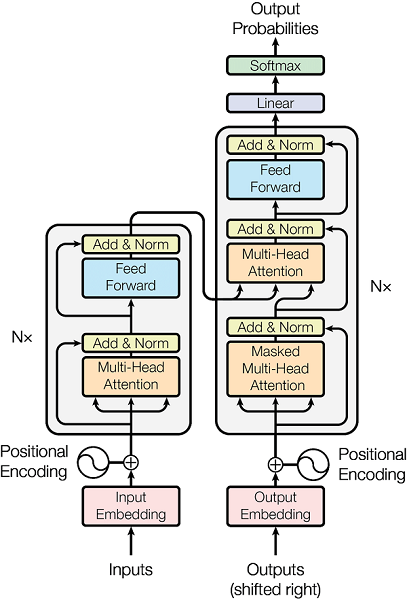
\includegraphics[width=9cm]{img/transformer.png}

  \caption{The overall schema of the Transformer model. Inputs are summed with
    positional encodings. Encoder processes the input in $N$ stack layers. Each
    encoder layer consists of self-attention and feed-forward sub-layer. Layers
    are interconnected with residual connections and layer normalization is
    applied on the output of each layer. The decoder stack uses three
    sub-layers, where the additional cross-attention layer attends to the
    encoder output. We show the original image from
    \citet{vaswani2017attention}.}
  \label{fig:transformer}
\end{figure}

% - - - - - - - - - - - - - - - - - - - - - - - - - - - - - - - - - - - - - - -
\paragraph{Positional Encoding.} Since the self attention is a commutative
operation, the ordering of the input tokens needs to be modeled explicitly.
The standard technique is to use sinusoidal encodings, proposed in the original
paper. Positional encoding is a vector of the same dimension as the word
embedding which is computed using the position of the word on the input.
The $2i$-th and $(2i+1)$-th elements of the positional encoding of word on
position $j$ is computed as follows:
%
\begin{equation}
  \begin{split}
    E_{\text{pos}}(j, 2i) &= \sin(j / 10000^{2i/d}) \\
    E_{\text{pos}}(j, 2i + 1) &= \cos(j / 10000^{2i/d})
  \end{split}
\end{equation}
%
where $d$ is the \emph{model dimension}. This number is equal to the dimension
of the word embeddings. Before an input word $w_i$ is processed by the network,
the positional encodings are added to the word embeddings:
\begin{equation}
  E(w_i) = E(w) + E_{\text{pos}}(i)
\end{equation}

% - - - - - - - - - - - - - - - - - - - - - - - - - - - - - - - - - - - - - - -
\paragraph{Self-Attention.} The key component of the Transformer model is the
self-attention. As the name suggests, self-attention is run with the same set
of states used as both queries, keys, and values. Scaled dot-product is used as
the similarity metric, so the attention itself does not use any trainable
parameters. Formally, self-attention is defined as function:
%
\begin{equation}
  \mathcal{A}(Q,K,V) = \softmax \left( \frac{QK^\top}{\sqrt{d}} V  \right)
  \label{eq:scaled-dot-product}
\end{equation}
%
where the values $Q, K, V \in \mathbb{R}^{T \times d}$ ($T$ being the sequence
length) are computed from the same input, usually using a linear projection.

Self-attention sub-layers are used both in the encoder and the decoder. Because
the decoder is autoregressive, the self-attention module needs to be
constrained to attend only to the preceding states (so the model does not
``glance into the future''). This is implemented by applying a triangular mask
on the attention query and key matrix, hence the name \emph{masked
  self-attetnion}.

% - - - - - - - - - - - - - - - - - - - - - - - - - - - - - - - - - - - - - - -
\paragraph{Multi-Head Attention.} Instead of running a single self-attention
per layer, the model structure is enriched by splitting the self-attention into
multiple \emph{heads}. First, each state is projected into $h$ triples of
queries, keys, and values. Then, self-attention is computed on each triple.
Finally, the self attention outputs are mixed together into a single output
sequence:
%
\begin{equation}
  \mathcal{A}^h(Q, K, V) = \sum_{i=1}^h C_i W_i^O \\
\end{equation}
%
where $W_i^O \in \mathbb{R}^{d_h \times d}$ is a parameter matrix used for
projecting the outputs from the individual attention heads into a single
output, and
%
\begin{equation}
  C_i = \mathcal{A}(QW_i^Q, KW_i^K, VW_i^V)
\end{equation}
where $W_i^Q, W_i^K, W_i^V \in \mathbb{R}^{d \times d_h}$ are trainable
matrices that project the states to inputs for the $i$-th attention head
(defined in Equation \ref{eq:scaled-dot-product}). In self-attention,
$Q = K = V \in \mathbb{R}^{T \times d}$ is the set of $T$ states of the current
layer.

% - - - - - - - - - - - - - - - - - - - - - - - - - - - - - - - - - - - - - - -
\paragraph{Cross-Attention.} Each layer in Transformer encoder consists of a
self-attention and a feed-forward sub-layer. The decoder inserts an
\emph{encoder-decoder attetnion}, or \emph{cross-attention} layer.  The
cross-attention layer functions exactly like self-attention layer, but the
queries $Q$ are the decoder states (i.e. the output of the preceding
self-attention), and the keys and values $K = V$ correspond to the encoder
output states.

% - - - - - - - - - - - - - - - - - - - - - - - - - - - - - - - - - - - - - - -
\paragraph{Feed-Forward Layer.} Each Transformer layer consists
of self-attention, optionally a cross-attention, followed by a feed-forward
network. This feed-forward network uses the same parameters for all positions
along the state sequence. The network takes a state $x$ and feeds it through a
single hidden layer with a ReLU activation:

\begin{equation}
  \mathcal{F}(x) = \max(0, W_1^Fx + b_1^F)W_2^F + b_2^F
\end{equation}
where $W_1^F \in \mathbb{R}^{d \times d_f}$, $b_1 \in \mathbb{R}^{d_f}$,
$W_2^F \in \mathbb{R}^{d_f \times d}$, and $b_2^F \in \mathbb{R}^d$ are the
weight and bias parameters of the feed-forward network $\mathcal{F}$, and $d_f$
is the dimension of the hidden state.

% - - - - - - - - - - - - - - - - - - - - - - - - - - - - - - - - - - - - - - -
\paragraph{Residual Connections and Layer Normalization.} As a post-processing
step, the output of each sub-layer is connected with the output of the previous
sub-layer with residual connections. \JH{zkontrolovat jestli se to definovalo v
  Deep Architectures, stejně jako Layer Norm.} Similarly to the
\glsentryshort{rnn}-based deep architectures, layer normalization is used in
combination, which ties all states in the sub-layer stack into a shared vector
space.

% - - - - - - - - - - - - - - - - - - - - - - - - - - - - - - - - - - - - - - -
\paragraph{Model Hyperparameters.} The parameters that control the model size
are the model dimension $d$, the number of attention heads $h$, the dimension
of the feed-forward hidden layer $d_f$, and the number of Transformer layers in
the encoder and decoder stack. Note that the dimension of keys and values in a
single attention head $d_h$ is commonly set to be $d / h$, but can be
customized as well.  As a regularization, dropout \citep{srivastava2014dropout}
is applied with rate $P_d$ to the output of each sub-layer before
normalization.

The authors of the architecture propose two presets for these parameters, named
\emph{base} and \emph{big}. Table~\ref{tab:transformer-hyperparams} shows the
hyperparameter values for these two settings.

\begin{table}
  \centering
  \begin{tabular}{lrrrrrr}
    \toprule
      & \# of layers &  $d$  &  $h$  & $d_h$ & $d_f$ & $P_d$ \\
    \midrule
    Transformer base  & 6 &  512  & 8 & 64 &  2,048 & 0.1 \\
    Transformer big  & 6 &  1,024  & 16 & 64 &  4,096 & 0.3 \\
    \bottomrule
  \end{tabular}
  \caption{The hyperparameter values for Transformer base and big variants.}%
  \label{tab:transformer-hyperparams}
\end{table}


% ------------------------------------------------------------------------------
\section{Training}
\label{sec:training}
% ------------------------------------------------------------------------------

Training of \gls{nmt} models is usually done under \emph{supervised}
conditions, using a dataset of parallel sentences. \JH{move the following to
  the experimental section:} The size of the available data varies a lot with
different language pairs. Although there is no formal definition, when there is
less than a million sentence pairs available, the language pair is reffered to
as being \emph{low-resource}. For many languages, even a million sentences is a
very large number compared to what is actually available. The data quality is
also a factor. For example, when the only available data is crawled from the
web, data cleaning can filter out a major part of the corpus. In this thesis,
we focus on language pairs where the data size is not a major issue and we
simulate the low-resource scenario using Romanian-English translation.

Translation models are trained by minimizing the loss function, usually
expressed by cross-entropy between the output distribution and the one-hot
distribution which assigns the probability of one to the correct target word,
and zero probabilities to the other words. Assuming $y_i$ is the correct target
word at position $i$, $p_{\text{ref}}$ is the one-hot distribution, and $p$ is
the distribution predicted by the model, we have:
%
\begin{equation}
  \begin{split}
    H(p_{\text{ref}}, p) &=  - \sum_{w \in \mathcal{V}} p_{\text{ref}}(w) \log p(w) = \\
    &=  - \log p(y_i)
  \end{split}
\end{equation}
%
where $\mathcal{V}$ is the vocabulary. Note that in autoregressive models, the
output distributions $p$ and $p_{\text{ref}}$ are conditioned on the preceding
target words.

Given model parameters $\theta$, the word-level cross-entropy is summed across
the sentence pairs in the data $D$ to obtain the negative log likelihood of the
dataset $J_{\theta}$:
%
\begin{equation}
  \begin{split}
  J_{\theta} &= - \sum_{(x, y) \in D} \sum_{i = 1}^{T_y} \log p(y_i | x, y_{<i}, \theta) \\
  &= - \sum_{(x, y) \in D} \log p(y | x, \theta)
  \end{split} \label{eq:loss}
\end{equation}
%
where $y_{<i}$ denote the target prefix and $T_{y}$ is the length of the target
sentence $y$. The probability of a sentence can be reformulated using the chain
rule.
\JH{rovnice J hvězdička = argmin J over thetas}

% Since the probability distributions are conditioned on the previously decoded
% tokens, the likelihood of the target sentence is reformulated using the chain
% rule:
% %
% \begin{equation}
%   J_{\theta} = - \sum_{(x, y) \in D} \sum_{i = 1}^{T_y} \log p(y_i | x, y_{<i}, \theta)
% \end{equation}
% %
% where $T_y$ is the length of the target sentence.



% - - - - - - - - - - - - - - - - - - - - - - - - - - - - - - - - - - - - - - -
\paragraph{Teacher Forcing.}
Note that in the equations above, the probability distributions are conditioned
on the reference target prefix, rather than the model outputs. This technique
is known as \emph{teacher forcing}, and is essential for the training
convergence. When the model is exposed to its own outputs from the start of the
training, it will very likely fail to converge.

Teacher forcing, however, brings along a problem called \emph{exposure bias} --
the model is never exposed to its own errors, which makes it less robust
against them.

Methods have been proposed to address this issue, including a curriculum
learning approach which gradually replaces teacher forcing with the model
predictions \citep{bengio2015scheduled}. Other methods focus on sequence-level
training or beam search optimization methods, mostly based on reinforcement
learning \citep{williams1992simple, wiseman-rush-2016-sequence,
  ranzato2016sequence}. However, none of these methods was widely adopted, and
current models are believed to be capable of recover from their errors despite
being explicitly trained to do so.

% - - - - - - - - - - - - - - - - - - - - - - - - - - - - - - - - - - - - - - -
%\paragraph{RNNs vs Transformer Training.} A significant difference in training
%\glspl{rnn} and the Transformer model is

% - - - - - - - - - - - - - - - - - - - - - - - - - - - - - - - - - - - - - - -
\subsection{Training Methodology}
\label{sec:training:methodology}
% - - - - - - - - - - - - - - - - - - - - - - - - - - - - - - - - - - - - - - -

In this section, we go through the common techniques for successful training of
\gls{nmt} models. These include data cleaning and augmentation methods,
optimization settings, and hardware considerations.

% - - - - - - - - - - - - - - - - - - - - - - - - - - - - - - - - - - - - - - -
\paragraph{Data Cleaning.} With a few exceptions for high-resource languages,
the training data are usually acquired from the Web. Depending on the data
source and the extraction technique, there is a level of noise present in the
data. In many cases, it is necessary to consider data cleaning before training
any models.

The basic data cleaning techniques are rule-based and include language
identification, and filtering sentence pairs with odd characters or length
ratios. Deduplication may be considered, but might be harmful when it removes
short sentences which appear commonly in the given language. For example, if
English sentences ``Thank you'' and ``Thank you xxx'' both appear in the data
as translations of the Czech ``Děkuji'', they might get equal probabilities
when deduplication is used. Without deduplication, the frequency of the correct
translation would be much higher in the training data.

An advanced data cleaning technique is dual conditional cross-entropy filtering
\citep{junczys-dowmunt-2018-dual}. Using two translation models trained on
clean data in opposite directions, each sentence pair is scored according to
the cross entropies assigned by the translation models to the sentence
pair. When the cross entropies differ, or when both cross entropy scores are
high, the score is low. When the cross entropies are similar and are low, the
score is high. After scoring, low-scoring sentence pairs are removed from the
data using an empirically set threshold.

% - - - - - - - - - - - - - - - - - - - - - - - - - - - - - - - - - - - - - - -
\paragraph{Data Augmentation.} The size of the training data is a key factor to
model performance. In rare cases of high-resource languages, there is enough
parallel data available to train a decent translation model. But even for these
languages, data augmentation methods, namely \emph{backtranslation} are used
to create bigger data and therefore to improve the model performance.

Backtranslation is a simple technique for incorporating target-side monolingual
data in a \gls{nmt} model \citep{sennrich-etal-2016-improving}. For a given
translation direction, we first translate the monolingual data from the target
language to the source language using a previously trained model. Then, we mix
the synthetic source-language data along with the authentic target-language
data into our training corpus. When the parallel-to-monolingual data size ratio
not balanced, one can consider oversampling the smaller part of the corpus to
mitigate this. Recently, \citet{caswell-etal-2019-tagged} showed that labeling
the synthetic data with a special token improves the translation quality. As
pointed out by \citet{marie-etal-2020-tagged}, this helps because the model is
less prone to overfitting to this type of data.

\emph{Knowledge distillation} \citep{kim-rush-2016-sequence} is another data
augmentation technique. Unlike backtranslation, knowledge distillation is used
mainly for improving the model efficiency, both in terms of memory and speed.
Also unlike backtranslation, we use target-language synthetic data. In the
simplest setting, we use a well-trained and large \emph{teacher} model to
translate its own training data. Then, we train a smaller (and therefore faster
and smaller) \emph{student} model on the outputs of the teacher model. This
technique shows that for a small sacrifice of the translation quality, we can
get interesting improvements in terms of speed, which is useful for deploying
the models in a limited environment, such as a mobile device.

% - - - - - - - - - - - - - - - - - - - - - - - - - - - - - - - - - - - - - - -
\paragraph{Batching.} In Equation \ref{eq:loss}, the loss function
$\mathcal{J_\theta}$ is defined as a sum of sequence-level losses over dataset
$D$. We use gradient descent to find parameters $\theta$ which minimize the
loss value. However, the exact computation of the gradient is inefficient
because it requires one pass through the whole dataset. Therefore, we estimate
the gradient on a small sample of the training data, called a \emph{mini
  batch}, or simply a batch. This method is called \emph{stochastic gradient
  descent}.

The size of a mini batch is an important parameter and its value can have a
large impact on the training convergence. Bigger batches provide better
gradient estimates, but require more memory, which is an issue when using a
GPU.

\JH{shuffling goes here}

\JH{optimizer delay perhaps also here}

% - - - - - - - - - - - - - - - - - - - - - - - - - - - - - - - - - - - - - - -
\paragraph{Optimization.}


% - - - - - - - - - - - - - - - - - - - - - - - - - - - - - - - - - - - - - - -
\paragraph{Parameter Initialization.}

\JH{random initialization vs pretraining / transfer learning}


% - - - - - - - - - - - - - - - - - - - - - - - - - - - - - - - - - - - - - - -
\paragraph{Early Stopping.} To avoid overfitting, the model should be regularly
tested on a validation dataset over the course of the training. The validation
data should not overlap with the training or test data. Once the model stops
improving on a chosen validation metric, the training process is
interrupted. This method is reffered to as \emph{early stopping}. Usually, the
validation metric is either the cross-entropy loss, or the target evaluation
metric, such as BLEU. An alternative early stopping method is to save the
parameters of the best performing model on validation.

% - - - - - - - - - - - - - - - - - - - - - - - - - - - - - - - - - - - - - - -
\paragraph{Hardware.}




% ------------------------------------------------------------------------------
\section{Autoregressive Decoding}
\label{sec:training-vs-inference}
% ------------------------------------------------------------------------------

The models we described in the sections above are \emph{autoregressive} -- the
output tokens are predicted left-to-right, while every decision is conditioned
on the previously generated outputs. With this property, there comes an
important distinction in behavior between training and decoding. Whereas during
training, the ground-truth data are used to simulate the previous decisions,
during decoding, the ground truth is unknown and therefore the model needs to
rely solely on its own decisions. This constitutes a theoretical problem,
called \emph{exposure bias} -- the model is never exposed to its own errors
during training.

In the RNN-based models, the difference between training and decoding is
minimal. The model execution is done the same way, with the one exception of
providing ground-truth data during training. Another exception is that the final
softmax does not need to be computed during greedy decoding (there is no need
for normalized distribution if we are interested only in the token with maximum
probability), but is still needed for beam search.

The Transformer models are quite different in this aspect. Since there is no
recurrence operation which requires accumulation of information in a hidden
state, the network can be trained on a whole ground-truth sentence in one step.
The only requirement is to prevent the decoder self-attention from attending to
the future positions. However, during training, the model is still conditioned
on its own decisions. \JH{tohle neni pravda}




\section{Evaluation}
\label{sec:evaluation}

The problem of \gls{mt} evaluation is almost as challenging as \gls{mt} itself.
The most reliable method for assessing the quality of \gls{mt} systems remains
human evaluation.  Since the adoption of statistical approach for \gls{mt}
\citep{brown-etal-1993-mathematics,koehn-etal-2003-statistical}, the demand for
automatic translation quality metrics grew larger, as the models often need to
be validated several times during training.

Perhaps the best-known automatic \gls{mt} metric is BLEU
\citep{papineni2002bleu}.  Despite a long term effort led by the organizers of
the WMT Metrics shared task to create an automatic evaluation metric that would
be better correlated with scores assigned by humans, BLEU continues to be the
most widely used metric in the contemporary literature. However, over the nearly
two decades of using BLEU, it has been criticized for being prone to errors due
to outliers or being too inaccurate when the score itself is low.
\citep{callison-burch-etal-2006-evaluating,bojar-etal-2010-tackling,reiter2018structured,mathur-etal-2020-tangled}

\JH{evaluation of decoding speed -- latency, throughput}



%%% Local Variables:
%%% mode: latex
%%% TeX-master: "thesis"
%%% End:

%\begin{markdown}

# Context #
... this needs some

pohádka:

* majority of nmt systems are sentence-level
* document-level methods exist and are on the rise
* seems like context helps
* worries: bleu as a metric no longer credible
* another research on adding context
    - factored input
	- multimodal translation
	- multi-source translation
	

\end{markdown}

%\include{04-mmt}
% %%%%%%%%%%%%%%%%%%%%%%%%%%%%%%%%%%%%%%%%%%%%%%%%%%%%%%%%%%%%%%%%%%%%%%%%%%%%%
\chapter{Non-Autoregressive NMT}
\label{chap:nat}
% %%%%%%%%%%%%%%%%%%%%%%%%%%%%%%%%%%%%%%%%%%%%%%%%%%%%%%%%%%%%%%%%%%%%%%%%%%%%%

The efficiency of \gls{mt} models is often crucial in real-world applications.
Most commercial \gls{nmt} models are available through a cloud-based service,
such as Microsoft Translator\footnote{\url{https://microsoft.com/translator}}
or Google Translate\footnote{\url{https://translate.google.com}}. Scaling
cloud-based solutions for large user bases is simple but costly. But even with
a large pool of computational resources, it is worthwhile to implement
optimizations which decrease the model latency and improve the user experience.

% lokální modely maj tu výhodu, že to běží u mně, takže to jde pouyžít offline
% a taky se nemusím bát o svoje soukromý data. ale jsou pomalý.

Locally-deployed \gls{nmt} models provide a number of advantages over
cloud-based solutions. First, the service does not rely on internet
connection. Second, the data are not being sent to a 3rd party server, and
therefore it is suitable for translating private or confidential data.
However, without optimization, running state-of-the-art translation models
locally often requires specialized hardware, such as one or more GPU
cards. Otherwise, the time for translating a single sentence can easily reach
more than a second on a standard CPU.

Higher decoding speeds can be achieved by model optimization. In their 2019
submission to the \gls{wngt} shared task on efficiency,
\citet{kim-etal-2019-research} successfully employed knowledge distillation,
quantization, shortlisting \citep{jean2015using} and a simpler recurrent unit
design to bring the throughput of the translation model up to 3,600 words per
second on a CPU, for a modest drop in the BLEU score. Following this
submission, \citet{bogoychev-etal-2020-edinburghs} reported further
improvements with attention head pruning \citep{voita-etal-2019-analyzing}. The
work has been a part of the Bergamot research project, which aims to bring
offline translation models into a browser (\JH{cite}).

% vedle toho tu jsou neautoregresivní modely který se na to snaží jít jinak

\Gls{nar} models present an alternative approach to model optimization, using a
different architecture and decoding algorithm which has lower time complexity.
In \gls{nmt}, a non-autoregressive decoding algorithm does not access the
previously decoded outputs, imposing conditional independence on the output
token probability distributions. This assumption allows parallelization of the
decoding which can significantly reduce the latency of the translation
system. On the other hand, it also presents a challenge to the language model,
which usually leads to poorer translation quality.

The research presented in this thesis is focused on the usefulness of \gls{nar}
models for translation (\glsentryshort{nat}\glsunset{nat}) in the quest for
faster translation models. We first analyze the \gls{nat} models alone and
assess the necessary techniques needed to match the quality of \gls{ar} models.
Then, we adapt the optimizations successfully used in \gls{ar} models for
\gls{nar} models and evaluate the additional speed gains.

This chapter begins with an overview of the non-autoregressive methods (Section
\ref{sec:nat-methods}). In Section \ref{sec:nat-ctc}, we introduce
non-autoregressive \gls{nmt} with \gls{ctc}. \JH{rewrite following commented:}
% We present our experiments with \gls{ctc} in Section
% \ref{sec:ctc-experiments}. We summarize our contributions and outline the
% possible future efforts in Section \ref{sec:nat-future}.


% ------------------------------------------------------------------------------
\section{Related Work}
\label{sec:nat-methods}
% ------------------------------------------------------------------------------

This section presents the key concepts in non-autoregressive \gls{nmt}. We
first describe the principles that most of the related literature has in
common. Then, we provide a survey of notable approaches to \gls{nat}.

% ------------------------------------------------------------------------------
\paragraph{Conditional Independence.} The defining feature of a
non-autoregressive model is the conditional independence of the output
distributions across time steps. Recall Equation \ref{eq:output-distribution}
which defines the output distribution for autoregressive models:
%
\begin{equation}
  p(y|x) = \prod_{t=1}^{T_y}p(y_t|y_{<t},x,\theta).
  \tag{\ref{eq:output-distribution}}
\end{equation}
%
Unlike Equation \ref{eq:output-distribution}, \Ac{nat} models do not condition
the output token probabilities on the previously decoded outputs $y_{<t}$.  The
probability of an output sentence $y$ given an input sequence $x$ can then be
modeled as:
%
\begin{equation}
  p(y|x) = \prod_{t=1}^{T_y}p(y_t|x,\theta).
  \label{eq:nat-output-distribution}
\end{equation}

Although technically possible, making the outputs in \acs{rnn}-based models
conditionally independent does not reduce the decoding time because in
\acsp{rnn}, each state depends on the value of the preceding state. However, in
the Transformer model, the hidden states in one layer depend only on the states
from the previous layer. This allows for parallelization on the layer level.

Since the outputs are conditionally independent, the Transformer decoder cannot
work with the previously decoded outputs. In the following paragraphs, we
discuss the necessary alterations to the Transformer architecture.  First, the
decoder needs to know the sentence length. Second, we need to supply the
decoder inputs. Third, the causal mask in the decoder self-attention is now
unnecessary.

% ------------------------------------------------------------------------------
\paragraph{Target Length Estimation.} In a standard NMT model such as the
Transformer or an \glsxtrshort{rnn}-based model with attention, the length of
the output sentence is modeled implicitly by using the special end-of-sentence
(\eos{}) token. Equations \ref{eq:output-distribution} and
\ref{eq:nat-output-distribution} work with the sentence length implicitly,
assuming that the last token $y_{T_y}$ is the \eos{} token and that \eos{} does not
appear among the previous tokens $y_{<T_y}$.

The probability distribution in Equation \ref{eq:nat-output-distribution} can
be factorized to express the estimation of the target sentence length
explicitly, leaving out the \eos{} symbol from the mathematical model:
\begin{equation}
  p(y|x) = p_L(T_y|x, \theta) \cdot \prod_{t=1}^{T_y}p(y_t|x,\theta).
  \label{eq:explicit-length}
\end{equation}


% When using Equation \ref{eq:output-distribution} to model probability
% distribution over the set of all possible sentences, the probabilities assigned
% to longer sentences are considerably lower than the probabilities of sentences
% which are short. This follows from the multiplication of probabilities, which
% are numbers between zero and one. \JH{další věc je že je ten search space
%   exponenciálně roste -- This follows from the fact that the search space
%   (i.e. the number of all possible sentences of length $T_y$) grows
%   exponentially with $T_y$.}  \JH{odkazat spis na argmax nez na output
%   distribution.} To diminish the negative influence of this property,
% \citet{wu2016google} introduce length normalization to the beam search algorithm
% (\JH{odkazat na eq. v intro do MT}). The normalization acts as a prior imposed
% on the target sentence length distribution.

% It is, however, possible to estimate the target length explicitly.
% \JH{...}

\JH{mention these:}
\citep{ghazvininejad2019mask} \citep{mansimov2019generalized}

% ------------------------------------------------------------------------------
\paragraph{Multimodality Problem.} In one of the first attempts to apply a
non-autoregressive model to \gls{nmt}, \citet{gu2017nonautoregressive} describe
the \emph{multimodality problem} which arise when the outputs are conditionally
independent.

When estimating the probability of a word on a given position, there may be
multiple words which get a high probability. These words are the so called
\emph{modes} of the distribution. In autoregressive models, once a word gets
selected, other modes are ignored in the following time steps. However, a
non-autoregressive model does not base the decisions on the preceding ones, so
when multiple positions have multiple modes, the model has no way of knowing
which modes have been selected on other positions.

% This issue is illustrated in Figure \ref{fig:multimodality-problem}.
% \begin{figure}
%   \centering
%   \begin{minipage}{\textwidth}
%     source: thank you

%     \begin{center}
%     \begin{tabular}{cccc}
%       \toprule
%       $y_1$ & $p(y_1|x)$ & $y_2$ & $p(y_2|x)$ \\
%       \midrule
%       vielen & 0.4 & dank & 0.4 \\
%       danke  & 0.3 & schön & 0.3 \\
%       \vdots & & \vdots & & \\
%       \bottomrule
%     \end{tabular}
%     \end{center}

%   \end{minipage}
%   \caption{Illustration of the multimodality problem.}
%   \label{fig:multimodality-problem}
% \end{figure}

A well-known example of the multimodality problem is the translation of the
sentence ``thank you'' into German, which has two equally likely translations:
``vielen dank'' and ``danke schön.'' In this case, the pair of German tokens
``danke'' and ``vielen'' create the two modes on the first position, and the
tokens ``dank'' and ``schön'' are modes on the second position. If an
autoregressive model chooses to generate ``danke'' on the first position, the
token ``dank'' on the second position will no longer be likely. However, when a
non-autoregressive model assigns high probabilities to the correct
translations, it also has to assign high probabilities to the other (incorrect)
two combinations, ``danke dank'' and ``vielen schön''.

% ------------------------------------------------------------------------------
\paragraph{\Ac{nat} with Fertility Model.} Non-autoregressive Transformer
decoder does not receive the previously decoded tokens on the input. A solution
proposed by \citet{gu2017nonautoregressive} is to use a simple fertility model,
which also serves as the explicit target length estimator.

Compared to the autoregressive Transformer model, the model has the following
modifications. First, the inputs to the decoder are made up of the sequence of
encoder inputs, either uniformly stretched to the predicted target sentence
length, or copied using a fertility model. Second, the decoder self-attention
does not use the causal mask since all states can now attend to all other states
in both directions. Third, \emph{positional attention} is added to every decoder
layer where the positional encoding is used as queries and keys, and the decoder
states as values.

In \citet{gu2017nonautoregressive}, the multimodal problem is addressed by
introducing a latent fertility variables $f_1, \ldots, f_{T_x}$ sampled from a
prior distribution. Each $f_i \in \mathbb{N}_0$ denotes the number of times to
copy $x_i$ to the decoder input. The output probability is then conditioned on
the value of the latent variable.
% \begin{equation}
%   p(y|x) = p_L(T_y|x, \theta) \cdot \prod_{t=1}^{T_y}p(y_t|x, z, \theta).
% \end{equation}

The training is done by combining two loss functions -- translation loss and
fertility loss:
\begin{align}
  \mathcal{L}(\theta)  & = \log p(y|x, \theta) \\
                       & = log \sum_{F \in \mathcal{F}} p(F| x, \theta ) p(y | x, F, \theta) \\
                       & \geq \mathbb{E}_{\bar{F} \sim q}
                         \left(
                         \sum_{t=1}^{T_y} \log p(y_t | x, \bar{F}, \theta)
                         + \sum_{t=1}^{T_x} \log p(f_t | x, \theta)
                         \right)
                         + \mathcal{H}(q)
\end{align}
%
where \JH{... describe the equation, or comment it out. Also, what is $\mathcal{H}$?}
%
The fertility model depends on an external module and is not trained end to
end. The authors fine-tune the trained model using reinforcement learning
\citep{williams1992simple}.

During decoding, the marginalizing over all possible fertility values is intractable. Therefore, the authors experiment with three approximation methods -- argmax and average decoding, and \ac{npd}.

% ------------------------------------------------------------------------------
\paragraph{Knowledge Distillation.} To tackle the multimodality problem from
another angle, \citet{gu2017nonautoregressive} propose to use sequence-level
knowledge distillation to create artificial training data
\citep{kim-rush-2016-sequence}. The main idea is that outputs of a teacher
model will have a simpler structure than natural language, limiting the number
of the distribution modes.

According to an ablation study published by \citet{gu-kong-2021-fully}, using
knowledge distillation is a crucial element in training non-autoregressive
translation models, regardless the actual method used.

% ------------------------------------------------------------------------------
\paragraph{Iterative Refinement.} Another attempt to introduce latent variables
in a non-autoregressive model was proposed by \citet{lee2018deterministic}.
Instead of modelling fertility, the authors introduce $L$ discrete sequential latent
variables interpreted as stages of refinement:
%
\begin{align}
  \begin{split}
    p(y|x) & = \sum_{y^L}
      \left( \prod_{t=1}^{T_y} p(y_t|y^L, x) \right) p(y^L|x) \\
    p(y^L|x) & = \sum_{y^{L-1}}
      \left( \prod_{t=1}^{T_y} p(y_t^L | y^{L-1}, x) \right)
      p(y^{L-1}|x) \\
    \vdots \\
    p(y^0|x) & = \prod_{t=1}^{T_y} p(y_t^0|x)
  \end{split}
\end{align}
%
Each summation in the equations above is computed over the whole space of
possible sequences, and thus, it is intractable for the probablility $p(y|x)$
to be caluculated exactly. To overcome this problem, the authors approximate
the sums with only the element corresponding to the sequence with the largest
probability, $\hat{y}_t = \argmax_{y_t}p(y_t|x)$.\footnote{Note that in
  non-autoregressive model where the probability does not depend on previously
  decoded outputs $y_{<t}$, getting the most probable tokens will also yield
  the most probable sequence.}  Putting it together with the equations above
and moving to the logarithmic domain, we get:
\begin{align}
  \begin{split}
    \log p(y|x) \geq
    & \sum_{t=1}^{T_y} \log p(y_t| \hat{y}^L, x) + \\
    & + \sum_{t=1}^{T_y} \log p(\hat{y}_t^{L}| \hat{y}^{L-1}, x) + \ldots \\
    & + \sum_{t=1}^{T_y} \log p(\hat{y}_t^0 | x). \label{eq:refinement-lowerbound}
    % = & \sum_{l=0}^{L} \sum_{t=1}^{T_Y} \log p(\hat{y}_t^{l+1} | \hat{Y}^l, X)
  \end{split}
\end{align}
%where $Y^0 = X$ and $\hat{y}_t^{L+1} = y_t$.

The initial sequence $\hat{y}_t^0$ is set to $x_{t'}$ where
$t' = (T_x / T_y) \cdot t$, i.e. the source sentence is either squished or
stretched by copying or omitting some of the source words in order to fit the
target sentence length. During training, the length of the reference sentence
is known. During decoding, the authors use a separate model $p(T_y|x)$ for
target length prediction. All probability distributions in the above equations
are modeled with neural networks with shared parameters. In this way, the
number of intermediate refinement steps remains flexible during the decoding.

The latent variable model is trained by minimizing the log-likelihood of the
eference sentence $y^*$ in each of the refinement steps:
\begin{equation}
  \mathcal{L}_{\text{LVM}}(\theta) = - \sum_{l=1}^{L+1} \left(
    \sum_{t=1}^{T_{y^*}} \log p(y_t^* | \hat{y}^{l-1}, x, \theta)
  \right) \label{eq:refinement-lvm-loss}
\end{equation}

In their iterative approach, \citet{lee-etal-2018-deterministic} also discuss
the training of the refinement process from a denoising perspective. Formally,
they introduce an additional denoising autoencoder loss to the model:
%
\begin{equation}
  \mathcal{L}_{\text{DAE}}(\theta) = - \sum_{t=1}^{T_y} \log p(y_t^* | \bar{y}, x, \theta)
\end{equation}
where $\bar{y}$ is a corrupted version of the reference translation $y^*$. The
corruption process is performed on each token with a probability $\beta$. Each
corrupted token is either replaced with a random word from the vocabulary,
copied to its neighbor, or swapped with the neighbor.

During training, the two loss functions are stochastically mixed using a
hyper-parameter $\alpha$, sampled from a Bernoulli distribution.


% ------------------------------------------------------------------------------
\paragraph{Aligned Cross Entropy for \gls{nat}} One problem with using
cross-entropy objective for training \gls{nat} models is that it heavily
penalizes misaligned target words. If a correct word is generated at an
incorrect position in the target sentence, the loss is the same as if the model
generates a completely unrelated word. In autoregressive models, this problem
is avoided with teacher forcing -- the model is provided with the preceding
words from the reference sentence. Without teacher forcing, the alignment
between the predicted distributions and the positions in the reference sentence
is too rigid. One way to address this problem is to consider the alignment as a
latent variable. \JH{add example of misaligned sentence.}

Aligned cross entropy (AXE; \citealp{ghazvininejad2020aligned}) is an objective
function that takes this problem into account. It uses a dynamic programming
algorithm to find the alignment with the minimum cross-entropy loss. \JH{add an
  example of the best alignment}

\JH{skip prediction, skip target in the algorithm}

Formally, ... \JH{doplnit}

In our experiments, we use the \ac{ctc} loss, which is similar to this
approach. Instead of considering the alignment that yields the minimum
cross-entropy loss, the \ac{ctc} algorithm computes the sum of all the possible
alignments. Unlike \ac{axe}, we only consider skipping the predictions, while
not allowing to skip the target positions. We present the \ac{ctc}-based method
in detail in Chapter \ref{chap:nar-nmt-ctc}.



% ------------------------------------------------------------------------------

\paragraph{Blockwise Parallel Decoding for Deep Autoregressive Models.}
\citet{stern2018blockwise} propose a semi-autoregressive approach where chunks
of the target sentence are generated in parallel.

They start with a greedy decoding from an autoregressive model, $p_1$, and
introduce additional ``look-ahead'' models $p_2, \ldots p_k$. In time step $t$,
each model $p_i$ predicts the $(t + i)$-th word in the target sequence given the
same prefix of $t$ previously decoded words.

The decoding process has three stages. First, the block of predictions using the
models $p_1, \ldots, p_k$ is computed. Second, model $p_1$ is used to verify the
$(k-1)$ candidates (which is done in parallel in the Transformer model) and
finds the largest $\hat{k}$ such that decoded words from models $p_i$,
$1 \leq i \leq \hat{k}$ are all considered best by $p_1$. Third, the accepted
$\hat{k}$ words are generated and the decoding process jumps to time step
$t + \hat{k}$.






% ------------------------------------------------------------------------------

\JH{add semiautroegressive paper from emnlp 2018}

\begin{itemize}
%\item iNat \citep{lee2018deterministic} -- iterative refinement
%\item Blockwise \citep{stern2018blockwise}
\item InsT \citep{stern2019insertion} -- insertion transformer
\item CMLM \citep{ghazvininejad2019mask} -- conditional masked language models
\item LevT \citep{gu2019levenshtein} -- Levenshtein transformer
\item KERMIT \citep{chan2019kermit} -- Kermit (arxiv)
\item LaNMT \citep{shu2020latent} -- latent-variable NAR NMT with deterministic inference using a delta posterior
\item SMART \citep{ghazvininejad2020semiautoregressive} -- semi-autoregressive training improves mask-predict decoding
\item DisCO \citep{kasai2020nonautoregressive} -- NAR NMT with disentangled context transformer
\item Imputer \citep{saharia2020nonautoregressive} -- NAR NMT with latent alignments
\end{itemize}

Fully NAT:


% ------------------------------------------------------------------------------

\paragraph{Latent Transformer \citep{kaiser2018fast}.} Latent transformer (fast
decoding in seq. models using discrete latent vars) Use latent variables to make
decoding parallelizable. Auto-encode targets to latent variables which are
predicted autoregressively, then decode from these latent variables in
parallel. Mostly use one eigth of the original sentence length.

Unlike perhaps more common autoencoders, this autoencoder uses discrete latent
variables.  The discretization is studied and decomposed vector quantization
(DVQ) or latent semantic hashing is proposed as best-performing. Generally,
$enc(y) \in \mathbb{R}^D$, where $D$ is latent space dimension. $[K]$ is the
discrete latent space alphabet. $enc(y)$ is discretized to two latent variables
$z_d(y) \in K$ as the latent representation and $z_q(y)$ as input to the
decoder. $\tau_m(i)$ is binary representation of $i$ using $m$ bits.

\textbf{Gumbel softmax} -- produce logits $l = W \text{enc}(y)$,
$W \in \mathbb{R}^{K \times D}$, then take argmax to get $z_d(y)$. Decoder input
$z_q(y)$ is embedding of $z_d(y)$. To make this argmax differentiable, during
training, Gumbel-Softmax trick is used: $g_1, \ldots, g_K$ are sampled from
Gumbel distribution, $g_i \sim -\log(-\log u)$, where $u \sim U(0,1)$, and:
\begin{equation}
  w_i= \frac{\exp((l_i + g_i) / \tau) }{\sum_i exp((l_i + g_i)/\tau)}
\end{equation}
to get $w \in \mathbb{R}^K$, and use $z_q(y) = w \times E$. Gumbel-softmax is
simply used as differentiable sampling from intermediate logits.

\textbf{Improved semantic hashing} -- use rounding bottleneck after squashing
encoder state $z_e(y)$ using saturating sigmoid:
\begin{equation}
  \sigma'(x) = \max(0, \min(1, 1.2 \sigma(x) - 0.1))
\end{equation}
During training, gaussian noise is added before the saturating sigmoid to
encoder states $z_e(y)$: $f_e(y) = \sigma'(z_e(y) + \eta ~ N(0,1)^D)$. Discrete
latent representation, binary vector $g_e(y)$ is constructed by rounding
$f_e(y)$ to zeros and ones. $z_d(y)$ is computed as $\tau^{-1}_{log_K}(g(y))$
(that is, by conversion of $g_e(y)$ from binary to decimal with base $K$). The
input $z_q(y) = e^1_{h_e(y)} + e^2_{1-h_e(y)}$ where $h_e(y)$ is either $f_e$ or
$g_e$ during training, but only $g_e$ during inference.

\textbf{Vector quantizated variational autoencoder (VQ-VAE)} --
$enc(y)\in\mathbb{R}$ mapped on embeddeding $e\in\mathbb{R}^{K\times D}$ as
nearest-neighbor lookup. $z_q(y) = e_k$, whereoq
$k = argmin_{j\in[K]} || enc(y) - e_j ||_2$, latent $z_d(y)$ being $k$. This is
trained with reconstruction loss, and $enc(y)$ being drawn to fixed values of
$z_q(y)$. They also keep moving averages of the embeddings and the counts,
EM-like.

\textbf{DVQ} -- the former has an issue with a few indices receiving the most signal
during training. Proposed two solutions: sliced VQ and projected VQ. In sliced,
idea is to slice $enc(y)$ to smaller vectors and do the nearest neighbor using
the sslices, reconstructing $z_q(y)$ from the results. In projected, instead of
slicing, the vector is projected multiple times to subspace.

The model has three components: autoencoder $ae(y, x)$ which maps $y$ to shorter
latent sequence $l$, latent prediction model $lp(x)$ which produces $l$ out of
$x$, and decoder $ad(l, x)$ which non-autoregressively produces $y$ out of $l$
and $x$. They use two losses with equal weights: recunstruction loss computed
from $ad(ae(y,x),x)$ and latent prediction loss comparing $ae(y,x)$ and $lp(x)$.
The latent predictor is a transformer, the autoencoder is stack of convolutions
with residual connections, and the decoder consists of up-convolutions.

Results measured on WMT'14 EN-DE. Baseline 27.3 BLEU, they achieve 22.5 with
rescoring. p-DVQ and s-DVQ as well as improved semhash are comparable, semhash
seems faster. Latency in the order of 100 ms, 7-8 ms per sentence with batch
size of 64.



% ------------------------------------------------------------------------------
\paragraph{\Gls{nat} with auxiliary regularization}
\citet{wang2019nonautoregressive} use regularization terms to penalize
similarity of hidden states corresponding to dissimilar words(which battles
repeated translations), and to express a reconstruction loss using an external
translation model (in order to battle incomplete translation problem).

% ------------------------------------------------------------------------------
\paragraph{\citep{shao2020minimizing}}



% ------------------------------------------------------------------------------

% ------------------------------------------------------------------------------


% ------------------------------------------------------------------------------

\begin{itemize}
\item vanilla \citep{gu2017nonautoregressive}
\item CTC (to jsme my)
\item NAT-REG \citep{wang2019nonautoregressive} -- NAR NMT with auxiliary regularization
\item bag-of-ngrams \citep{shao2020minimizing} -- Minimizing the bag-of-ngrams diff for NAR NMT
\item Hint-NAT \citep{li2019hint} -- hint-based training for NAR MT
\item DCRF \citep{sun2019fast} -- fast structured decoding for sequence models
\item Flowseq \citep{ma2019flowseq} -- NAR conditional sequence generator with generative flow
\item ReorderNAT \citep{ran2019guiding} -- guiding NAR NMT decoding with reordering information
\item AXE \citep{ghazvininejad2020aligned} -- aligned xent for NAR MT
\item EM+ODD \citep{sun2020em} -- an em approach to NAR conditional seq generation
\item GLAT \citep{qian2020glancing} -- glancing transformer for NAR NMT
\item Imputer \citep{saharia2020nonautoregressive} -- imputer (again)
\end{itemize}

\section{Non-Autoregressive NMT with Connectionist Temporal Classification}
\label{sec:nat-ctc}

\paperdisclaim{This section is based on paper ``End-to-End Non-Autoregressive
  Neural Machine Translation with Connectionist Temporal Classification'',
  joint work with Jindřich Libovický, published at EMNLP 2018.}

In this section, we describe our approach to \glsxtrlong{nat}.

The idea behind our approach is that we do not explicitly estimate the target
sequence length. Instead, we fix the decoder length on an upper limit of the
target length, given by a hyper-parameter. As the decoder input, we use the
encoder states, split and linearly projected to match the decoder state
dimension and the target length.

As a consequence, we allow the model to generate special ``blank'' tokens in
any given time steps. Since the alignment between the reference tokens and the
corresponding output distribution is unknown, we treat it as a latent variable,
and we use the loss function which marginalizes this latent variable out. In
other words, our loss function is the sum of losses given any possible
alignment. This loss, used mostly in speech recognition domain
\citep{graves2006connectionist}, is known as the \glsxtrfull{ctc}. We describe
this function in more detail in Section \ref{subsec:ctc}.

The \gls{ctc} loss is differentiable with respect to the model parameters,
which means we can back-propagate the gradients returned by the \gls{ctc}
computation. Thus, unlike the originally proposed architectures of
\citet{gu2017nonautoregressive}, our model can be trained end to end.


\subsection{Connectionist Temporal Classification}
\label{subsec:ctc}






\section{Improving Fluency using N-gram Language Models}
\label{sec:nat-lm}

\paperdisclaim{This section is based on paper \emph{``Improving Fluency of
  Non-Autoregressive Neural Machine Translation''}, joint work with Zdeněk
  Kasner and Jindřich Libovický, published online at \texttt{arXiv.org}.}




\section{Non-Autoregressive Model Optimizations}
\label{sec:nat-opt}



%%% Local Variables:
%%% mode: latex
%%% TeX-master: "thesis"
%%% End:

% %%%%%%%%%%%%%%%%%%%%%%%%%%%%%%%%%%%%%%%%%%%%%%%%%%%%%%%%%%%%%%%%%%%%%%%%%%%%%
\chapter{Non-autoregressive NMT with Connectionist Temporal Classification}
\label{chap:nar-nmt-ctc}
% %%%%%%%%%%%%%%%%%%%%%%%%%%%%%%%%%%%%%%%%%%%%%%%%%%%%%%%%%%%%%%%%%%%%%%%%%%%%%

In this chapter, we lay grounds for the \gls{nar} approaches studied in this
thesis. We describe our experiments with an architecture based on the \gls{ctc}
loss \citep{libovicky-helcl-2018-end}. \JH{ok to self-cite when sections will
  be based on this?}

% -----------------------------------------------------------------------------
\section{Connectionist Temporal Classification}
\label{sec:ctc}
% -----------------------------------------------------------------------------

\Gls{ctc} \citep{graves2006connectionist} is a method for training neural
networks on sequential data. Originally applied to the phonetic labelling task,
but later successfully adapted in related areas, including \gls{asr} or
handwriting recognition \citep{liwicki2007novel, eyben2009speech,
  graves2014towards}.

The main strength of \gls{ctc} becomes evident in tasks where the input and
output labels are weakly or not at all aligned, for example in situations where
the observed input sequence is considerably longer than the target output
sequence -- hence the application to \gls{asr}, where the number of extracted
features per second is higher than the number of phonemes uttered per second.
\JH{Confirm this.}

Training neural networks with \gls{ctc} is independent on the actual neural
network architecture. The \gls{ctc} loss function can be applied on any network
with sequential outputs. Thus, this method is applicable to both \glspl{rnn}
and the Transformer model.

Models trained with the \gls{ctc} assume that the alignment between the input
(e.g. a group of frames in an audio signal) and the output (e.g. a phoneme)
states is unknown. A variable number of frames in a row can encode a single
phoneme. Similarly, in translation, multiple words in the source language may
correspond to any number of (even non-consecutive) words in the target
language.

The idea behind \gls{ctc} is to allow some states to produce no output. This is
realized by introducing a special blank token in the target vocabulary.
Optionally, identical outputs produced by multiple consecutive states may be
merged and considered a single output. Because of these properties, there are
groups of equivalent output sequences, which all represent the same target, as
illustrated in Figure~\ref{fig:ctc-equivalent-sequences}.

\begin{figure}
  \centering
  \begin{minipage}{\textwidth}
    \begin{equation*}
        \text{a cat sat on a mat} =
        \begin{cases}
          & \text{a <blank> cat sat on a <blank> mat} \\
          & \text{a a cat cat sat on a mat} \\
          & \text{a <blank> cat cat sat on a mat} \\
        \end{cases}
    \end{equation*}
  \end{minipage}
  \caption{A group of output sequences of equal length which all represent the
    same target in CTC.} %
  \label{fig:ctc-equivalent-sequences}
\end{figure}

In the standard sequence-to-sequence architectures, the value of the loss
function is defined as the sum of the cross entropies of each output state with
respect to the target sequence (see Equation \ref{eq:loss}). In \gls{ctc}, the
loss is defined as the sum of cross-entropy losses of all of the output
sequences equivalent to the given target sequence:
%
\begin{equation}
  J_{\theta}^{\text{CTC}} = - \sum_{(x, y) \in D} \sum_{y' \sim y}  \log p(y' | x, \theta)
  \label{eq:ctc-loss}
\end{equation}
%
where $\sim$ denotes the equivalence relation.  \JH{$J_{\theta}$ should perhaps
  be $J(\theta)$. Also, consider the $\sim$ sign.}

The inner summation in Equation \ref{eq:ctc-loss} is computed over all possible
sequences equivalent to the label sequence. For technical purposes, the label
sequences are limited to a fixed length, which greatly reduces the number of
acceptable hypotheses. However, the number of equivalent hypotheses of a given
length still grows exponentially with the sequence length -- in \gls{ctc}, the
fixed length is always set to be longer than the label sequence. \JH{confirm
  the exponential claim}

The summation over the large set of equivalent sequences can be
implemented using dynamic programming. When both the length of the output and
the length of the target sequences are known, there is a constant number of the
blank tokens to be generated. The process of computing the loss of the whole
output sequence is divided into computing the partial losses with respect to
the possible label prefixes.

\begin{figure}
  \centering

  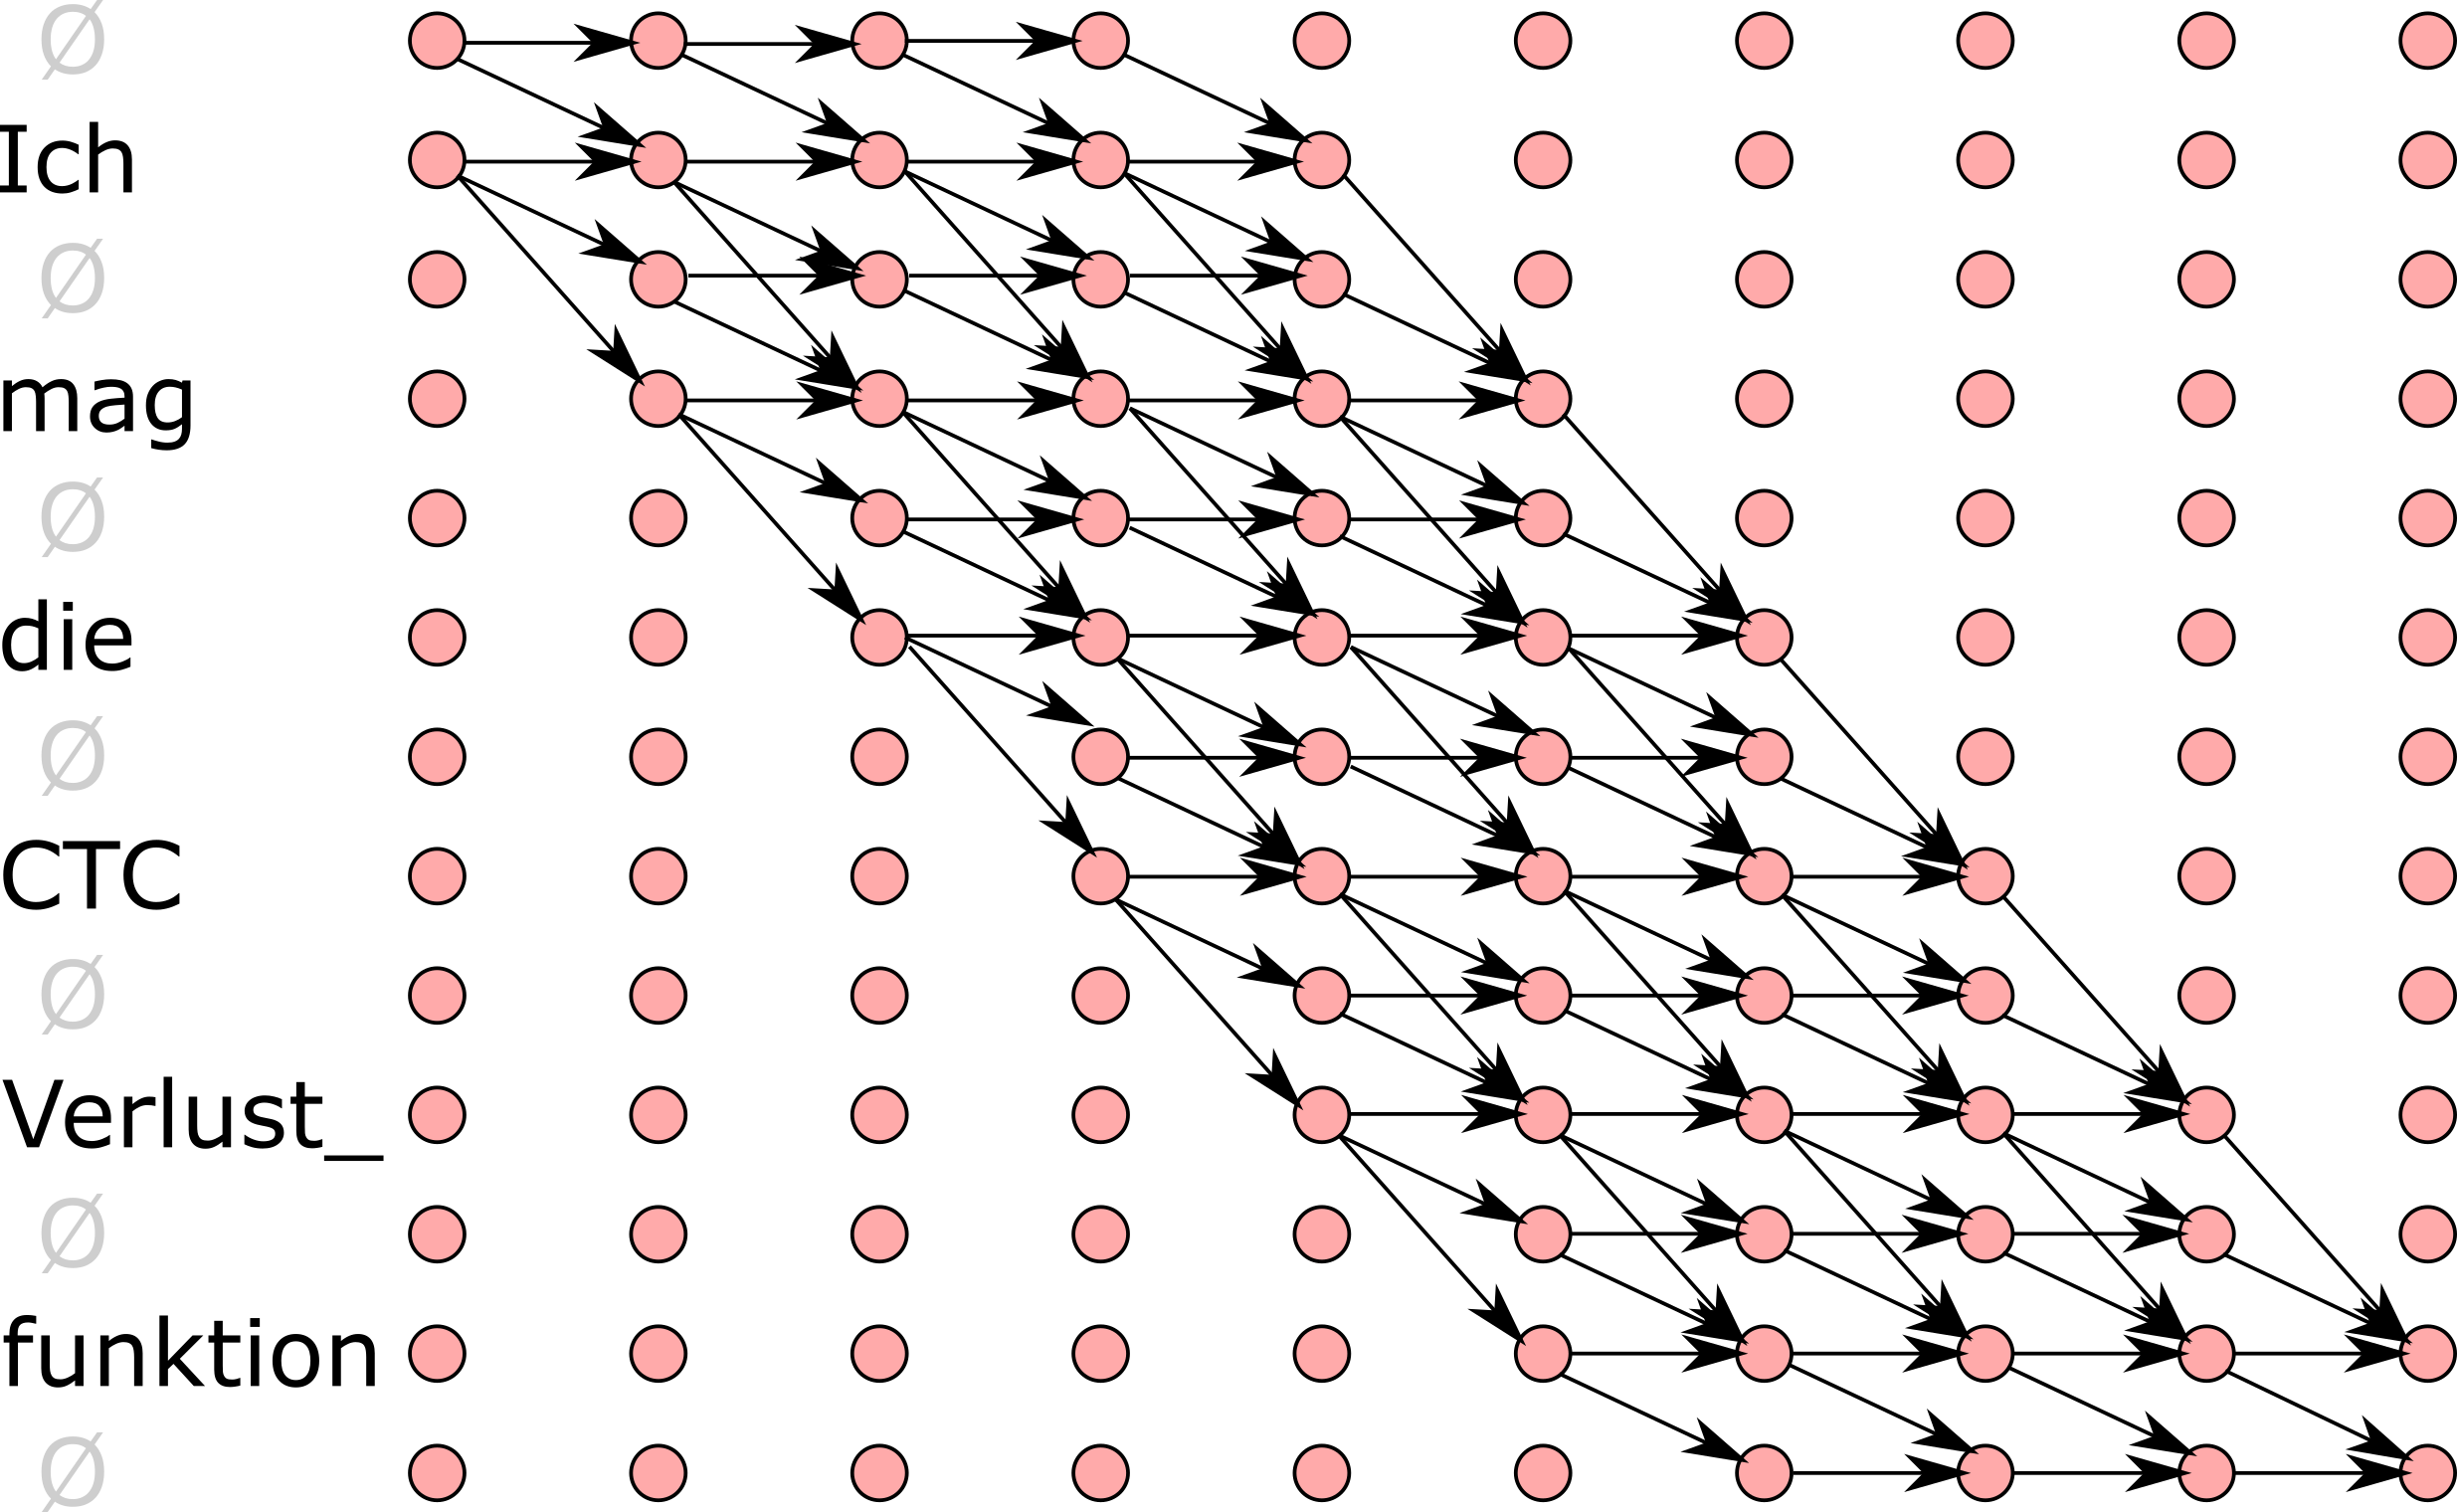
\includegraphics[width=13cm]{img/ctc_schema.png}

  \caption{An illustration of the algorihm for the CTC loss computation. Each
    node denotes producing either a token from the label sequence, or the blank
    token. Each path from one of the two top-left nodes to one of the two
    bottom-right nodes corresponds to one of the equivalent sequences.  }
  \label{fig:ctc-dynamic-programming}
\end{figure}

The \gls{ctc} loss computation is illustrated in Figure
\ref{fig:ctc-dynamic-programming}. The rows represent tokens from the label
sequence plus the optional blank tokens. The columns represent the output state
sequence.  Each node in the graph denotes generating a label from an output
state. The arrows show valid transitions between the generation steps. An arrow
can only go down one or two rows, or horizontally.  The horizontal arrows
denote repeated generation of the same label. These labels are later merged to
form a single output. An arrow can only go two rows down when the skipped row
corresponds to the blank token, so no target tokens are left out. Each path in
the diagram therefore shows one of the equivalent sequences that lead to
generating the given label sequence.

Using the idea that many of the paths from left to right in the diagram share
segments, we can apply dynamic programming to compute the sum of losses across
all paths without the need to enumerate each of them. A node on coordinates
$(i,j)$ stores the accumulated losses for the all path prefixes that lead to
the node, added with the negative log likelihood of the label on the $i$-th row
being generated by the $j$-th output state. The two bottom-right nodes then
store the sum of losses of all the paths.


\JH{doplnit}
The training of the network with \gls{ctc} is done
by minimizing the \gls{ctc} loss function, which is defined as follows.

% -----------------------------------------------------------------------------
\section{Model Architecture}
\label{sec:ctc:arch}
% -----------------------------------------------------------------------------

As said in the previous chapter, training models with \gls{ctc} does not impose
any requirements on the model architecture. In our experiments, we aim for a
reasonable comparison between our proposed approach and the state-of-the-art
autoregressive models. We adapt the Transformer model and use similar
hyper-parameters where applicable.

Non-autoregressive models generate the outputs in parallel, which requires that
the output length is known beforehand. In autoregressive models, the end of
sequence is indicated by a special end symbol, and the constraint on maximum
length is merely a technical aspect.

To leverage the ability to output empty tokens to the full extent, the output
length should be set to a higher number than the length of the target sequence.
Since the length estimation does not need to be accurate, we select a number
$k$ and we set the target sequence length to be $k$ times longer than the
source length. Note that in case the selected length is shorter than the label
sequence, the model will not be able to generate the whole target sequence.


\begin{figure}
  \centering

  \def\inputsize{7}

\begin{tikzpicture}[]

\draw (\inputsize / 2 + 0.1, -0.1) node {Input token embeddings};

\foreach \i in {0,...,\inputsize} {
	\draw (\i,-0.5) rectangle (\i+0.2,-1);
    \draw [->] (\i+0.1,-1) -- (\i+0.1, -1.25);
};

\draw (0, -1.25) rectangle (\inputsize + 0.2, -2.25);
\draw (\inputsize / 2 + 0.1, -1.75) node {Encoder};

\foreach \i in {0,...,\inputsize} {
	\draw [->] (\i+0.1,-2.25) -- (\i+0.1, -2.5);
    \draw[fill=yellow!40] (\i,-2.5) rectangle (\i+0.2,-3);

    \draw [->] (\i+0.1,-3) -- (\i+0.1, -3.25);
	\draw[fill=blue!40] (\i,-3.25) rectangle (\i+0.2,-3.75);
	\draw[fill=red!40] (\i,-3.75) rectangle (\i+0.2,-4.25);

    \draw [dashed,->] (\i+0.1,-4.25) -  - (\i+0.1, -4.75);
    \draw [dashed,->] (\i+0.2,-3.5) .. controls (\i + 0.6, -3.65) .. (\i+0.6, -4.75);

	\draw[fill=red!40] (\i,-4.75) rectangle (\i+0.2,-5.25);
	\draw[fill=blue!40] (\i + 0.5,-4.75) rectangle (\i+0.7,-5.25);

    \draw [->] (\i+0.1,-5.25) - - (\i+0.1, -5.5);
    \draw [->] (\i+0.6,-5.25) - - (\i+0.6, -5.5);
};

\draw (\inputsize + 1.2, -2.75) node {$\mathbf{h}$};
\draw (\inputsize + 1.2, -3.75) node {$W_{\text{spl}}\mathbf{h}$};
\draw (\inputsize + 1.2, -5.00) node {$\mathbf{s}$};

\draw (0, -5.5) rectangle (\inputsize + 0.7, -6.5);
\draw (\inputsize / 2 + 0.5 + 0.1, -6.0) node {Decoder};

\draw [fill=green!80!black!60] (\inputsize / 2 + 0.4,-7.2) circle [x radius=\inputsize / 2 + 0.4, y radius=0.5];
\draw (\inputsize / 2 + 0.6, -7.2) node {Connectionist Temporal Classification};

\foreach \i in {0,...,\inputsize} {
   \draw [->] (\i+0.1,-7.9) - - (\i+0.1, -8.15);
   \draw [->] (\i+0.6,-7.9) - - (\i+0.6, -8.15);
}

\draw  (0+0.1,-8.4) node {$w_1$};
\draw  (0+0.6,-8.4) node {$w_2$};
\draw  (1+0.1,-8.4) node {$w_3$};
\draw  (1+0.6,-8.4) node {$\varnothing$};
\draw  (2+0.1,-8.4) node {$w_4$};
\draw  (2+0.6,-8.4) node {$\varnothing$};
\draw  (3+0.1,-8.4) node {$w_5$};
\draw  (3+0.6,-8.4) node {$w_6$};
\draw  (4+0.1,-8.4) node {$\varnothing$};
\draw  (4+0.6,-8.4) node {$\varnothing$};
\draw  (5+0.1,-8.4) node {$\varnothing$};
\draw  (5+0.6,-8.4) node {$w_7$};
\draw  (6+0.1,-8.4) node {$w_8$};
\draw  (6+0.6,-8.4) node {$\varnothing$};
\draw  (7+0.1,-8.4) node {$w_9$};
\draw  (7+0.6,-8.4) node {$\varnothing$};

\draw (\inputsize / 2 + 0.3, -8.95) node {Output tokens / null symbols};

\end{tikzpicture}

  \caption{The scheme of the non-autoregressive architecture with
    state-splitting and CTC. The image is taken from
    \citet{libovicky-helcl-2018-end}.}%
  \label{fig:state-splitting}
\end{figure}


We implement the source-to-target length expansion by linear projections and
state splitting. This mechanism is illustrated in Figure
\ref{fig:state-splitting}. After a given Transformer layer completes its
computation, we linearly project the states
$h_1, \ldots, h_{T_x} \in \mathbb{R}^d$ into $\mathbb{R}^{kd}$. Then, we split
each of these projections into $k$ parts, which results to a $k$-times longer
sequence of states $s_1, \ldots, s_{k \cdot T_x}$ of the original dimension
$d$:
%
\begin{equation}
  s_{ck+b} = \left( W_{\text{spl}} h_c + b_{\text{spl}} \right)_{bd:(b+1)d}
\end{equation}
%
for $b=0 \ldots k-1$ and $c=1 \ldots T_x$ where
$W_{\text{spl}} \in \mathbb{R}^{d \times kd}$ and
$b_{\text{spl}} \in \mathbb{R}^{kd}$ are the trainable projection parameters.

We experiment with two placement options of the state splitting layer. First,
we try placing the state splitting at the end of the Transformer layer
stack. In this scenario, there are 12 Transformer encoder layers, followed by
the state splitting layer, whose outputs are used in the output
projection. Second, we place the state splitting layer in the middle of the
Transformer layer stack, mimicking the 6-layer encoder-decoder architecture of
the autoregressive Transformer model. In the second variant, cross-attention
can be included in the second half of the layers, which attends to the states
right after state splitting.


\section{Baseline Experiments}

\JH{Section with experiments from the 2018 paper. Should show that it works,
  but it's still far from perfect.}


%%% Local Variables:
%%% mode: latex
%%% TeX-master: "thesis"
%%% End:

% %%%%%%%%%%%%%%%%%%%%%%%%%%%%%%%%%%%%%%%%%%%%%%%%%%%%%%%%%%%%%%%%%%%%%%%%%%%%%
\chapter{Experiments}%
\label{chap:experiments}
% %%%%%%%%%%%%%%%%%%%%%%%%%%%%%%%%%%%%%%%%%%%%%%%%%%%%%%%%%%%%%%%%%%%%%%%%%%%%%


As we discussed in Section \ref{sec:nat:discussion}, the flaws in the
evaluation methodology adopted by current research of \ac{nat} models make it
difficult to identify approaches suitable in production-ready conditions.  In
this chapter, we present further experiments with \ac{nat} models trained with
\ac{ctc}. We focus on fair comparison with other non-autoregressive approaches
as well as state-of-the-art optimized autoregressive methods.  In line with our
previous experiments (see Chapter \ref{chap:nar-nmt-ctc}) and also with the
rest of the related work, we conduct experiments on English-German translation.

As previously stated (see Section \ref{sec:nat:principles}), knowledge
distillation \citep{kim-rush-2016-sequence} is a crucial element that brings
the performance of \ac{nar} methods closer to that of \ac{ar} methods. We use
strong \ac{ar} teachers as both our baseline models, and as the source of the
artificial target side data for training of the distilled models. We describe
our teacher models in detail in Section \ref{sec:exp:teachers}

In Section \ref{sec:exp:students}, we describe the training of the \ac{nar}
student models. We follow the approach described in Chapter
\ref{chap:nar-nmt-ctc}. The key changes to the \acs{ctc}-based models include
training the student models on distilled data and using a faster implementation
of the translation system.

In the analysis of the results presented in Section \ref{sec:exp:results}, we
try to connect the separate worlds of \ac{nat} research and the bids to improve
the efficiency of translation models. Our student models outperform all of the
\ac{nar} models in terms of BLEU on the standard \acs{wmt}~14 translation
benchmark. However, at the same time the models score relatively poorly in
comparison to the current state-of-the-art \ac{ar} translation models, which
suggests that the gap in translation quality between \ac{ar} and \ac{nar}
models is still a problem, contrary to some of the claims in the literature
\citep{gu-kong-2021-fully,saharia-etal-2020-non}. We also present an extensive
analysis of the decoding speed under different conditions and conclude that
without future advancements in this field, optimized \ac{ar} models will
continue to achieve superior results over \ac{nar} models.


% ------------------------------------------------------------------------------
\section{Autoregressive Teacher Models}%
\label{sec:exp:teachers}
% ------------------------------------------------------------------------------

\paperdisclaim{This section is based on ``The University of Edinburgh's
  English-German and English-Hausa Submissions to the WMT21 News Translation
  Task'', joint work with Pinzen Chen, Ulrich Germann, Laurie Burchell, Nikolay
  Bogoychev, Antonio Valerio Miceli Barone, Jonas Waldendorf, Alexandra Birch,
  and Kenneth Heafield, published at WMT 2021.}

\noindent
In this section, we describe the experimental settings for training the
autoregressive teacher models, which we used for knowledge distillation of data
for training our non-autoregressive student models.

In our English-German experiments, we use autoregressive models from our
submission to the \ac{wmt} 2021 News Translation Shared Task
\citep{chen-etal-2021-university}. We use these models both as a strong
autoregressive baseline, and as teacher models for generating distilled data
for the non-autoregressive student models, described in the next section.  The
models were trained on cleaned parallel data augmented with backtranslated
monolingual data.

% ------------------------------------------------------------------------------
\paragraph{Data Cleaning.} We prepare the training dataset consisting of the
following parts. First, we used clean parallel data from the Europarl corpus
\citep{koehn-2005-europarl}, the Tilde MODEL -- RAPID corpus
\citep{rozis-skadins-2017-tilde}, and News Commentary corpus from OPUS
\citep{tiedemann-2012-parallel}. Next, we included sources of crawled parallel
data from the web, which are considered noisy. These include Paracrawl
\citep{espla-etal-2019-paracrawl}, Common
Crawl\footnote{\url{https://commoncrawl.org/}}, and WikiMatrix
\citep{schwenk2019wikimatrix}, and the Wikipedia Parallel Titles
Corpus\footnote{\url{https://linguatools.org/tools/corpora/wikipedia-parallel-titles-corpora/}}. Finally,
we used backtranslation \citep{sennrich-etal-2016-improving} of monolingual
data obtained from News Crawl. We trained our own models for generating the
backtranslations, trained on cleaned parallel data, as described below.

On the gathered data (both clean and noisy), we applied filtering techniques to
improve the overall quality of the parallel data. First, we applied a
deterministic rule-based filtering%
\footnote{\url{https://github.com/browsermt/students/blob/master/train-student/clean/}}
and deduplication. We removed all sentence pairs containing non-printing
characters, empty sentences, and sentences longer than 120 words; we also
removed all sentence pairs with length ratio of less than 0.6 (0.4 for
Wikititles), sentences in which over 40\% of characters did not constitute
tokens, and sentences in which more than 50\% was non-alphabetic characters. We
ran language identification using fastText
\citep{joulin-etal-2017-bag,joulin2016fasttext} and removed all sentence pairs
classified as not English-German.

The data sizes before and after the rule-based filtering are shown in Table
\ref{tab:ende-data-sizes}. Note that the vast majority of the training corpus
consists of data from noisy sources.

\begin{table}
  \centering
  \begin{tabular}{lrrr}
    \toprule
    Data source & \multicolumn{2}{c}{Raw size} & \mc{Size after cleaning} \\
    \midrule
    Europarl & 1.83 & \multirow{3}{*}{3.86} & \multirow{3}{*}{3.1} \\
    RAPID & 1.63 & &\\
    News Commentary & 0.40 & & \\
    \midrule
    Paracrawl & 82.64 &  \multirow{4}{*}{91.98} & \multirow{4}{*}{84.6} \\
    WikiMatrix & 5.47 & & \\
    Common Crawl & 2.40 & & \\
    Wikititles & 1.47 & & \\
    \midrule
    \multicolumn{1}{r}{total} & & 95.84 & 87.7 \\
    \bottomrule
  \end{tabular}

  \caption{The sizes of the individual raw corpora before and after rule-based
    cleaning, in millions of sentence pairs.}%
  \label{tab:ende-data-sizes}
\end{table}

To further clean the data, we applied dual cross-entropy filtering, as proposed
by \citet{junczys-dowmunt-2018-dual} and described in the data cleaning
paragraph in Section \ref{sec:training:methodology}.  We trained two
Transformer base models for dual cross-entropy filtering using the clean part
of the data after the rule-based cleaning step.  \JH{Add more details on these
  models, perhaps include the hyperparameters somewhere in an appendix, plus
  add the dev scores}

We score the crawled part of the parallel data using the trained models, and we
sort the sentence pairs according to the score. To estimate how many of the
sentence pairs in the crawled we can consider clean, we train translation
models in both directions on different amounts of the scored data. We used
25\%, 50\%, 75\%, and 100\% of the crawled data, taking the highest-scoring
sentence pairs for training. Based on the score on the development data (the
\ac{wmt} 2019 test set, \citealp{barrault-etal-2019-findings}), we select the
75\% highest-scoring sentence pairs from the crawled data. \JH{rephrase this a
  bit + add details about the models} The develoment scores achieved by the
trained models are shown in Table \ref{tab:dual-cross-entropy-selection}.
% \JH{Add the data sizes after this cleaning step.}

\begin{table}
  \centering
  \begin{tabular}{lrrrr}
    \toprule
    Percentage & 25\% & 50\% & 75\% & 100\% \\
    No. of sentences (M) & 21.9  & 43.9 & 66.5 & 87.7 \\
    \midrule
    En $\rightarrow$ De &  & 43.68 & 43.40 & 42.70 \\
    De $\rightarrow$ En & 41.47 & 41.64 & 42.15 & 42.02 \\
    \bottomrule
  \end{tabular}
  \caption{Development \acs{bleu} scores of the Transformer models trained on
    different amounts of scored crawled parallel data in both directions.}%
  \label{tab:dual-cross-entropy-selection}
\end{table}

% \JH{The following is not true / old:}
% We train our autoregressive models on a mix of the clean data and the
% backtranslations. We use tagged-backtranslation and we oversample the clean
% dataset to form roughly 25\% of the mix. We select the top 100 million sentence
% pairs from the backtranslated data according to Moore-Lewis language modeling
% score. \JH{tento odstavec rozvest aspon na stranku a kus}. We also try using
% the top 150 million. \JH{napsat jinak:} As the size of the clean data is 3.6
% million sentence pairs, we oversample the dataset by a factor of 10 for the 100M
% backtranslation version or 14 for the 150M backtranslation version.

% ------------------------------------------------------------------------------
\paragraph{Backtranslation.} We train four translation models on the filtered
parallel dataset for creating backtranslations
\citep{sennrich-etal-2016-improving}. We use identical Transformer big
hyperparameter settings but we use different random seeds for parameter
initialization. We use the same hyperparameter settings as for the teacher
models. The parameter values are shown in Table \ref{tab:trafo-big-hparams}
% The Transformer big models have a 6-layer encoder and a 6-layer decoder, with
% 16 attention heads in the self-attention and cross-attention, with the model
% dimension of 1,024, and the feed-forward hidden layer dimension of 4,096. We
% use a shared SentencePiece vocabulary of 32,000 tokens.  \JH{Make a table out
% of this.}
We ensemble the four models to translate the monolingual data. \JH{Say more
  about decoding -- beam search, normalization, etc.} \JH{Somewhere we need to
  say that we are using Marian to train all the models in this chapter.}

As the source of the monolingual data, we use the News Crawl datasets from
years 2018, 2019, and 2020, as released by the \acs{wmt} organizers
\citep{bojar-etal-2018-findings,barrault-etal-2019-findings,
  barrault-etal-2020-findings}. In total, we gathered 91 million English
sentences for backtranslation into German and 146 million German sentences for
backtranslation in the other direction. Table \ref{tab:mono-data-sizes} shows
the sizes of the monolingual data before and after applying the rule-based
filtering described in the paragraphs above.

\begin{table}
  \centering
  \begin{tabular}{llrr}
    \toprule
    \multicolumn{2}{l}{Data source}  & \mcl{Raw size}  & \mcl{Size after cleaning} \\
    \midrule
    \multirow{3}{*}{English News Crawl} & 2018 & 18.11 & 17.90 \\
                                     & 2019 & 33.60 & 32.80 \\
                                     & 2020 & 41.43 & 40.33 \\
    \multicolumn{1}{r}{total} & & 93.14 & 91.03 \\
    \midrule
    \multirow{3}{*}{German News Crawl} & 2018 & 38.65 & 37.42  \\
                                     & 2019 & 57.62 & 56.33  \\
                                     & 2020 & 53.67 & 52.46 \\
    \multicolumn{1}{r}{total} & & 149.94 & 146.22 \\
    \bottomrule
  \end{tabular}

  \caption{The sizes of the monolingual data (in millions of sentences) used
    for the training, including rule-based data filtering}%
  \label{tab:mono-data-sizes}
\end{table}

We follow the approach of \citet{caswell-etal-2019-tagged} and we tag the
backtranslated sentences with a special token on a first position, as explained
in Section \ref{sec:training:methodology}.

% ------------------------------------------------------------------------------
\paragraph{Teacher Model Training.}  We train the teacher models on shuffled
concatenation of the authentic parallel and tagged backtranslated data. As with
the models for backtranslation, we train four models with different seeds for
random initialization in each direction. We show the hyperparameter values in
Table \ref{tab:trafo-big-hparams}.

After the training on mixed parallel and backtranslated data converged, we
continued the training of the models on parallel data only.
\JH{Early stopping.}

\JH{Add a table with scores of the teacher models.}

\begin{table}
  \centering
  \begin{tabular}{llr}
    \toprule
    Parameter & Marian config variable & \mcl{Value} \\
    \midrule
    No. of encoder layers & \texttt{enc-depth} & 6 \\
    No. of decoder layers & \texttt{dec-depth} & 6 \\
    Model dimension &  \texttt{dim-emb} & 1,024 \\
    Feed-forward state dimension & \texttt{transformer-dim-ffn} & 4,096 \\
    Attention heads & \texttt{transformer-heads} & 16 \\
    % & transformer-postprocess & dan \\
    % & transformer-postprocess-emb & d\\
    Vocabulary size & & 32,000 \\
    \midrule
    Optimizer method & \texttt{optimizer} & adam \\
    $\beta_1$ & \multirow{3}{*}{\texttt{optimizer-params}} & 0.9 \\
    $\beta_2$ & & 0.998 \\
    $\epsilon$ & & 10\textsuperscript{-9} \\
    No. of batches per update & \texttt{optimizer-delay} & 2 \\
    Fit batch to available memory & \texttt{mini-batch-fit} & true \\
    Learning rate & \texttt{learn-rate}  & 10\textsuperscript{-4} \\
    Learning rate warmup & \texttt{lr-warmup} & 8,000 \\
    Learning rate decay & \texttt{lr-decay-inv-sqrt} & 8,000 \\
    Gradient clipping\footnotemark & \texttt{clip-norm} & 0 \\
    \bottomrule
  \end{tabular}

  \caption{The hyperparameters of the teacher models. The same values were
    used for training the models for backtranslation.}%
  \label{tab:trafo-big-hparams}

\end{table}
% ------------------------------------------------------------------------------
\paragraph{Knowledge Distillation.} The teacher models are used to create
artificial targets for the student models \citep{kim-rush-2016-sequence}. For
each translation direction, we translate the source side of the parallel data
and the authentic monolingual data (in the source language) using ensembled
teacher models. We do not create wholly synthetic datasets by
forward-translating backtranslated data.


% ------------------------------------------------------------------------------
\section{Student Models}%
\label{sec:exp:students}
% ------------------------------------------------------------------------------
\footnotetext{We did not use gradient clipping because of issues in the Marian
  toolkit implementation.  \JH{is there an issue? Also, put this on the right
    page.}}  % JH: Perhaps switch to the footnote package, which can handle
             % that better
% ------------------------------------------------------------------------------

In this section, we describe our non-autoregressive student models. We
implemented the \acs{ctc}-based Transformer architecture in the Marian toolkit
\citep{junczys-dowmunt-etal-2018-marian}. For the computation of the \ac{ctc}
loss, we use the warp-ctc
library,\footnote{\url{https://github.com/baidu-research/warp-ctc/}} an
efficient parallelized implementation for GPUs \citep{amodei-etal-2016-deep}.

We experiment with different hyperparameter settings that control the size of
the student model. Our baseline non-autoregressive model is a big Transformer
model with 6 encoder layers, followed by the state-splitting layer, and another
6 decoder layers. Apart from the \ac{ctc}-specific configuration, we use the
same hyperparameters as in the teacher models, shown in Table
\ref{tab:trafo-big-hparams}. In addition, we train four smaller models based on
the Transformer base hyperparameters -- using model dimension of 512,
feed-forward state dimension of 2,048, and 8 attention heads. Each smaller
model uses a different number of encoder and decoder layers. We show the number
of encoder and decoder layers in Table \ref{tab:student-model-hparams}. In all
settings, we use the splitting factor of 3 in the state splitting layer.

\begin{table}
  \centering

  \begin{tabular}{llrr}
    \toprule
    Model & Base architecture & \mcl{Encoder layers} & \mcl{Decoder layers} \\
    \midrule
    Teacher & Transformer big & 6 & 6 \\
    \midrule
    Large & Transformer big & 6 & 6 \\
    \addlinespace
    Base  & \multirow{4}{*}{Transformer base} & 6 & 6 \\
    Small & & 3 & 3\\
    Micro & & 2 & 2 \\
    Tiny  & & 1 & 1 \\
    \bottomrule
  \end{tabular}

  \caption{The hyperparameters of the student models.}%
  \label{tab:student-model-hparams}
\end{table}

All models were trained for approximately three weeks on four Nvidia Tesla P100
GPUs. Every 8,000 updates of the training, a model checkpoint was saved and
validated. As the validation dataset, we used the concatenation of three
\ac{wmt} test sets, from years 2018, 2019, and 2020
\citep{bojar-etal-2018-findings, barrault-etal-2019-findings,
  barrault-etal-2020-findings}.  Figures \ref{fig:ende-learning-curves} and
\ref{fig:deen-learning-curves} show the training progress of the student
models. Each plot shows the validation \acs{bleu} scores after a given number
of parameter updates.

\begin{figure}
  \centering
  \begin{tikzpicture}[gnuplot]
%% generated with GNUPLOT 5.2p8 (Lua 5.3; terminal rev. Nov 2018, script rev. 108)
%% Thu 14 Oct 2021 01:45:29 PM BST
\path (0.000,0.000) rectangle (13.500,8.000);
\gpcolor{color=gp lt color border}
\gpsetlinetype{gp lt border}
\gpsetdashtype{gp dt solid}
\gpsetlinewidth{1.00}
\draw[gp path] (1.136,1.505)--(1.316,1.505);
\draw[gp path] (12.947,1.505)--(12.767,1.505);
\node[gp node right] at (0.952,1.505) {15};
\draw[gp path] (1.136,2.536)--(1.316,2.536);
\draw[gp path] (12.947,2.536)--(12.767,2.536);
\node[gp node right] at (0.952,2.536) {20};
\draw[gp path] (1.136,3.567)--(1.316,3.567);
\draw[gp path] (12.947,3.567)--(12.767,3.567);
\node[gp node right] at (0.952,3.567) {25};
\draw[gp path] (1.136,4.598)--(1.316,4.598);
\draw[gp path] (12.947,4.598)--(12.767,4.598);
\node[gp node right] at (0.952,4.598) {30};
\draw[gp path] (1.136,5.629)--(1.316,5.629);
\draw[gp path] (12.947,5.629)--(12.767,5.629);
\node[gp node right] at (0.952,5.629) {35};
\draw[gp path] (1.136,6.660)--(1.316,6.660);
\draw[gp path] (12.947,6.660)--(12.767,6.660);
\node[gp node right] at (0.952,6.660) {40};
\draw[gp path] (1.136,7.691)--(1.316,7.691);
\draw[gp path] (12.947,7.691)--(12.767,7.691);
\node[gp node right] at (0.952,7.691) {45};
\draw[gp path] (1.136,1.505)--(1.136,1.685);
\draw[gp path] (1.136,7.691)--(1.136,7.511);
\node[gp node right,rotate=45] at (1.136,1.321) {0 };
\draw[gp path] (2.448,1.505)--(2.448,1.685);
\draw[gp path] (2.448,7.691)--(2.448,7.511);
\node[gp node right,rotate=45] at (2.448,1.321) {100k};
\draw[gp path] (3.761,1.505)--(3.761,1.685);
\draw[gp path] (3.761,7.691)--(3.761,7.511);
\node[gp node right,rotate=45] at (3.761,1.321) {200k};
\draw[gp path] (5.073,1.505)--(5.073,1.685);
\draw[gp path] (5.073,7.691)--(5.073,7.511);
\node[gp node right,rotate=45] at (5.073,1.321) {300k};
\draw[gp path] (6.385,1.505)--(6.385,1.685);
\draw[gp path] (6.385,7.691)--(6.385,7.511);
\node[gp node right,rotate=45] at (6.385,1.321) {400k};
\draw[gp path] (7.698,1.505)--(7.698,1.685);
\draw[gp path] (7.698,7.691)--(7.698,7.511);
\node[gp node right,rotate=45] at (7.698,1.321) {500k};
\draw[gp path] (9.010,1.505)--(9.010,1.685);
\draw[gp path] (9.010,7.691)--(9.010,7.511);
\node[gp node right,rotate=45] at (9.010,1.321) {600k};
\draw[gp path] (10.322,1.505)--(10.322,1.685);
\draw[gp path] (10.322,7.691)--(10.322,7.511);
\node[gp node right,rotate=45] at (10.322,1.321) {700k};
\draw[gp path] (11.635,1.505)--(11.635,1.685);
\draw[gp path] (11.635,7.691)--(11.635,7.511);
\node[gp node right,rotate=45] at (11.635,1.321) {800k};
\draw[gp path] (12.947,1.505)--(12.947,1.685);
\draw[gp path] (12.947,7.691)--(12.947,7.511);
\node[gp node right,rotate=45] at (12.947,1.321) {900k};
\draw[gp path] (1.136,7.691)--(1.136,1.505)--(12.947,1.505)--(12.947,7.691)--cycle;
\node[gp node center,rotate=-270] at (0.016,4.598) {\acs{bleu}};
\node[gp node center] at (7.041,0.215) {Number of updates};
\node[gp node right] at (12.031,3.764) {Large};
\gpcolor{rgb color={0.800,0.000,0.000}}
\gpsetlinewidth{2.50}
\draw[gp path] (12.215,3.764)--(12.579,3.764);
\draw[gp path] (1.241,2.247)--(1.346,4.433)--(1.451,5.134)--(1.556,5.505)--(1.661,5.711)%
  --(1.766,5.856)--(1.871,5.959)--(1.976,6.083)--(2.081,6.145)--(2.186,6.165)--(2.291,6.186)%
  --(2.396,6.330)--(2.501,6.309)--(2.606,6.392)--(2.711,6.371)--(2.816,6.371)--(2.921,6.433)%
  --(3.026,6.474)--(3.131,6.495)--(3.236,6.474)--(3.341,6.495)--(3.446,6.516)--(3.551,6.578)%
  --(3.656,6.578)--(3.761,6.598)--(3.866,6.578)--(3.971,6.578)--(4.076,6.578)--(4.181,6.598)%
  --(4.286,6.619)--(4.391,6.639)--(4.496,6.660)--(4.601,6.701)--(4.706,6.660)--(4.811,6.619)%
  --(4.916,6.681)--(5.021,6.660)--(5.125,6.660)--(5.230,6.681)--(5.335,6.701)--(5.440,6.681)%
  --(5.545,6.722)--(5.650,6.722)--(5.755,6.722)--(5.860,6.742)--(5.965,6.722)--(6.070,6.763)%
  --(6.175,6.763)--(6.280,6.763)--(6.385,6.804)--(6.490,6.763)--(6.595,6.763)--(6.700,6.742)%
  --(6.805,6.804)--(6.910,6.763)--(7.015,6.804)--(7.120,6.784)--(7.225,6.804)--(7.330,6.763)%
  --(7.435,6.804)--(7.540,6.804);
\gpcolor{color=gp lt color border}
\node[gp node right] at (12.031,3.302) {Base};
\gpcolor{rgb color={1.000,0.800,0.000}}
\draw[gp path] (12.215,3.302)--(12.579,3.302);
\draw[gp path] (1.328,1.505)--(1.346,2.082)--(1.451,2.907)--(1.556,3.402)--(1.661,3.711)%
  --(1.766,3.979)--(1.871,4.206)--(1.976,4.351)--(2.081,4.433)--(2.186,4.557)--(2.291,4.639)%
  --(2.396,4.722)--(2.501,4.763)--(2.606,4.887)--(2.711,4.928)--(2.816,4.928)--(2.921,5.010)%
  --(3.026,5.052)--(3.131,5.093)--(3.236,5.072)--(3.341,5.155)--(3.446,5.217)--(3.551,5.217)%
  --(3.656,5.278)--(3.761,5.299)--(3.866,5.258)--(3.971,5.278)--(4.076,5.340)--(4.181,5.340)%
  --(4.286,5.402)--(4.391,5.382)--(4.496,5.402)--(4.601,5.443)--(4.706,5.464)--(4.811,5.464)%
  --(4.916,5.485)--(5.021,5.464)--(5.125,5.526)--(5.230,5.526)--(5.335,5.567)--(5.440,5.567)%
  --(5.545,5.588)--(5.650,5.588)--(5.755,5.608)--(5.860,5.608)--(5.965,5.629)--(6.070,5.629)%
  --(6.175,5.650)--(6.280,5.650)--(6.385,5.629)--(6.490,5.670)--(6.595,5.670)--(6.700,5.670)%
  --(6.805,5.711)--(6.910,5.711)--(7.015,5.732)--(7.120,5.732)--(7.225,5.753)--(7.330,5.732)%
  --(7.435,5.753)--(7.540,5.794)--(7.645,5.753)--(7.750,5.773)--(7.855,5.773)--(7.960,5.794)%
  --(8.065,5.815)--(8.170,5.815)--(8.275,5.794)--(8.380,5.815)--(8.485,5.835)--(8.590,5.794)%
  --(8.695,5.815)--(8.800,5.835)--(8.905,5.835)--(9.010,5.835)--(9.115,5.876)--(9.220,5.876);
\gpcolor{color=gp lt color border}
\node[gp node right] at (12.031,2.840) {Small};
\gpcolor{rgb color={0.800,0.000,1.000}}
\draw[gp path] (12.215,2.840)--(12.579,2.840);
\draw[gp path] (1.300,1.505)--(1.346,2.557)--(1.451,3.320)--(1.556,3.753)--(1.661,4.041)%
  --(1.766,4.268)--(1.871,4.371)--(1.976,4.536)--(2.081,4.619)--(2.186,4.701)--(2.291,4.763)%
  --(2.396,4.845)--(2.501,4.928)--(2.606,4.949)--(2.711,4.990)--(2.816,4.990)--(2.921,5.031)%
  --(3.026,5.114)--(3.131,5.134)--(3.236,5.155)--(3.341,5.217)--(3.446,5.258)--(3.551,5.258)%
  --(3.656,5.320)--(3.761,5.340)--(3.866,5.299)--(3.971,5.361)--(4.076,5.382)--(4.181,5.382)%
  --(4.286,5.402)--(4.391,5.443)--(4.496,5.443)--(4.601,5.485)--(4.706,5.485)--(4.811,5.505)%
  --(4.916,5.547)--(5.021,5.526)--(5.125,5.505)--(5.230,5.505)--(5.335,5.588)--(5.440,5.567)%
  --(5.545,5.588)--(5.650,5.629)--(5.755,5.629)--(5.860,5.670)--(5.965,5.650)--(6.070,5.650)%
  --(6.175,5.670)--(6.280,5.670)--(6.385,5.670)--(6.490,5.670)--(6.595,5.691)--(6.700,5.691)%
  --(6.805,5.732)--(6.910,5.732)--(7.015,5.711)--(7.120,5.753)--(7.225,5.732)--(7.330,5.711)%
  --(7.435,5.711)--(7.540,5.773)--(7.645,5.794)--(7.750,5.773)--(7.855,5.794)--(7.960,5.794)%
  --(8.065,5.794)--(8.170,5.815)--(8.275,5.794)--(8.380,5.815)--(8.485,5.815)--(8.590,5.815)%
  --(8.695,5.856)--(8.800,5.835)--(8.905,5.856)--(9.010,5.856)--(9.115,5.835);
\gpcolor{color=gp lt color border}
\node[gp node right] at (12.031,2.378) {Micro};
\gpcolor{rgb color={0.000,0.000,0.800}}
\draw[gp path] (12.215,2.378)--(12.579,2.378);
\draw[gp path] (1.246,1.505)--(1.346,3.320)--(1.451,3.979)--(1.556,4.371)--(1.661,4.639)%
  --(1.766,4.784)--(1.871,4.928)--(1.976,5.072)--(2.081,5.175)--(2.186,5.258)--(2.291,5.278)%
  --(2.396,5.361)--(2.501,5.464)--(2.606,5.485)--(2.711,5.485)--(2.816,5.505)--(2.921,5.547)%
  --(3.026,5.588)--(3.131,5.608)--(3.236,5.629)--(3.341,5.650)--(3.446,5.691)--(3.551,5.753)%
  --(3.656,5.732)--(3.761,5.753)--(3.866,5.711)--(3.971,5.753)--(4.076,5.773)--(4.181,5.773)%
  --(4.286,5.815)--(4.391,5.815)--(4.496,5.856)--(4.601,5.835)--(4.706,5.876)--(4.811,5.856)%
  --(4.916,5.856)--(5.021,5.876)--(5.125,5.876)--(5.230,5.897)--(5.335,5.918)--(5.440,5.918)%
  --(5.545,5.980)--(5.650,5.959)--(5.755,5.938)--(5.860,5.959)--(5.965,5.918)--(6.070,6.000)%
  --(6.175,5.980)--(6.280,5.980)--(6.385,6.000)--(6.490,6.000)--(6.595,6.021)--(6.700,6.021)%
  --(6.805,6.021)--(6.910,6.021)--(7.015,6.041)--(7.120,6.041)--(7.225,6.041)--(7.330,6.041)%
  --(7.435,6.062)--(7.540,6.083)--(7.645,6.062)--(7.750,6.083)--(7.855,6.041)--(7.960,6.083)%
  --(8.065,6.103)--(8.170,6.083)--(8.275,6.062)--(8.380,6.103)--(8.485,6.103)--(8.590,6.103)%
  --(8.695,6.103)--(8.800,6.124)--(8.905,6.103)--(9.010,6.124)--(9.115,6.083)--(9.220,6.145)%
  --(9.325,6.124)--(9.430,6.103)--(9.535,6.124)--(9.640,6.124)--(9.745,6.124)--(9.850,6.083)%
  --(9.955,6.165)--(10.060,6.124)--(10.165,6.145)--(10.270,6.165)--(10.375,6.124)--(10.480,6.103)%
  --(10.585,6.145)--(10.690,6.145)--(10.795,6.165)--(10.900,6.165)--(11.005,6.165)--(11.110,6.186)%
  --(11.215,6.145)--(11.320,6.186)--(11.425,6.186)--(11.530,6.206)--(11.635,6.186)--(11.740,6.186)%
  --(11.845,6.206)--(11.950,6.186);
\gpcolor{color=gp lt color border}
\node[gp node right] at (12.031,1.916) {Tiny};
\gpcolor{rgb color={0.000,0.800,0.000}}
\draw[gp path] (12.215,1.916)--(12.579,1.916);
\draw[gp path] (1.338,1.505)--(1.346,1.587)--(1.451,2.268)--(1.556,2.742)--(1.661,3.010)%
  --(1.766,3.196)--(1.871,3.320)--(1.976,3.464)--(2.081,3.567)--(2.186,3.629)--(2.291,3.711)%
  --(2.396,3.773)--(2.501,3.835)--(2.606,3.918)--(2.711,3.897)--(2.816,3.959)--(2.921,4.000)%
  --(3.026,4.041)--(3.131,4.062)--(3.236,4.083)--(3.341,4.144)--(3.446,4.165)--(3.551,4.144)%
  --(3.656,4.206)--(3.761,4.227)--(3.866,4.227)--(3.971,4.247)--(4.076,4.247)--(4.181,4.268)%
  --(4.286,4.309)--(4.391,4.309)--(4.496,4.330)--(4.601,4.351)--(4.706,4.351)--(4.811,4.371)%
  --(4.916,4.392)--(5.021,4.392)--(5.125,4.392)--(5.230,4.412)--(5.335,4.412)--(5.440,4.433)%
  --(5.545,4.454)--(5.650,4.474)--(5.755,4.474)--(5.860,4.474)--(5.965,4.495)--(6.070,4.516)%
  --(6.175,4.516)--(6.280,4.516)--(6.385,4.536)--(6.490,4.557)--(6.595,4.536)--(6.700,4.577)%
  --(6.805,4.577)--(6.910,4.598)--(7.015,4.577)--(7.120,4.598)--(7.225,4.577)--(7.330,4.577)%
  --(7.435,4.619)--(7.540,4.639)--(7.645,4.619)--(7.750,4.639)--(7.855,4.639)--(7.960,4.639)%
  --(8.065,4.639)--(8.170,4.660)--(8.275,4.660)--(8.380,4.680)--(8.485,4.680)--(8.590,4.701)%
  --(8.695,4.680)--(8.800,4.722)--(8.905,4.701)--(9.010,4.742)--(9.115,4.701)--(9.220,4.701)%
  --(9.325,4.742)--(9.430,4.722)--(9.535,4.763)--(9.640,4.742)--(9.745,4.742)--(9.850,4.742)%
  --(9.955,4.763)--(10.060,4.742)--(10.165,4.763)--(10.270,4.763)--(10.375,4.784)--(10.480,4.763)%
  --(10.585,4.784)--(10.690,4.763)--(10.795,4.804)--(10.900,4.784)--(11.005,4.784);
\gpcolor{color=gp lt color border}
\gpsetlinewidth{1.00}
\draw[gp path] (1.136,7.691)--(1.136,1.505)--(12.947,1.505)--(12.947,7.691)--cycle;
%% coordinates of the plot area
\gpdefrectangularnode{gp plot 1}{\pgfpoint{1.136cm}{1.505cm}}{\pgfpoint{12.947cm}{7.691cm}}
\end{tikzpicture}
%% gnuplot variables


  \caption{The learning curves of the English $\rightarrow$ German \ac{nat}
    models. The \acs{bleu} scores are reported on the concatenation of the test
    sets from \acs{wmt} 18, 19, and 20.}%
  \label{fig:ende-learning-curves}
\end{figure}

\begin{figure}
  \centering
  \begin{tikzpicture}[gnuplot]
%% generated with GNUPLOT 5.2p8 (Lua 5.3; terminal rev. Nov 2018, script rev. 108)
%% Thu 14 Oct 2021 01:54:25 PM BST
\path (0.000,0.000) rectangle (13.500,8.000);
\gpcolor{color=gp lt color border}
\gpsetlinetype{gp lt border}
\gpsetdashtype{gp dt solid}
\gpsetlinewidth{1.00}
\draw[gp path] (1.136,1.765)--(1.316,1.765);
\draw[gp path] (12.947,1.765)--(12.767,1.765);
\node[gp node right] at (0.952,1.765) {15};
\draw[gp path] (1.136,2.753)--(1.316,2.753);
\draw[gp path] (12.947,2.753)--(12.767,2.753);
\node[gp node right] at (0.952,2.753) {20};
\draw[gp path] (1.136,3.740)--(1.316,3.740);
\draw[gp path] (12.947,3.740)--(12.767,3.740);
\node[gp node right] at (0.952,3.740) {25};
\draw[gp path] (1.136,4.728)--(1.316,4.728);
\draw[gp path] (12.947,4.728)--(12.767,4.728);
\node[gp node right] at (0.952,4.728) {30};
\draw[gp path] (1.136,5.716)--(1.316,5.716);
\draw[gp path] (12.947,5.716)--(12.767,5.716);
\node[gp node right] at (0.952,5.716) {35};
\draw[gp path] (1.136,6.703)--(1.316,6.703);
\draw[gp path] (12.947,6.703)--(12.767,6.703);
\node[gp node right] at (0.952,6.703) {40};
\draw[gp path] (1.136,7.691)--(1.316,7.691);
\draw[gp path] (12.947,7.691)--(12.767,7.691);
\node[gp node right] at (0.952,7.691) {45};
\draw[gp path] (1.136,1.765)--(1.136,1.945);
\draw[gp path] (1.136,7.691)--(1.136,7.511);
\node[gp node right,rotate=45] at (1.136,1.581) {0};
\draw[gp path] (3.105,1.765)--(3.105,1.945);
\draw[gp path] (3.105,7.691)--(3.105,7.511);
\node[gp node right,rotate=45] at (3.105,1.581) {200k};
\draw[gp path] (5.073,1.765)--(5.073,1.945);
\draw[gp path] (5.073,7.691)--(5.073,7.511);
\node[gp node right,rotate=45] at (5.073,1.581) {400k};
\draw[gp path] (7.042,1.765)--(7.042,1.945);
\draw[gp path] (7.042,7.691)--(7.042,7.511);
\node[gp node right,rotate=45] at (7.042,1.581) {600k};
\draw[gp path] (9.010,1.765)--(9.010,1.945);
\draw[gp path] (9.010,7.691)--(9.010,7.511);
\node[gp node right,rotate=45] at (9.010,1.581) {800k};
\draw[gp path] (10.979,1.765)--(10.979,1.945);
\draw[gp path] (10.979,7.691)--(10.979,7.511);
\node[gp node right,rotate=45] at (10.979,1.581) {1.0M};
\draw[gp path] (12.947,1.765)--(12.947,1.945);
\draw[gp path] (12.947,7.691)--(12.947,7.511);
\node[gp node right,rotate=45] at (12.947,1.581) {1.2M};
\draw[gp path] (1.136,7.691)--(1.136,1.765)--(12.947,1.765)--(12.947,7.691)--cycle;
\node[gp node center,rotate=-270] at (0.016,4.728) {\acs{bleu}};
\node[gp node center] at (7.041,0.465) {Number of updates};
\node[gp node right] at (12.031,4.024) {Large};
\gpcolor{rgb color={0.800,0.000,0.000}}
\gpsetlinewidth{2.50}
\draw[gp path] (12.215,4.024)--(12.579,4.024);
\draw[gp path] (1.221,1.765)--(1.293,3.760)--(1.372,4.353)--(1.451,4.669)--(1.530,4.945)%
  --(1.608,5.024)--(1.687,5.222)--(1.766,5.340)--(1.845,5.419)--(1.923,5.419)--(2.002,5.439)%
  --(2.081,5.498)--(2.160,5.558)--(2.238,5.637)--(2.317,5.676)--(2.396,5.735)--(2.475,5.716)%
  --(2.553,5.795)--(2.632,5.775)--(2.711,5.834)--(2.790,5.814)--(2.868,5.814)--(2.947,5.854)%
  --(3.026,5.874)--(3.105,5.893)--(3.183,5.933)--(3.262,5.953)--(3.341,5.972)--(3.419,5.972)%
  --(3.498,5.972)--(3.577,5.992)--(3.656,5.992)--(3.734,6.012)--(3.813,6.032)--(3.892,5.992)%
  --(3.971,5.992)--(4.049,6.032)--(4.128,6.091)--(4.207,6.051)--(4.286,6.051)--(4.364,6.111)%
  --(4.443,6.051)--(4.522,6.150)--(4.601,6.111)--(4.679,6.111)--(4.758,6.091)--(4.837,6.130)%
  --(4.916,6.091)--(4.994,6.170)--(5.073,6.170)--(5.152,6.190)--(5.230,6.130)--(5.309,6.210)%
  --(5.388,6.190)--(5.467,6.190)--(5.545,6.190)--(5.624,6.190)--(5.703,6.210)--(5.782,6.229)%
  --(5.860,6.229)--(5.939,6.210)--(6.018,6.249)--(6.097,6.229)--(6.175,6.249)--(6.254,6.229)%
  --(6.333,6.249)--(6.412,6.289)--(6.490,6.269)--(6.569,6.249)--(6.648,6.249)--(6.727,6.328)%
  --(6.805,6.289)--(6.884,6.308)--(6.963,6.308)--(7.042,6.269)--(7.120,6.308)--(7.199,6.289)%
  --(7.278,6.289)--(7.356,6.328)--(7.435,6.308)--(7.514,6.308)--(7.593,6.328)--(7.671,6.308)%
  --(7.750,6.328)--(7.829,6.328)--(7.908,6.328)--(7.986,6.328)--(8.065,6.348)--(8.144,6.348)%
  --(8.223,6.348);
\gpcolor{color=gp lt color border}
\node[gp node right] at (12.031,3.562) {Base};
\gpcolor{rgb color={1.000,0.800,0.000}}
\draw[gp path] (12.215,3.562)--(12.579,3.562);
\draw[gp path] (1.255,1.765)--(1.293,2.911)--(1.372,3.424)--(1.451,3.918)--(1.530,4.155)%
  --(1.608,4.333)--(1.687,4.530)--(1.766,4.669)--(1.845,4.748)--(1.923,4.787)--(2.002,4.827)%
  --(2.081,4.906)--(2.160,4.926)--(2.238,5.024)--(2.317,5.005)--(2.396,5.084)--(2.475,5.163)%
  --(2.553,5.202)--(2.632,5.281)--(2.711,5.242)--(2.790,5.321)--(2.868,5.281)--(2.947,5.301)%
  --(3.026,5.340)--(3.105,5.340)--(3.183,5.419)--(3.262,5.459)--(3.341,5.479)--(3.419,5.479)%
  --(3.498,5.498)--(3.577,5.538)--(3.656,5.498)--(3.734,5.518)--(3.813,5.538)--(3.892,5.558)%
  --(3.971,5.538)--(4.049,5.518)--(4.128,5.558)--(4.207,5.538)--(4.286,5.597)--(4.364,5.656)%
  --(4.443,5.637)--(4.522,5.696)--(4.601,5.637)--(4.679,5.676)--(4.758,5.637)--(4.837,5.696)%
  --(4.916,5.656)--(4.994,5.735)--(5.073,5.656)--(5.152,5.755)--(5.230,5.696)--(5.309,5.755)%
  --(5.388,5.795)--(5.467,5.696)--(5.545,5.755)--(5.624,5.795)--(5.703,5.775)--(5.782,5.775)%
  --(5.860,5.834)--(5.939,5.755)--(6.018,5.814)--(6.097,5.795)--(6.175,5.834)--(6.254,5.795)%
  --(6.333,5.893)--(6.412,5.874)--(6.490,5.834)--(6.569,5.814)--(6.648,5.814)--(6.727,5.913)%
  --(6.805,5.854)--(6.884,5.893)--(6.963,5.893)--(7.042,5.893)--(7.120,5.854)--(7.199,5.874)%
  --(7.278,5.893)--(7.356,5.913)--(7.435,5.893)--(7.514,5.933)--(7.593,5.913)--(7.671,5.933)%
  --(7.750,5.972)--(7.829,5.933)--(7.908,5.953)--(7.986,5.953)--(8.065,5.933)--(8.144,5.933)%
  --(8.223,5.953)--(8.301,5.933)--(8.380,5.953)--(8.459,5.953)--(8.538,5.893)--(8.616,5.953)%
  --(8.695,5.972)--(8.774,5.972)--(8.853,5.972)--(8.931,5.933)--(9.010,5.992)--(9.089,5.992)%
  --(9.167,6.012)--(9.246,5.972)--(9.325,6.012)--(9.404,6.032)--(9.482,6.051)--(9.561,5.992)%
  --(9.640,5.992)--(9.719,5.992)--(9.797,6.012)--(9.876,6.012)--(9.955,5.992)--(10.034,6.012)%
  --(10.112,6.071)--(10.191,6.012)--(10.270,6.032)--(10.349,6.012)--(10.427,6.091)--(10.506,6.032)%
  --(10.585,6.032)--(10.664,6.071);
\gpcolor{color=gp lt color border}
\node[gp node right] at (12.031,3.100) {Small};
\gpcolor{rgb color={0.800,0.000,1.000}}
\draw[gp path] (12.215,3.100)--(12.579,3.100);
\draw[gp path] (1.215,1.765)--(1.293,2.792)--(1.372,3.286)--(1.451,3.721)--(1.530,3.938)%
  --(1.608,4.116)--(1.687,4.353)--(1.766,4.451)--(1.845,4.511)--(1.923,4.550)--(2.002,4.590)%
  --(2.081,4.708)--(2.160,4.708)--(2.238,4.787)--(2.317,4.807)--(2.396,4.866)--(2.475,4.945)%
  --(2.553,4.965)--(2.632,5.064)--(2.711,5.024)--(2.790,5.103)--(2.868,5.084)--(2.947,5.044)%
  --(3.026,5.103)--(3.105,5.163)--(3.183,5.202)--(3.262,5.242)--(3.341,5.281)--(3.419,5.242)%
  --(3.498,5.242)--(3.577,5.321)--(3.656,5.261)--(3.734,5.281)--(3.813,5.321)--(3.892,5.321)%
  --(3.971,5.321)--(4.049,5.340)--(4.128,5.380)--(4.207,5.340)--(4.286,5.400)--(4.364,5.439)%
  --(4.443,5.380)--(4.522,5.479)--(4.601,5.400)--(4.679,5.459)--(4.758,5.439)--(4.837,5.459)%
  --(4.916,5.439)--(4.994,5.498)--(5.073,5.459)--(5.152,5.558)--(5.230,5.479)--(5.309,5.518)%
  --(5.388,5.538)--(5.467,5.538)--(5.545,5.538)--(5.624,5.577)--(5.703,5.597)--(5.782,5.577)%
  --(5.860,5.617)--(5.939,5.617)--(6.018,5.577)--(6.097,5.597)--(6.175,5.617)--(6.254,5.577)%
  --(6.333,5.656)--(6.412,5.676)--(6.490,5.656)--(6.569,5.617)--(6.648,5.637)--(6.727,5.696)%
  --(6.805,5.637)--(6.884,5.716)--(6.963,5.656)--(7.042,5.676)--(7.120,5.735)--(7.199,5.676)%
  --(7.278,5.676)--(7.356,5.716)--(7.435,5.676)--(7.514,5.716)--(7.593,5.716)--(7.671,5.716)%
  --(7.750,5.735)--(7.829,5.716)--(7.908,5.775)--(7.986,5.755)--(8.065,5.755)--(8.144,5.755)%
  --(8.223,5.755)--(8.301,5.755)--(8.380,5.775)--(8.459,5.755)--(8.538,5.716)--(8.616,5.735)%
  --(8.695,5.755)--(8.774,5.814)--(8.853,5.775)--(8.931,5.775)--(9.010,5.814)--(9.089,5.814)%
  --(9.167,5.834)--(9.246,5.795)--(9.325,5.814)--(9.404,5.834)--(9.482,5.814)--(9.561,5.795)%
  --(9.640,5.775)--(9.719,5.795)--(9.797,5.814)--(9.876,5.834)--(9.955,5.814)--(10.034,5.834)%
  --(10.112,5.854)--(10.191,5.834)--(10.270,5.834)--(10.349,5.814)--(10.427,5.874)--(10.506,5.834)%
  --(10.585,5.834)--(10.664,5.874)--(10.742,5.874)--(10.821,5.874)--(10.900,5.893)--(10.979,5.913)%
  --(11.057,5.874)--(11.136,5.874)--(11.215,5.913)--(11.293,5.893)--(11.372,5.893)--(11.451,5.933)%
  --(11.530,5.933)--(11.608,5.893)--(11.687,5.913)--(11.766,5.874);
\gpcolor{color=gp lt color border}
\node[gp node right] at (12.031,2.638) {Micro};
\gpcolor{rgb color={0.000,0.000,0.800}}
\draw[gp path] (12.215,2.638)--(12.579,2.638);
\draw[gp path] (1.230,1.765)--(1.293,2.792)--(1.372,3.207)--(1.451,3.622)--(1.530,3.780)%
  --(1.608,3.977)--(1.687,4.175)--(1.766,4.274)--(1.845,4.333)--(1.923,4.372)--(2.002,4.432)%
  --(2.081,4.491)--(2.160,4.511)--(2.238,4.629)--(2.317,4.609)--(2.396,4.688)--(2.475,4.708)%
  --(2.553,4.708)--(2.632,4.827)--(2.711,4.787)--(2.790,4.807)--(2.868,4.827)--(2.947,4.827)%
  --(3.026,4.847)--(3.105,4.886)--(3.183,4.926)--(3.262,4.926)--(3.341,4.985)--(3.419,4.985)%
  --(3.498,4.985)--(3.577,5.064)--(3.656,5.024)--(3.734,5.024)--(3.813,5.064)--(3.892,5.084)%
  --(3.971,5.024)--(4.049,5.064)--(4.128,5.084)--(4.207,5.084)--(4.286,5.143)--(4.364,5.163)%
  --(4.443,5.123)--(4.522,5.202)--(4.601,5.163)--(4.679,5.182)--(4.758,5.163)--(4.837,5.182)%
  --(4.916,5.182)--(4.994,5.202)--(5.073,5.182)--(5.152,5.261)--(5.230,5.182)--(5.309,5.242)%
  --(5.388,5.261)--(5.467,5.242)--(5.545,5.261)--(5.624,5.261)--(5.703,5.301)--(5.782,5.281)%
  --(5.860,5.321)--(5.939,5.321)--(6.018,5.281)--(6.097,5.301)--(6.175,5.321)--(6.254,5.301)%
  --(6.333,5.321)--(6.412,5.380)--(6.490,5.340)--(6.569,5.340)--(6.648,5.360)--(6.727,5.419)%
  --(6.805,5.340)--(6.884,5.419)--(6.963,5.360)--(7.042,5.419)--(7.120,5.400)--(7.199,5.380)%
  --(7.278,5.360)--(7.356,5.419)--(7.435,5.400)--(7.514,5.419)--(7.593,5.419)--(7.671,5.439)%
  --(7.750,5.459)--(7.829,5.439)--(7.908,5.459)--(7.986,5.439)--(8.065,5.459)--(8.144,5.459)%
  --(8.223,5.439)--(8.301,5.459)--(8.380,5.479)--(8.459,5.459)--(8.538,5.459)--(8.616,5.459)%
  --(8.695,5.459)--(8.774,5.498)--(8.853,5.459)--(8.931,5.479)--(9.010,5.518)--(9.089,5.538)%
  --(9.167,5.518)--(9.246,5.479)--(9.325,5.518)--(9.404,5.558)--(9.482,5.538)--(9.561,5.538)%
  --(9.640,5.459)--(9.719,5.498)--(9.797,5.518)--(9.876,5.518)--(9.955,5.518)--(10.034,5.558)%
  --(10.112,5.577)--(10.191,5.558)--(10.270,5.558)--(10.349,5.518)--(10.427,5.577)--(10.506,5.558)%
  --(10.585,5.577)--(10.664,5.577)--(10.742,5.597)--(10.821,5.577)--(10.900,5.597)--(10.979,5.637)%
  --(11.057,5.597)--(11.136,5.577)--(11.215,5.617)--(11.293,5.577)--(11.372,5.577)--(11.451,5.637)%
  --(11.530,5.617)--(11.608,5.597)--(11.687,5.597);
\gpcolor{color=gp lt color border}
\node[gp node right] at (12.031,2.176) {Tiny};
\gpcolor{rgb color={0.000,0.800,0.000}}
\draw[gp path] (12.215,2.176)--(12.579,2.176);
\draw[gp path] (1.284,1.765)--(1.293,1.884)--(1.372,2.180)--(1.451,2.437)--(1.530,2.614)%
  --(1.608,2.772)--(1.687,2.930)--(1.766,3.009)--(1.845,3.029)--(1.923,3.187)--(2.002,3.207)%
  --(2.081,3.286)--(2.160,3.286)--(2.238,3.345)--(2.317,3.385)--(2.396,3.385)--(2.475,3.464)%
  --(2.553,3.484)--(2.632,3.523)--(2.711,3.523)--(2.790,3.543)--(2.868,3.582)--(2.947,3.602)%
  --(3.026,3.642)--(3.105,3.681)--(3.183,3.701)--(3.262,3.721)--(3.341,3.642)--(3.419,3.740)%
  --(3.498,3.760)--(3.577,3.819)--(3.656,3.800)--(3.734,3.819)--(3.813,3.859)--(3.892,3.859)%
  --(3.971,3.839)--(4.049,3.859)--(4.128,3.879)--(4.207,3.898)--(4.286,3.918)--(4.364,3.918)%
  --(4.443,3.938)--(4.522,3.918)--(4.601,3.958)--(4.679,3.958)--(4.758,3.958)--(4.837,3.958)%
  --(4.916,3.977)--(4.994,3.938)--(5.073,3.977)--(5.152,3.977)--(5.230,3.997)--(5.309,4.017)%
  --(5.388,4.017)--(5.467,4.056)--(5.545,4.017)--(5.624,4.037)--(5.703,4.056)--(5.782,4.076)%
  --(5.860,4.017)--(5.939,4.037)--(6.018,4.056)--(6.097,4.076)--(6.175,4.096)--(6.254,4.056)%
  --(6.333,4.056)--(6.412,4.096)--(6.490,4.096)--(6.569,4.076)--(6.648,4.096)--(6.727,4.056)%
  --(6.805,4.096)--(6.884,4.076)--(6.963,4.096)--(7.042,4.116)--(7.120,4.135)--(7.199,4.135)%
  --(7.278,4.135)--(7.356,4.135)--(7.435,4.135)--(7.514,4.175)--(7.593,4.155)--(7.671,4.135)%
  --(7.750,4.135)--(7.829,4.175)--(7.908,4.135)--(7.986,4.175)--(8.065,4.214)--(8.144,4.214)%
  --(8.223,4.195)--(8.301,4.195)--(8.380,4.195)--(8.459,4.214)--(8.538,4.175)--(8.616,4.214)%
  --(8.695,4.195)--(8.774,4.214)--(8.853,4.234)--(8.931,4.234)--(9.010,4.175)--(9.089,4.234)%
  --(9.167,4.195)--(9.246,4.254)--(9.325,4.195)--(9.404,4.214)--(9.482,4.214)--(9.561,4.254)%
  --(9.640,4.234)--(9.719,4.254)--(9.797,4.254)--(9.876,4.234)--(9.955,4.254)--(10.034,4.274)%
  --(10.112,4.254)--(10.191,4.254)--(10.270,4.254)--(10.349,4.254)--(10.427,4.234)--(10.506,4.274)%
  --(10.585,4.274)--(10.664,4.274)--(10.742,4.293)--(10.821,4.274)--(10.900,4.274)--(10.979,4.274)%
  --(11.057,4.274)--(11.136,4.313)--(11.215,4.274)--(11.293,4.313)--(11.372,4.313)--(11.451,4.313)%
  --(11.530,4.293)--(11.608,4.293)--(11.687,4.293)--(11.766,4.293)--(11.845,4.313)--(11.923,4.333)%
  --(12.002,4.333)--(12.081,4.333)--(12.160,4.293)--(12.238,4.313)--(12.317,4.313)--(12.396,4.313)%
  --(12.475,4.293)--(12.553,4.333)--(12.632,4.313);
\gpcolor{color=gp lt color border}
\gpsetlinewidth{1.00}
\draw[gp path] (1.136,7.691)--(1.136,1.765)--(12.947,1.765)--(12.947,7.691)--cycle;
%% coordinates of the plot area
\gpdefrectangularnode{gp plot 1}{\pgfpoint{1.136cm}{1.765cm}}{\pgfpoint{12.947cm}{7.691cm}}
\end{tikzpicture}
%% gnuplot variables


  \caption{The learning curves of the German $\rightarrow$ English \ac{nat}
    models. The \acs{bleu} scores are reported on the concatenation of the test
    sets from \acs{wmt} 18, 19, and 20.}%
  \label{fig:deen-learning-curves}
\end{figure}

% ------------------------------------------------------------------------------
\subsection{Lexical Shortlist}
\label{subsec:exp:shortlist}
% ------------------------------------------------------------------------------

\JH{in this subsection, describe what lexical shortlists are (link to cahpter 2
  if there is a mention). Then, say how we created the shortlist and how big it
  is and stuff like that.}

\JH{shoftlisting is an optimization method used for speeding up the decoding
  out of a translation mdoel, previously only employed in autoregressive models
  \citep{jean, bogoychev}. The idea of using a lexical shortlist is to reduce
  the size of the large output projection matrix (recall the dimension of the
  ouptut matrix is $d \times |V|$), and thus save time on the matrix
  multiplication operation. The size reduction is realized by leaving out
  columns corresponding to words which are not likely to appear on the output.}

\JH{For a batch of source sentences, the lexical shortlist is a list of tokens
  from the vocabulary which are considered as potential target words based on
  an bilingual lexicon. The words which are not in the shortlist are not
  generated. In our experiments, we include 100 most frequent target tokens and
  100 most probable translations for each source token in the batch.}







% ------------------------------------------------------------------------------
\section{Results}%
\label{sec:exp:results}
% ------------------------------------------------------------------------------

In this section we analyze the results both in terms of translation quality
(Subsection \ref{subsec:results:quality}) and decoding speed (Subsection
\ref{subsec:results:time}).


% ------------------------------------------------------------------------------
\subsection{Translation Quality}%
\label{subsec:results:quality}
% ------------------------------------------------------------------------------

We compare the results of our models to both related work on \ac{nat} and to
the results of the \ac{wmt}~21 Efficiency Shared Task which features
highly-optimized \ac{ar} translation models.  In the \ac{nar} literature, the
\acs{wmt}~14 test set \citep{bojar-etal-2014-findings} is used as a standard
benchmark. On the other hand, the efficiency task uses the recent test set from
\acs{wmt}~21 \JH{cite findings}.

\paragraph{Results on the \acs{wmt}~21 test set.}
As argued in Section \ref{sec:evaluation}, \acs{bleu} alone is not necessarily
a reliable automatic metric. In line with the evaluation methodology of the
efficiency task, we also measure \acs{comet} \citep{rei-etal-2020-comet} and
\acs{chrf} \citep{popovic-2015-chrf}. We do not perform human evaluation.

Tables \ref{tab:wmt21-scores-ende} and \ref{tab:wmt21-scores-deen} show the
results of automatic evaluation
% with \acs{bleu}, \acs{chrf}, and \acs{comet}% scores
on the \acs{wmt}~21 news translation test set. In the English
$\rightarrow$ German direction, the test set consists of 1,002 sentences along
with three different reference translations. In the German $\rightarrow$
English direction, there are 1,000 sentences with two reference translations
each. We measure multi-reference \acs{bleu} score using Sacrebleu
\citep{post-2018-call}, computing confidence intervals with bootstrap
resampling. We report the Sacrebleu signatures for English $\rightarrow$
German%
\footnote{En$\rightarrow$De: {\scriptsize
    \texttt{nrefs:3|bs:1000|seed:12345|case:mixed|eff:no|tok:13a|smooth:exp|version:2.0.0}}}
and German $\rightarrow$ English%
\footnote{De$\rightarrow$En: {\scriptsize
    \texttt{nrefs:2|bs:1000|seed:12345|case:mixed|eff:no|tok:13a|smooth:exp|version:2.0.0}}}
directions. We use Sacrebleu to compute the \acs{chrf} score separately for
each reference translation set, and we report the average.\footnote{\acs{chrf};
  En$\leftrightarrow$De: {\scriptsize
    \texttt{nrefs:1|case:mixed|eff:yes|nc:6|nw:0|space:no|version:2.0.0}}}
Finally, the \acs{comet} scores are computed with \acs{comet} version
\texttt{dd2298} (1.0.0rc9) using the \texttt{wmt20-comet-da} model.

We observe that in both translation directions, the \ac{ar} models outperform
the \ac{nar} models. The performance gap between the models grows futher with
beam search and ensembling. We can also see that knowledge distillation has a
positive effect on both \ac{ar} and \ac{nar} models, with the student \ac{ar}
model matching the performance of the ensemble of four large teacher models.
We also note that the difference in the \acs{comet} score is bigger than in
\acs{bleu}, which might suggest that \acs{nar} models would rank poorly in
human evaluation, despite achieving reasonable \acs{bleu} scores.

% \JH{We observe... gaps everywhere, AR clearly better in translation. relatively
%   small gaps in ChrF scores, moderate gaps in bleu, large gaps in COMET which
%   could suggest that NAR systems will rank poorly in human evaluation even
%   though they achieve high BLEU scores.}

The results on the test set confirm the ranking of the \acs{nar} models
apparent from the learning curves (see Figures \ref{fig:ende-learning-curves}
and \ref{fig:deen-learning-curves}), with the interesting exception of the
English $\rightarrow$ German Micro model. Otherwise, the larger the student
model is, the better scores it achieves.
% \JH{we have experiments with tied embeddings but I would keep them out
% because the results were the same.}

\begin{table}
  \centering

  \begin{tabular}{lrrr@{}>{\small \enspace \textpm}l}
    \toprule
    En $\rightarrow$ De & \acs{chrf} & \acs{comet} & \multicolumn{2}{c}{\acs{bleu}} \\
    \midrule
    Single greedy \acs{ar} \\
    Large & 59.2 & 0.4110  & 50.5  & 1.3 \\
    Base & 58.1 & 0.3881 & 47.9 & 1.3 \\
    \addlinespace
    Single beam \acs{ar} \\
    Large & 58.8 & 0.4053 & 50.8 & 1.3  \\
    Base & 57.9 & 0.3873 & 48.0 & 1.3 \\
    \addlinespace
    Ensemble beam \acs{ar} \\
    Large & 59.5 & 0.4332 & 52.2 & 1.3 \\
    \midrule
    Student (single, greedy) \acs{ar} \\
    Base & 59.5 & 0.4550 & 51.6 &  1.2 \\
    \addlinespace
    \Acl{nar} models \\
    Large & 58.6 & 0.1485 & 47.8 & 1.2\\
    Base & 56.3 & -0.0521 & 41.8 & 1.1\\
    Small & 56.2 & -0.0752 & 41.9 & 1.1\\
    Micro & 57.3 & -0.0083 & 43.5 & 1.1\\
    Tiny & 53.6 & -0.3333 & 34.7 & 1.0\\
    % Large & 58.6 & 0.0909 & 47.4 & 1.1 \\
    % Base & 56.2 & -0.0914 & 41.4 & 1.1 \\
    % Small & 56.2 & -0.0957 & 41.7 & 1.1 \\
    % Micro & 57.2 & -0.0631 & 43.2 & 1.1 \\
    % Tiny & 53.6 & -0.3971 & 34.5 & 1.0  \\
    \bottomrule
  \end{tabular}

  \caption{Quantitative results of the English $\rightarrow$ German translation
    models on the \acs{wmt}~21 test set using three different automatic
    evalutation metrics.}%
  \label{tab:wmt21-scores-ende}
\end{table}

\begin{table}
  \centering

  \begin{tabular}{lrrr@{}>{\small \enspace \textpm}l}
    \toprule
    De $\rightarrow$ En & \acs{chrf} & \acs{comet} & \multicolumn{2}{c}{\acs{bleu}} \\
    \midrule
    Single greedy \acs{ar} \\
    Large & 61.9 & 0.5868 & 48.4 & 1.3 \\
    Base & 61.0 & 0.5532 & 47.0 & 1.3 \\
    \addlinespace
    Single beam \acs{ar} \\
    Large & 61.5 & 0.5885 & 49.2 & 1.2 \\
    Base & 60.7 & 0.5535 & 47.4 & 1.3 \\
    \addlinespace
    Ensemble beam \acs{ar} \\
    Large & 62.1 & 0.5954 & 50.6 & 1.3 \\
    \midrule
    Student (single, greedy) \acs{ar} \\
    Base & 63.3 & 0.6115 & 51.1 & 1.3 \\
    \addlinespace
    \Acl{nar} models \\
    Large & 61.6 & 0.3296 & 46.4 & 1.4\\
    Base & 61.4 & 0.2957 & 45.8 & 1.3\\
    Small & 61.0 & 0.2462 & 44.6 & 1.3\\
    Micro & 59.6 & 0.1475 & 42.3 & 1.4\\
    Tiny & 55.9 & -0.1558 & 34.4 & 1.3\\
    % Large & 61.6 &  0.3120 & 45.3 & 1.3 \\
    % Base  & 61.3 &  0.2706 & 44.9 & 1.2 \\
    % Small & 61.0 &  0.2194 & 43.9 & 1.2 \\
    % Micro & 59.6 &  0.1169 & 41.8 & 1.3 \\
    % Tiny  & 55.8 & -0.1800 & 34.2 & 1.3 \\
    \bottomrule
  \end{tabular}

  \caption{Quantitative results of the German $\rightarrow$ English translation
    models on the \acs{wmt}~21 test set using three different automatic
    evalutation metrics.}%
  \label{tab:wmt21-scores-deen}
\end{table}


\paragraph{Results on the \acs{wmt}~14 test set.}
We present automatic evaluation results measured on the \acs{wmt}~14 test set
to provide comparison to the related work on \acl{nar} models (see Table
\ref{tab:related:wmt14} in Section \ref{sec:nat:discussion} for reference).  In
Table \ref{tab:wmt14-bleu-scores} we show the \acs{bleu} scores achieved by our
\ac{nar} student models on this test set.

Since many of the related approaches stop the training early after 300 thousand
updates \citep{gu2017nonautoregressive, gu-kong-2021-fully}, we report the
scores of our models both at this point in training, and after the training
reached convergence.

Table \ref{tab:wmt14-weight-avg} shows the \acs{wmt}~14 \acs{bleu} scores with
checkpoint averaging. In each variant, we take the average parameters of the
five best scoring models as measured on the validation set (either before the
300,000th update or overall). In contrast to our previous experiments in
Chapter \ref{chap:nar-nmt-ctc} (see Table \ref{tab:end-to-end:bleu}), we found
chekpoint averaging does only have a small effect on the translation quality in
terms of \acs{bleu}.

\begin{table}
  \centering
  \begin{tabular}{lrrrr}
    \toprule
    & \multicolumn{2}{c}{En $\rightarrow$ De}
    & \multicolumn{2}{c}{De $\rightarrow$ En} \\
    Model
    & 300k & Final & 300k &  Final \\
    \midrule

    Large & 27.6 & 28.1 & 29.5 & 30.9 \\
    Base  & 22.4 & 23.7 & 27.7 & 29.8 \\
    Small & 22.4 & 23.7 & 26.5 & 28.7 \\
    Micro & 23.6 & 25.1 & 25.5 & 27.2 \\
    Tiny  & 19.0 & 20.3 & 19.5 & 21.5 \\

    \bottomrule
  \end{tabular}

  \caption{The \acs{bleu} scores of the \emph{single best} models on the
    \acs{wmt}~14 test set after 300k updates and at the end of the training.}%
  \label{tab:wmt14-bleu-scores}
\end{table}

\begin{table}
  \centering

  \begin{tabular}{lrrrr}
    \toprule
    & \multicolumn{2}{c}{En $\rightarrow$ De}
    & \multicolumn{2}{c}{De $\rightarrow$ En} \\
    Model
    & 300k & Final & 300k &  Final \\
    \midrule

    Large & 27.7 & 28.4 & 30.0 & 31.3 \\
    Base  & 22.4 & 23.7 & 28.1 & 30.3 \\
    Small & 22.5 & 23.6 & 26.7 & 29.1 \\
    Micro & 23.7 & 25.0 & 25.1 & 27.5 \\
    Tiny  & 19.0 & 20.3 & 19.6 & 21.7 \\

    \bottomrule
  \end{tabular}

  \caption{The \acs{bleu} scores of the \emph{averaged} models on the
    \acs{wmt}~14 test set after 300k updates and at the end of the training.}%
  \label{tab:wmt14-weight-avg}

\end{table}


% ------------------------------------------------------------------------------
\subsection{Decoding Time}%
\label{subsec:results:time}
% ------------------------------------------------------------------------------

In this section we analyze the decoding speed of the English $\rightarrow$
German \ac{nar} models. We aim at recreating the evaluation conditions
following the \acs{wmt}~21 Efficiency Shared Task
\citep{heafield-etal-2021-findings}. We measure the decoding latency and
throughput in different hardware environments.

The decoding time is measured on a dataset containing one million sentences to
minimize the effect of the model loading overhead.

For measuring the CPU times, we use the same environment as the \acs{wmt}~21
shared task organizers which is a dual-socket Intel Xeon Gold 6354 from Oracle
Cloud, a 36-core CPU server. For GPU efficiency, we use an Nvidia A100 GPU.
% albeit on a slightly different server architecture. \JH{what arch exactly?}
We also include our results on an Nvidia P100 GPU which has been used often in
the literature (see Table \ref{tab:related:hardware} in Section
\ref{sec:nat:discussion}).

\paragraph{GPU Latency and Throughput.}



\paragraph{CPU Latency and Throughput.}
Table \ref{tab:exp:cpu} shows



\begin{table}
  \centering

  \begin{tabular}{lrr}
    \toprule
    Model & 1 CPU Core & 36 CPU Cores \\
    \midrule
    \acs{ar} -- Large & & 9,626 \\
    \acs{ar} -- Base & & \\
    \midrule
    \Acl{nar} models \\
    Large & & 8,126 \\
    Base  & & 2,880 \\
    Small & & 1,890 \\
    Micro & & 1,558 \\
    Tiny  & &   673 \\
    \bottomrule
  \end{tabular}

  \caption{}%
  \label{tab:exp:cpu}
\end{table}


\begin{table}
  \centering

  \begin{tabular}{l*{6}r}
    \toprule
    Model & $b=8$ & $b=16$ & $b=32$ & $b=64$ & $b=128$ & $b=256$ \\
    \midrule
    \acs{ar} -- Base \\
    \acs{nar} -- Base \\
    \bottomrule
  \end{tabular}

  \caption{}%
  \label{tab:}
\end{table}


\begin{figure}
  \centering

  \begin{tikzpicture}[gnuplot]
%% generated with GNUPLOT 5.2p8 (Lua 5.3; terminal rev. Nov 2018, script rev. 108)
%% Sun 14 Nov 2021 11:30:04 PM GMT
\path (0.000,0.000) rectangle (13.500,8.000);
\gpcolor{color=gp lt color border}
\gpsetlinetype{gp lt border}
\gpsetdashtype{gp dt solid}
\gpsetlinewidth{1.00}
\draw[gp path] (1.872,0.985)--(2.052,0.985);
\draw[gp path] (12.947,0.985)--(12.767,0.985);
\node[gp node right] at (1.688,0.985) {0};
\draw[gp path] (1.872,2.103)--(2.052,2.103);
\draw[gp path] (12.947,2.103)--(12.767,2.103);
\node[gp node right] at (1.688,2.103) {5,000};
\draw[gp path] (1.872,3.220)--(2.052,3.220);
\draw[gp path] (12.947,3.220)--(12.767,3.220);
\node[gp node right] at (1.688,3.220) {10,000};
\draw[gp path] (1.872,4.338)--(2.052,4.338);
\draw[gp path] (12.947,4.338)--(12.767,4.338);
\node[gp node right] at (1.688,4.338) {15,000};
\draw[gp path] (1.872,5.456)--(2.052,5.456);
\draw[gp path] (12.947,5.456)--(12.767,5.456);
\node[gp node right] at (1.688,5.456) {20,000};
\draw[gp path] (1.872,6.573)--(2.052,6.573);
\draw[gp path] (12.947,6.573)--(12.767,6.573);
\node[gp node right] at (1.688,6.573) {25,000};
\draw[gp path] (1.872,7.691)--(2.052,7.691);
\draw[gp path] (12.947,7.691)--(12.767,7.691);
\node[gp node right] at (1.688,7.691) {30,000};
\draw[gp path] (1.872,0.985)--(1.872,1.165);
\draw[gp path] (1.872,7.691)--(1.872,7.511);
\node[gp node center] at (1.872,0.677) {1};
\draw[gp path] (3.454,0.985)--(3.454,1.165);
\draw[gp path] (3.454,7.691)--(3.454,7.511);
\node[gp node center] at (3.454,0.677) {2};
\draw[gp path] (5.036,0.985)--(5.036,1.165);
\draw[gp path] (5.036,7.691)--(5.036,7.511);
\node[gp node center] at (5.036,0.677) {4};
\draw[gp path] (6.618,0.985)--(6.618,1.165);
\draw[gp path] (6.618,7.691)--(6.618,7.511);
\node[gp node center] at (6.618,0.677) {8};
\draw[gp path] (8.201,0.985)--(8.201,1.165);
\draw[gp path] (8.201,7.691)--(8.201,7.511);
\node[gp node center] at (8.201,0.677) {16};
\draw[gp path] (9.783,0.985)--(9.783,1.165);
\draw[gp path] (9.783,7.691)--(9.783,7.511);
\node[gp node center] at (9.783,0.677) {32};
\draw[gp path] (11.365,0.985)--(11.365,1.165);
\draw[gp path] (11.365,7.691)--(11.365,7.511);
\node[gp node center] at (11.365,0.677) {64};
\draw[gp path] (12.947,0.985)--(12.947,1.165);
\draw[gp path] (12.947,7.691)--(12.947,7.511);
\node[gp node center] at (12.947,0.677) {128};
\draw[gp path] (1.872,7.691)--(1.872,0.985)--(12.947,0.985)--(12.947,7.691)--cycle;
\node[gp node center,rotate=-270] at (0.016,4.338) {Decoding time (seconds)};
\node[gp node center] at (7.409,0.215) {Batch size (sentences)};
\node[gp node right] at (12.031,7.280) {\acs{ar} Large};
\gpcolor{rgb color={0.200,0.200,0.200}}
\gpsetlinewidth{2.50}
\draw[gp path] (12.215,7.280)--(12.579,7.280);
\draw[gp path] (6.297,7.691)--(6.618,6.849)--(8.201,4.727)--(9.783,3.503)--(11.365,2.980)%
  --(12.947,2.650);
\gpsetpointsize{4.00}
\gppoint{gp mark 1}{(6.618,6.849)}
\gppoint{gp mark 1}{(8.201,4.727)}
\gppoint{gp mark 1}{(9.783,3.503)}
\gppoint{gp mark 1}{(11.365,2.980)}
\gppoint{gp mark 1}{(12.947,2.650)}
\gppoint{gp mark 1}{(12.397,7.280)}
\gpcolor{color=gp lt color border}
\node[gp node right] at (12.031,6.818) {\acs{ar} Base};
\gpcolor{rgb color={0.800,0.800,0.800}}
\draw[gp path] (12.215,6.818)--(12.579,6.818);
\draw[gp path] (5.441,7.691)--(6.618,5.121)--(8.201,3.463)--(9.783,2.478)--(11.365,1.992)%
  --(12.947,1.747);
\gppoint{gp mark 2}{(6.618,5.121)}
\gppoint{gp mark 2}{(8.201,3.463)}
\gppoint{gp mark 2}{(9.783,2.478)}
\gppoint{gp mark 2}{(11.365,1.992)}
\gppoint{gp mark 2}{(12.947,1.747)}
\gppoint{gp mark 2}{(12.397,6.818)}
\gpcolor{color=gp lt color border}
\node[gp node right] at (12.031,6.356) {Large};
\gpcolor{rgb color={0.800,0.000,0.000}}
\draw[gp path] (12.215,6.356)--(12.579,6.356);
\draw[gp path] (1.872,4.150)--(3.454,3.284)--(5.036,2.791)--(6.618,2.550)--(8.201,2.427)%
  --(9.783,2.339)--(11.365,2.274)--(12.947,2.233);
\gppoint{gp mark 3}{(1.872,4.150)}
\gppoint{gp mark 3}{(3.454,3.284)}
\gppoint{gp mark 3}{(5.036,2.791)}
\gppoint{gp mark 3}{(6.618,2.550)}
\gppoint{gp mark 3}{(8.201,2.427)}
\gppoint{gp mark 3}{(9.783,2.339)}
\gppoint{gp mark 3}{(11.365,2.274)}
\gppoint{gp mark 3}{(12.947,2.233)}
\gppoint{gp mark 3}{(12.397,6.356)}
\gpcolor{color=gp lt color border}
\node[gp node right] at (12.031,5.894) {Base};
\gpcolor{rgb color={1.000,0.800,0.000}}
\draw[gp path] (12.215,5.894)--(12.579,5.894);
\draw[gp path] (1.872,2.934)--(3.454,2.222)--(5.036,1.851)--(6.618,1.688)--(8.201,1.604)%
  --(9.783,1.552)--(11.365,1.520)--(12.947,1.500);
\gppoint{gp mark 4}{(1.872,2.934)}
\gppoint{gp mark 4}{(3.454,2.222)}
\gppoint{gp mark 4}{(5.036,1.851)}
\gppoint{gp mark 4}{(6.618,1.688)}
\gppoint{gp mark 4}{(8.201,1.604)}
\gppoint{gp mark 4}{(9.783,1.552)}
\gppoint{gp mark 4}{(11.365,1.520)}
\gppoint{gp mark 4}{(12.947,1.500)}
\gppoint{gp mark 4}{(12.397,5.894)}
\gpcolor{color=gp lt color border}
\node[gp node right] at (12.031,5.432) {Small};
\gpcolor{rgb color={0.800,0.000,1.000}}
\draw[gp path] (12.215,5.432)--(12.579,5.432);
\draw[gp path] (1.872,2.106)--(3.454,1.716)--(5.036,1.516)--(6.618,1.427)--(8.201,1.376)%
  --(9.783,1.350)--(11.365,1.335)--(12.947,1.323);
\gppoint{gp mark 5}{(1.872,2.106)}
\gppoint{gp mark 5}{(3.454,1.716)}
\gppoint{gp mark 5}{(5.036,1.516)}
\gppoint{gp mark 5}{(6.618,1.427)}
\gppoint{gp mark 5}{(8.201,1.376)}
\gppoint{gp mark 5}{(9.783,1.350)}
\gppoint{gp mark 5}{(11.365,1.335)}
\gppoint{gp mark 5}{(12.947,1.323)}
\gppoint{gp mark 5}{(12.397,5.432)}
\gpcolor{color=gp lt color border}
\node[gp node right] at (12.031,4.970) {Micro};
\gpcolor{rgb color={0.000,0.000,0.800}}
\draw[gp path] (12.215,4.970)--(12.579,4.970);
\draw[gp path] (1.872,1.830)--(3.454,1.535)--(5.036,1.403)--(6.618,1.338)--(8.201,1.302)%
  --(9.783,1.285)--(11.365,1.272)--(12.947,1.264);
\gppoint{gp mark 6}{(1.872,1.830)}
\gppoint{gp mark 6}{(3.454,1.535)}
\gppoint{gp mark 6}{(5.036,1.403)}
\gppoint{gp mark 6}{(6.618,1.338)}
\gppoint{gp mark 6}{(8.201,1.302)}
\gppoint{gp mark 6}{(9.783,1.285)}
\gppoint{gp mark 6}{(11.365,1.272)}
\gppoint{gp mark 6}{(12.947,1.264)}
\gppoint{gp mark 6}{(12.397,4.970)}
\gpcolor{color=gp lt color border}
\node[gp node right] at (12.031,4.508) {Tiny};
\gpcolor{rgb color={0.000,0.800,0.000}}
\draw[gp path] (12.215,4.508)--(12.579,4.508);
\draw[gp path] (1.872,1.413)--(3.454,1.274)--(5.036,1.200)--(6.618,1.164)--(8.201,1.148)%
  --(9.783,1.139)--(11.365,1.134)--(12.947,1.131);
\gppoint{gp mark 7}{(1.872,1.413)}
\gppoint{gp mark 7}{(3.454,1.274)}
\gppoint{gp mark 7}{(5.036,1.200)}
\gppoint{gp mark 7}{(6.618,1.164)}
\gppoint{gp mark 7}{(8.201,1.148)}
\gppoint{gp mark 7}{(9.783,1.139)}
\gppoint{gp mark 7}{(11.365,1.134)}
\gppoint{gp mark 7}{(12.947,1.131)}
\gppoint{gp mark 7}{(12.397,4.508)}
\gpcolor{color=gp lt color border}
\gpsetlinewidth{1.00}
\draw[gp path] (1.872,7.691)--(1.872,0.985)--(12.947,0.985)--(12.947,7.691)--cycle;
%% coordinates of the plot area
\gpdefrectangularnode{gp plot 1}{\pgfpoint{1.872cm}{0.985cm}}{\pgfpoint{12.947cm}{7.691cm}}
\end{tikzpicture}
%% gnuplot variables

  \vspace{1\baselineskip}

  \begin{tabular}{lrrrrrrrr}
    \toprule
    Batch size & 1 & 2 & 4 & 8 & 16 & 32 & 64 & 128\\
    \midrule
    \acs{ar} -- Large &&        & 44,838 & 26,231 & 16,741 & 11,266 & 8,926 & 7,449 \\
    \acs{ar} -- Base  && 61,965 & 33,957 & 18,503 & 11,087 &  6,677 & 4,503 & 3,409 \\
    \midrule
    Large & 14,157 & 10,285 & 8,079 & 7,003 & 6,452 & 6,056 & 5,767 & 5,581 \\
    Base  &  8,720 &  5,532 & 3,875 & 3,146 & 2,769 & 2,535 & 2,394 & 2,303 \\
    Small &  5,017 &  3,270 & 2,376 & 1,977 & 1,748 & 1,635 & 1,564 & 1,512 \\
    Micro &  3,781 &  2,462 & 1,871 & 1,579 & 1,418 & 1,343 & 1,282 & 1,248 \\
    Tiny  &  1,916 &  1,295 &   960 &   803 &   730 &   687 &   666 &   652 \\
    \bottomrule
  \end{tabular}

  \caption{Wall times to translate one million sentences (in seconds) on a
    single Nvidia \emph{Pascal} P100 GPU with different batch size settings.}%
  \label{fig:throughput:p100}
\end{figure}


\begin{figure}
  \centering

  \begin{tikzpicture}[gnuplot]
%% generated with GNUPLOT 5.2p8 (Lua 5.3; terminal rev. Nov 2018, script rev. 108)
%% Mon 08 Nov 2021 07:58:17 PM GMT
\path (0.000,0.000) rectangle (13.500,8.000);
\gpcolor{color=gp lt color border}
\gpsetlinetype{gp lt border}
\gpsetdashtype{gp dt solid}
\gpsetlinewidth{1.00}
\draw[gp path] (1.872,0.985)--(2.052,0.985);
\draw[gp path] (12.947,0.985)--(12.767,0.985);
\node[gp node right] at (1.688,0.985) {0};
\draw[gp path] (1.872,1.879)--(2.052,1.879);
\draw[gp path] (12.947,1.879)--(12.767,1.879);
\node[gp node right] at (1.688,1.879) {2,000};
\draw[gp path] (1.872,2.773)--(2.052,2.773);
\draw[gp path] (12.947,2.773)--(12.767,2.773);
\node[gp node right] at (1.688,2.773) {4,000};
\draw[gp path] (1.872,3.667)--(2.052,3.667);
\draw[gp path] (12.947,3.667)--(12.767,3.667);
\node[gp node right] at (1.688,3.667) {6,000};
\draw[gp path] (1.872,4.562)--(2.052,4.562);
\draw[gp path] (12.947,4.562)--(12.767,4.562);
\node[gp node right] at (1.688,4.562) {8,000};
\draw[gp path] (1.872,5.456)--(2.052,5.456);
\draw[gp path] (12.947,5.456)--(12.767,5.456);
\node[gp node right] at (1.688,5.456) {10,000};
\draw[gp path] (1.872,6.350)--(2.052,6.350);
\draw[gp path] (12.947,6.350)--(12.767,6.350);
\node[gp node right] at (1.688,6.350) {12,000};
\draw[gp path] (1.872,7.244)--(2.052,7.244);
\draw[gp path] (12.947,7.244)--(12.767,7.244);
\node[gp node right] at (1.688,7.244) {14,000};
\draw[gp path] (1.872,0.985)--(1.872,1.165);
\draw[gp path] (1.872,7.691)--(1.872,7.511);
\node[gp node center] at (1.872,0.677) {1};
\draw[gp path] (3.454,0.985)--(3.454,1.165);
\draw[gp path] (3.454,7.691)--(3.454,7.511);
\node[gp node center] at (3.454,0.677) {2};
\draw[gp path] (5.036,0.985)--(5.036,1.165);
\draw[gp path] (5.036,7.691)--(5.036,7.511);
\node[gp node center] at (5.036,0.677) {4};
\draw[gp path] (6.618,0.985)--(6.618,1.165);
\draw[gp path] (6.618,7.691)--(6.618,7.511);
\node[gp node center] at (6.618,0.677) {8};
\draw[gp path] (8.201,0.985)--(8.201,1.165);
\draw[gp path] (8.201,7.691)--(8.201,7.511);
\node[gp node center] at (8.201,0.677) {16};
\draw[gp path] (9.783,0.985)--(9.783,1.165);
\draw[gp path] (9.783,7.691)--(9.783,7.511);
\node[gp node center] at (9.783,0.677) {32};
\draw[gp path] (11.365,0.985)--(11.365,1.165);
\draw[gp path] (11.365,7.691)--(11.365,7.511);
\node[gp node center] at (11.365,0.677) {64};
\draw[gp path] (12.947,0.985)--(12.947,1.165);
\draw[gp path] (12.947,7.691)--(12.947,7.511);
\node[gp node center] at (12.947,0.677) {128};
\draw[gp path] (1.872,7.691)--(1.872,0.985)--(12.947,0.985)--(12.947,7.691)--cycle;
\node[gp node center,rotate=-270] at (0.016,4.338) {Decoding time (seconds)};
\node[gp node center] at (7.409,0.215) {Batch size};
\node[gp node right] at (12.031,7.280) {\acs{ar} Large};
\gpcolor{rgb color={0.200,0.200,0.200}}
\gpsetlinewidth{2.50}
\draw[gp path] (12.215,7.280)--(12.579,7.280);
\draw[gp path] (11.365,2.366)--(12.947,1.842);
\gpsetpointsize{4.00}
\gppoint{gp mark 1}{(11.365,2.366)}
\gppoint{gp mark 1}{(12.947,1.842)}
\gppoint{gp mark 1}{(12.397,7.280)}
\gpcolor{color=gp lt color border}
\node[gp node right] at (12.031,6.818) {\acs{ar} Base};
\gpcolor{rgb color={0.800,0.800,0.800}}
\draw[gp path] (12.215,6.818)--(12.579,6.818);
\draw[gp path] (6.463,7.691)--(6.618,7.171)--(8.201,4.337)--(9.783,2.772)--(11.365,2.045)%
  --(12.947,1.640);
\gppoint{gp mark 2}{(6.618,7.171)}
\gppoint{gp mark 2}{(8.201,4.337)}
\gppoint{gp mark 2}{(9.783,2.772)}
\gppoint{gp mark 2}{(11.365,2.045)}
\gppoint{gp mark 2}{(12.947,1.640)}
\gppoint{gp mark 2}{(12.397,6.818)}
\gpcolor{color=gp lt color border}
\node[gp node right] at (12.031,6.356) {Large};
\gpcolor{rgb color={0.800,0.000,0.000}}
\draw[gp path] (12.215,6.356)--(12.579,6.356);
\draw[gp path] (1.872,4.123)--(3.454,2.717)--(5.036,2.010)--(6.618,1.677)--(8.201,1.512)%
  --(9.783,1.420)--(11.365,1.365)--(12.947,1.335);
\gppoint{gp mark 3}{(1.872,4.123)}
\gppoint{gp mark 3}{(3.454,2.717)}
\gppoint{gp mark 3}{(5.036,2.010)}
\gppoint{gp mark 3}{(6.618,1.677)}
\gppoint{gp mark 3}{(8.201,1.512)}
\gppoint{gp mark 3}{(9.783,1.420)}
\gppoint{gp mark 3}{(11.365,1.365)}
\gppoint{gp mark 3}{(12.947,1.335)}
\gppoint{gp mark 3}{(12.397,6.356)}
\gpcolor{color=gp lt color border}
\node[gp node right] at (12.031,5.894) {Base};
\gpcolor{rgb color={1.000,0.800,0.000}}
\draw[gp path] (12.215,5.894)--(12.579,5.894);
\draw[gp path] (1.872,3.797)--(3.454,2.505)--(5.036,1.814)--(6.618,1.506)--(8.201,1.350)%
  --(9.783,1.269)--(11.365,1.227)--(12.947,1.202);
\gppoint{gp mark 4}{(1.872,3.797)}
\gppoint{gp mark 4}{(3.454,2.505)}
\gppoint{gp mark 4}{(5.036,1.814)}
\gppoint{gp mark 4}{(6.618,1.506)}
\gppoint{gp mark 4}{(8.201,1.350)}
\gppoint{gp mark 4}{(9.783,1.269)}
\gppoint{gp mark 4}{(11.365,1.227)}
\gppoint{gp mark 4}{(12.947,1.202)}
\gppoint{gp mark 4}{(12.397,5.894)}
\gpcolor{color=gp lt color border}
\node[gp node right] at (12.031,5.432) {Small};
\gpcolor{rgb color={0.800,0.000,1.000}}
\draw[gp path] (12.215,5.432)--(12.579,5.432);
\draw[gp path] (1.872,2.460)--(3.454,1.817)--(5.036,1.455)--(6.618,1.306)--(8.201,1.220)%
  --(9.783,1.179)--(11.365,1.155)--(12.947,1.145);
\gppoint{gp mark 5}{(1.872,2.460)}
\gppoint{gp mark 5}{(3.454,1.817)}
\gppoint{gp mark 5}{(5.036,1.455)}
\gppoint{gp mark 5}{(6.618,1.306)}
\gppoint{gp mark 5}{(8.201,1.220)}
\gppoint{gp mark 5}{(9.783,1.179)}
\gppoint{gp mark 5}{(11.365,1.155)}
\gppoint{gp mark 5}{(12.947,1.145)}
\gppoint{gp mark 5}{(12.397,5.432)}
\gpcolor{color=gp lt color border}
\node[gp node right] at (12.031,4.970) {Micro};
\gpcolor{rgb color={0.000,0.000,0.800}}
\draw[gp path] (12.215,4.970)--(12.579,4.970);
\draw[gp path] (1.872,2.023)--(3.454,1.586)--(5.036,1.357)--(6.618,1.228)--(8.201,1.179)%
  --(9.783,1.149)--(11.365,1.133)--(12.947,1.124);
\gppoint{gp mark 6}{(1.872,2.023)}
\gppoint{gp mark 6}{(3.454,1.586)}
\gppoint{gp mark 6}{(5.036,1.357)}
\gppoint{gp mark 6}{(6.618,1.228)}
\gppoint{gp mark 6}{(8.201,1.179)}
\gppoint{gp mark 6}{(9.783,1.149)}
\gppoint{gp mark 6}{(11.365,1.133)}
\gppoint{gp mark 6}{(12.947,1.124)}
\gppoint{gp mark 6}{(12.397,4.970)}
\gpcolor{color=gp lt color border}
\node[gp node right] at (12.031,4.508) {Tiny};
\gpcolor{rgb color={0.000,0.800,0.000}}
\draw[gp path] (12.215,4.508)--(12.579,4.508);
\draw[gp path] (1.872,1.593)--(3.454,1.334)--(5.036,1.210)--(6.618,1.149)--(8.201,1.120)%
  --(9.783,1.107)--(11.365,1.098)--(12.947,1.094);
\gppoint{gp mark 7}{(1.872,1.593)}
\gppoint{gp mark 7}{(3.454,1.334)}
\gppoint{gp mark 7}{(5.036,1.210)}
\gppoint{gp mark 7}{(6.618,1.149)}
\gppoint{gp mark 7}{(8.201,1.120)}
\gppoint{gp mark 7}{(9.783,1.107)}
\gppoint{gp mark 7}{(11.365,1.098)}
\gppoint{gp mark 7}{(12.947,1.094)}
\gppoint{gp mark 7}{(12.397,4.508)}
\gpcolor{color=gp lt color border}
\gpsetlinewidth{1.00}
\draw[gp path] (1.872,7.691)--(1.872,0.985)--(12.947,0.985)--(12.947,7.691)--cycle;
%% coordinates of the plot area
\gpdefrectangularnode{gp plot 1}{\pgfpoint{1.872cm}{0.985cm}}{\pgfpoint{12.947cm}{7.691cm}}
\end{tikzpicture}
%% gnuplot variables

  \vspace{1\baselineskip}

  \begin{tabular}{lrrrrrrrr}
    \toprule
    Batch size & 1 & 2 & 4 & 8 & 16 & 32 & 64 & 128 \\
    \midrule
    \acs{ar} -- Large &&  &  &  &  &  & 3,090 & 1,918 \\
    \acs{ar} -- Base  &&  &  & 13,836 & 7,498 & 3,997 & 2,371 & 1,465 \\
    \midrule
    Large & 7,020 & 3,874 & 2,292 & 1,547 & 1,179 & 973 & 850 & 782 \\
    Base  & 6,289 & 3,400 & 1,854 & 1,166 &   816 & 635 & 542 & 485 \\
    Small & 3,300 & 1,860 & 1,051 &   717 &   526 & 434 & 380 & 357 \\
    Micro & 2,322 & 1,345 &   833 &   544 &   433 & 367 & 332 & 311 \\
    Tiny  & 1,360 &   780 &   503 &   367 &   301 & 273 & 252 & 243 \\
    \bottomrule
  \end{tabular}

  \caption{Wall times to translate one million sentences (in seconds) on a
    single Nvidia \emph{Ampere} A100 GPU with different batch size settings.}%
  \label{fig:throughput:a100}
\end{figure}




% ------------------------------------------------------------------------------
\subsection{Discussion}%
\label{subsec:results:discussion}
% ------------------------------------------------------------------------------

\JH{V diskusi musim rict: First, we achieved best scores on wmt 14, but those exact models score very poorly on wmt21, especially with the COMET score which should simulate human evaluation \citep{rei-etal-2020-comet, popovic-2015-chrf}}

%%% Local Variables:
%%% mode: latex
%%% TeX-master: "thesis"
%%% End:

%\include{05-architectures}
%\include{06-analysis}
%\include{07-conclusions}

%
% TEXT END
%

\renewcommand{\chapterheadstartvskip}{\vspace*{0mm}} % mezera u kapitoly

\cleardoublepage{}
\bibliographystyle{csplainnat}
\addcontentsline{toc}{chapter}{Bibliography}
{\small \bibliography{references,anthology}}

\cleardoublepage{}
\addcontentsline{toc}{chapter}{List of Publications}
\chapter*{List of Publications}

\phantom{\nobibliography*{references}}


% citace pocitany 9.11.2021

% -----------------------------------------------------------------------------
\noindent\bibentry{helcl-libovicky-2017-neural}
\begin{itemize}[noitemsep,topsep=0pt]

\item This paper introduces a software tool \emph{Neural Monkey} which was used
  for the experiments in Chapter \ref{chap:nar-nmt-ctc} of this thesis.

\item Citations (without self-citations): 54
  % 61 citations minus 7 self
\end{itemize}\vspace{.5\baselineskip}

% -----------------------------------------------------------------------------
\noindent\bibentry{libovicky-helcl-2017-attention}
\begin{itemize}[noitemsep,topsep=0pt]

\item The paper introduces techniques for combining multiple different inputs
  in sequence-to-sequence learning using RNNs.
\item Selected as an Outstanding Paper at ACL~2017.

\item Citations (without self-citations): 140
  % 144 minus 4 self-citations
\end{itemize}\vspace{.5\baselineskip}

% -----------------------------------------------------------------------------
\noindent\bibentry{miceli-barone-etal-2017-deep}
\begin{itemize}[noitemsep,topsep=0pt]

\item This paper explores deep architectures of RNN-based neural networks for
  MT.

\item Citations (without self-citations): 80
  % 80 minus 0 self-citations
\end{itemize}\vspace{.5\baselineskip}

% -----------------------------------------------------------------------------
\noindent\bibentry{helcl-etal-2018-neural}
\begin{itemize}[noitemsep,topsep=0pt]

\item A paper summarizing the Neural Monkey software at the beginning of 2018.

\item Citations (without self-citations): 7
  % 7 total 0 self
\end{itemize}\vspace{.5\baselineskip}

% -----------------------------------------------------------------------------
\noindent\bibentry{libovicky-etal-2018-input}
\begin{itemize}[noitemsep,topsep=0pt]

\item The paper introduces techniques for input combinations in
  sequence-to-sequence models with self-attentive encoder and decoder.

\item Citations (without self-citations): 43
  % 43 total 0 self
\end{itemize}\vspace{.5\baselineskip}

% -----------------------------------------------------------------------------
\noindent\bibentry{libovicky-helcl-2018-end}
\begin{itemize}[noitemsep,topsep=0pt]

\item In this paper we introduce the novel CTC-based approach for
  non-autoregressive neural machine translation, described in
  Chapter~\ref{chap:nar-nmt-ctc} and extended in
  Chapter~\ref{chap:experiments}.

\item Citations (without self-citations): 67
  % 67 total 0 self
\end{itemize}\vspace{.5\baselineskip}

% -----------------------------------------------------------------------------
\noindent\bibentry{chen-etal-2021-university}
\begin{itemize}[noitemsep,topsep=0pt]

\item This system description presents the University of Edinburgh's
  submissions to the WMT~21 News Translation Shared Task. The teacher models
  described in this paper were used in Chapter~\ref{chap:experiments}.

\item Citations (without self-citations): 0 \JH{TODO mozna jedna z findings?}
  % 0 total 0 self
\end{itemize}\vspace{.5\baselineskip}
% -----------------------------------------------------------------------------

\vfill

\noindent Only publications relevant to this thesis are included. The number of
citations was computed using Google Scholar. Total number of citations of
publications related to the topic of the thesis (without self-citations):
{\large 391} % (by the thesis submission on November 17, 2021).



%%% Local Variables:
%%% mode: latex
%%% TeX-master: "thesis"
%%% End:



\cleardoublepage{}
\addcontentsline{toc}{chapter}{List of Abbreviations}
\renewcommand*{\acronymname}{List of Abbreviations}
\printglossary[type=\acronymtype,style=index]

\addcontentsline{toc}{chapter}{List of Tables}
{\small \listoftables\par}

\addcontentsline{toc}{chapter}{List of Figures}
{\small \listoffigures\par}

\end{document}
